\documentclass[double,12pt,1in,seploa]{beavtex}
\usepackage{graphicx}
\usepackage{rotating} 
\usepackage{tablefootnote}
\usepackage[separate-uncertainty=true]{siunitx} 
\usepackage{physics}
\usepackage{amsmath}
\usepackage[autostyle, english = american]{csquotes}
\usepackage{etoolbox}
\usepackage[hidelinks]{hyperref}
\usepackage{notoccite}
\usepackage{cite}
\usepackage[section]{placeins}
\usepackage[normalem]{ulem}
\usepackage[perpage, symbol*]{footmisc}



% \frenchspacing
\AtBeginEnvironment{quote}{\par\singlespacing\small}
\MakeOuterQuote{"}
\DeclareUnicodeCharacter{2009}{\,} 
\title{Interactions between surface acoustic waves and charge carriers in quantum materials}
\author{Dublin M. Nichols}
\degree{Doctor of Philosophy}
\doctype{Dissertation}
\department{Physics}
\depttype{Department}
\depthead{Head}
\major{Physics}
\advisor{Ethan D. Minot}
\submitdate{July 30, 2024}
\commencementyear{2025}
\graphicspath{ {Figures/} }
\setcounter{tocdepth}{4}

\let\Oldsection\section
\renewcommand{\section}{\FloatBarrier\Oldsection}

\let\Oldsubsection\subsection
\renewcommand{\subsection}{\FloatBarrier\Oldsubsection}

\let\Oldsubsubsection\subsubsection
\renewcommand{\subsubsection}{\FloatBarrier\Oldsubsubsection}



\makeatletter
\g@addto@macro\@floatboxreset\centering
\makeatother


\abstract{Quantum materials exhibit physical phenomena which present a new frontier for electronic devices beyond silicon. We desire to explore novel methods of interacting with quantum materials to deepen our understanding of their physics and enable new and exciting applications.

Electronic quantum phenomena are usually probed and controlled with conventional transport techniques which employ static electric fields to tune charge carrier density while measuring voltage across and/or current through metal electrodes in direct contact with a material. Though these conventional transport measurements are ubiquitous, they present inevitable drawbacks. For example, the lithography processes used to create metal electrodes introduce electrostatic disorder which makes quantum phenomena harder to detect. Moreover, some phenomena in quantum materials are difficult to control with static electric fields. Therefore, novel methods of probing phenomena in quantum materials are necessary to further our understanding of the complex physics behind their operation.

Surface acoustic waves (SAWs) are emerging as a promising path for probing and controlling phenomena in quantum materials which are not accessible using conventional transport measurements. When a SAW propagates on a piezoelectric substrate, the compression and extension of the piezoelectric generates a periodic electric field which interacts with charge carriers in quantum materials. This SAW potential extends beyond the surface of the substrate, making it particularly suited for probing quantum phenomena in low-dimensional materials.

Low-dimensional materials are a promising place to look for quantum materials. Low-dimensional materials have at least one dimension at the nanoscale, such that charge carriers are confined to two, one, or zero dimensions. This confinement boosts Coulomb interactions and gives rise to fascinating quantum phenomena such as quantum interference effects, new quantum degrees of freedom, and topological states of matter. However, accessing sensitive quantum phenomena in low-dimensional materials requires ultraclean samples free of electrostatic disorder. In this dissertation, I develop methods for interfacing pristine two-dimensional (2D) and one-dimensional (1D) materials with SAWs. I use these methods to fabricate encapsulated graphene heterostructures, and report novel insights into interactions between SAWs and charge carriers in 2D materials.

I begin by outlining the existing theoretical model for interactions between SAWs and charge carriers in 2D materials. This single-carrier classical relaxation model has been used previously to describe acoustoelectric charge pumping in graphene, and qualitatively predicts the non-monotonic dependence of acoustoelectric current on charge carrier density. However, there are discrepancies between this model and experimental data that prior authors were unable to reconcile. To further our understanding of charge pumping in graphene and develop a quantitative mixed-carrier model for acoustoelectric charge transport, measurements of charge pumping in higher-quality graphene devices are required. 

To fabricate ultraclean 2D devices, 2D materials can be encapsulated in hexagonal boron nitride (h-BN), a 2D insulator. I detail my methods for fabricating 2D heterostructures using the hot pickup technique, in which a sticky polymer stamp is used to pick up and stack 2D flakes into heterostructures. I also implement a state-of-the-art method of using a highly-adhesive polymer to precisely tear 2D flakes into pieces of a uniform thickness. Both of these techniques are crucial for interfacing pristine 2D materials with SAWs.

I fabricate multiple devices with differing architectures to investigate the role of electrostatic disorder in acoustoelectric charge pumping in graphene. For this study, I use two device architectures — one ultraclean, fully encapsulated device, and one half-encapsulated device which sits directly on the LiNbO\textsubscript{3} substrate. The substrate introduces electrostatic disorder in the half-encapsulated device, allowing us to assess the effect of electrostatic disorder on the acoustoelectric signal. Both graphene devices are gated from above by a static graphite gate, allowing us to tune the graphene carrier concentration over a wide range, and from below by a SAW, which traps and pushes charge carriers in the graphene, creating an acoustoelectric current. These are the first measurements of charge pumping in encapsulated graphene presented in literature.

Of particular interest to this study is the mixed-carrier region near the charge neutrality point, in which both electrons and holes are transported by the SAW. We develop a theoretical model which extends the classical relaxation model to account for coexistence of electrons and holes in this mixed-carrier region. Our model well-describes the acoustoelectric signal at all carrier densities, including the charge neutrality point, and accurately predicts the widening of the mixed-carrier region with increasing electrostatic disorder. Our results also show that the minimum carrier concentration achieved in the fully encapsulated device is near the thermal limit, consistent with the cleanliness of the fully encapsulated graphene. The lower electrostatic disorder in the fully encapsulated device allows us to reach ten times higher acoustoelectric current densities than previous reports, and boosts the sensitivity of the acoustoelectric signal with respect to carrier density. This suggests that graphene-based acoustoelectric sensors with low electrostatic disorder are promising for sensing applications.

At high SAW powers, we observe a nonlinear dependence of the magnitude of the acoustoelectric signal with respect to SAW power. This has been observed previously in charge pumping in GaAs/AlGaAs heterostructures, and suggests that the charge carriers in the graphene are completely trapped in the SAW potential and flow as stripes moving at the speed of sound. This state in which charge carriers are completely confined to stripes is reminiscent of charge and spin density waves (which have been observed previously in high-temperature superconductors and 2D materials), and suggests that SAWs could be used to create dynamic, tunable ordered electron phases in quantum materials. Thus, investigation into the charge density waves generated by nonlinear acoustoelectric transport in graphene is an intriguing direction for future research.

In addition to h-BN encapsulation and transfer, there are other valuable methods for interfacing ultraclean low-dimensional materials with SAWs. One such method is flip-chip construction, in which the SAW chip and low-dimensional device are fabricated separately, "flipped" onto each other, and brought into close contact. Flip-chip construction is particularly interesting for interfacing a SAW with a suspended carbon nanotube (CNT), as SAW devices and suspended CNTs present competing fabrication requirements. Interfacing a CNT and SAW using flip-chip construction would allow us to optimize the SAW device and CNT device separately. To ensure strong coupling between a SAW and suspended nanotube, the air gap between the SAW and CNT needs to be precisely controlled (ideally $< \SI{1}{\micro\meter}$). However, prior works which used flip-chip construction to gate quantum materials did not precisely measure their flip-chip's air gap. Therefore, we need a flip-chip platform that allows for precise control and measurement of the air gap.

In pursuit of a nanotube-SAW flip-chip device, I present my flip-chip platform which allows for precise control and measurement of the air gap. My flip-chip design utilizes deep-reactive ion etched Si spacers to precisely define the gap between a quartz chip and Si chip. I use hard-cured varnish to hold a precise air gap, in contrast to prior flip-chips which use springs or tension arms. This allows for a more compact flip-chip design suitable for use in cryostats, in which the space available to mount a chip is restricted.

In my flip-chip design, I combine two complimentary methods to precisely measure the air gap and ensure parallel mounting. I first use a novel reflectance spectroscopy method, which allows for quick determination of the air gap before making electrical contact to the flip-chip, and can assess whether the two sides of the flip-chip are parallel by probing the air gap in multiple locations. I combine this optical method with a capacitance method, in which the capacitance between pads on the top and bottom of the flip-chip are used to precisely measure the air gap. Then, I benchmark this flip-chip platform by building a flip-chip capacitor with a minimum air gap of $\SI{0.563}{\micro\meter}$ and demonstrate good agreement between my designed air gap and the air gap measured by the two independent methods (reflectance spectroscopy and capacitance). In a future device which interfaces a SAW with a CNT, this design would allow for minimization of the air gap to maximize the coupling between the SAW and CNT, boosting device performance.}




\acknowledgements{This work would not have been possible without the support of numerous family, friends, and colleagues.

First, to my wife Sara. Your consistent love and support was a rock in the tumultuous sea of the past five years. I could not have survived this PhD without you! 

I'm immensely grateful to my advisor, Ethan, for his guidance and patience. Thank you for letting me explore ideas freely, for helping me stay grounded and focused, and for believing in me. 

In my early days in the lab, many senior graduate students made me feel welcome, provided invaluable training, and held discussions which helped me develop my physical intuition. Thank you to Dan, Mitch, Carly, and Morgan for your inspiration, friendship, memes, and games of darts.

Finally, I want to thank my family. To Mom and Dad, thank you for always pushing me to pursue my interests, for your unwavering support, and for allowing me to develop my love for science through fun (and sometimes outright dangerous) experiments on the farm. To Piper and Mycah, being a role model for you and seeing you go through your own academic adventures renewed my commitment to my own journey. To Colette, Dmitri, and Moon Pie, thank you for watching over me, and for jumping on my desk at the perfect time to tell me that I need a break.}


%TODO: Fix backwards quote

\contributors{The co-authors of the manuscript presented in Ch.\ \ref{AE charge pumping paper} made the following contributions: Dr.\ Albrecht Jander advised us on SAW device design and assisted with manuscript editing. Dr.\ Vikram V. Deshpande and Jameson G. Berg assisted with conceptualizing the design for the acoustoelectric graphene devices, and assisted with manuscript editing. Dr.\ Pallavi Dhagat assisted with manuscript editing. Dr.\ Michael Crosser assisted with the acoustoelectric voltage measurements utilizing the lock-in amplifier (Sec.\ \ref{nonlinear acoustoelectric effect}), and assisted with manuscript editing. Drs.\ K.\ Watanabe and T.\ Taniguchi provided the h-BN samples.}

\begin{document}
\maketitle
\mainmatter


%Fig.\ 
%Ref.\ 
%Appx.
%App?
%Eq.\
%Put simply, quantum materials are those "whose electronic properties cannot be understood with concepts from contemporary condensed-matter textbooks" \cite{orenstein_ultrafast_2012}

%Quantum materials present a new frontier in which quantum phenomena are not just present, but take center stage. Using quantum materials, we can not only describe the band structure of semiconductors, but we can engineer designer band structures. We can not only describe the electron orbitals of atoms, but create our own artificial atoms. We can not only describe the wave-particle duality of photons, but prepare entangled photonic states. 
%-------------------------INTRODUCTION-----------------------------

\chapter{Introduction}

\section{The second quantum revolution}

We stand on the precipice of the second quantum revolution, in which we control complex quantum systems to create next-generation devices beyond today's workhorses of transistors, diodes, and solid-state lasers. In some quantum materials, strong Coulomb interactions give rise to exotic quasiparticles. In other quantum materials, nontrivial topology of a band of wavefunctions leads to rich topological phases which challenge our understanding of physics. To open wide the possibilities for novel applications, we need to deepen our understanding of the physics of quantum materials.

Devices which harness the properties of quantum materials have been proposed for numerous exciting applications. One high-impact potential application of quantum materials is ultra-low-power computing and dissipationless power distribution. With the recent explosion of generative AI, reducing the power required to process data is more important than ever. Quantum devices that utilize topological currents, superconductivity, and unconventional magnetism offer a promising path towards encoding, storing, and processing information with greatly reduced power dissipation compared to silicon-based technologies \cite{tokura_emergent_2017,hoffmann_quantum_2022,broholm_basic_2016}. Additionally, unconventional superconductivity and dissipationless topological currents have been proposed for ultra-high-efficiency transport of power and information \cite{broholm_basic_2016}. These proposed applications — and the others I detail throughout this chapter — highlight the potential of quantum materials to transform the landscape of modern technology and enable next-generation devices beyond what is possible with conventional materials. However, any proposed scheme to harness the novel properties of quantum materials must overcome a significant experimental challenge: How can these exotic quantum phenomena be controlled?

Electronic phenomena in quantum materials are usually probed and controlled with conventional transport techniques which employ static electric fields to tune charge carrier density while measuring voltage across and/or current through metal electrodes attached directly to a material. Though these conventional transport measurements are ubiquitous, they present inevitable drawbacks. For example, the lithography processes used to create metal electrodes and local gates introduce electrostatic disorder which makes quantum phenomena harder to detect. Moreover, some phenomena in quantum materials are difficult to control with static electric fields (I give examples in the subsequent sections). Therefore, we desire to investigate novel methods of probing phenomena in quantum materials to further our understanding of the complex physics behind their operation. Surface acoustic waves are one such novel method. 

In this chapter, I overview quantum materials in which novel physical phenomena have been discovered or predicted, with an emphasis on surface acoustic wave-driven phenomena. These examples give motivation for the remainder of this dissertation, in which I develop methods for interfacing pristine quantum materials with surface acoustic waves.

\section{What is a surface acoustic wave?}

A surface acoustic wave (SAW) is an elastic Rayleigh wave that propagates along the surface of a material, with its energy confined to a depth of around one wavelength below the surface \cite{rayleigh_waves_1885}. When a SAW propagates in a piezoelectric material (such as quartz or LiNbO\textsubscript{3}), it mechanically stresses the piezoelectric, generating spatially- and temporally periodic electric fields that propagate at the acoustic velocity (a few thousand meters per second). Figure \ref{SAW intro fig} shows an illustration of a SAW propagating in a piezoelectric material. 

\begin{figure}
    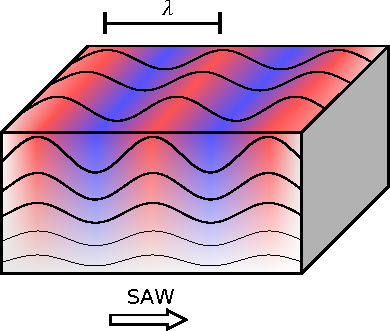
\includegraphics[width = 0.5\textwidth]{SAW intro fig.pdf}
    \caption{A schematic of a surface acoustic wave (SAW) propagating in a piezoelectric substrate. As the SAW mechanically stretches and compresses the piezoelectric, it generates regions of alternating polarization, creating a travelling periodic potential.}
    \label{SAW intro fig}
\end{figure}

This co-propagating SAW electric field interacts with quantum materials, allowing us to probe and control quantum phenomena which are not accessible using conventional transport techniques. Furthermore, the SAW potential extends beyond the surface of the substrate, making it particularly suitable for interfacing with low-dimensional systems.


\section{Many quantum materials are low-dimensional}

This dissertation primarily focuses on low-dimensional materials, or materials which have at least one dimension at the nanoscale, such that electrons are confined to two, one, or zero dimensions. The family of low-dimensional materials includes carbon nanotubes (CNTs) and graphene, which are the primary focus of my work. Spatial confinement, strong Coulomb interactions, and band topology make many low-dimensional materials promising platforms for discovering exotic quantum phenomena with exciting potential applications.

One prominent example of an exotic quantum phenomenon with practical applications is the integer quantum Hall effect. In two-dimensional electron systems under the influence of strong magnetic fields, the Hall conductivity takes quantized integer values \cite{wakabayashi_hall_1978}. Magnetic fields and quantized Landau levels give the quantum Hall system a non-trivial topology, making the Hall conductivity a \textit{topological quantum number} \cite{thouless_quantized_1982}. This understanding of the integer quantum Hall effect as a topological phenomenon ignited interest in the topology of quantum systems, and would later win Thouless et al. the 2016 Nobel Prize in Physics \cite{noauthor_nobel_nodate}. However, study of the quantum Hall effect not only led to new understanding of quantum mechanics, but also practical applications — quantum Hall resistance standards are widely used today to provide a precise measurement of the ohm to parts per billion levels of accuracy. 

Twisted bilayer graphene is another example of a low-dimensional material which exhibits exotic quantum phenomena. By tuning experimental knobs like twist angle, temperature, strain, magnetic field, and carrier concentration, twisted bilayer graphene can be made to exhibit unconventional superconductivity, interaction-induced insulating states, magnetic states, anomalous Hall states, and many more exotic quantum phenomena \cite{andrei_graphene_2020}. These highly tunable exotic quantum phenomena in bilayer graphene exemplify a great strength of low-dimensional materials — because electrons are confined to the surface of low-dimensional materials, we can readily tune their electronic and optical properties.

An example of a tunable electronic property is the valley degree of freedom, which is present in many low-dimensional materials, such as graphene and carbon nanotubes. Within the band structure of a material, a local minimum in the conduction band or a local maximum in the valence band is referred to as a “valley”. Manipulating the shape of an electronic valley has been explored previously in conventional semiconductors, where the shape of a valley is tuned to increase carrier mobility \cite{thompson_90-nm_2004}. However, the usefulness of valleys goes further than just increasing carrier mobility. Graphene has pairs of inequivalent (but degenerate) valleys near the edges of its brillouin zone, at the $K$ and $K'$ symmetry points (Fig.\ \ref{CNT intro fig} (a)). Electrons in the $K$ valley can be labelled as "pseudospin up", and electrons in the $K'$ valley can be labelled as "pseudospin down". These pseudospins have possible applications in "valleytronic" devices which use the pseudospin to store information \cite{schaibley_valleytronics_2016}. 

The reduced dimensionality of low-dimensional materials leads to valley-dependent quantum phenomena which are fundamentally different than in bulk materials. One example is the valley Hall effect in graphene, where electrons in the $K$ and $K'$ valleys were observed to drift in opposite directions under an applied electric field, arising from the topology of graphene's band structure \cite{gorbachev_detecting_2014}. To observe the equal and opposite topological currents of $K$ and $K'$ electrons, it was necessary to use ultraclean encapsulated graphene with low electrostatic disorder, which minimizes disorder-induced inter-valley scattering. In addition to 2D materials, 1D materials such as carbon nanotubes also exhibit interesting valley-dependent physics. 

Carbon nanotubes are essentially rolled-up sheets of graphene, and also possess a valley degree of freedom. During my PhD work, I contributed to a study not included in this dissertation. We grew suspended carbon nanotubes which were measured at low temperature by our collaborators at University of Utah. These ultraclean suspended nanotubes are free of substrate-induced electrostatic disorder, allowing us to observe sensitive quantum phenomena which are not accessible in surface-bound carbon nanotubes. In this study, we demonstrated gate-voltage controlled $K$-$K'$ hybridization of bound electron orbitals (Fig.\ \ref{CNT intro fig} (b)), which could enable future valleytronics devices based on CNTs \cite{berg_vernier_2024}. 

To observe novel phenomena in quantum materials, ultraclean devices like suspended CNTs or encapsulated graphene are a necessity. Much like the need for a clear night sky in astronomy, electrostatic disorder introduces a level of "cloudiness" that obscures our ability to view quantum phenomena. When we minimize electrostatic disorder, it’s as if the clouds part, allowing us to resolve the subtleties of these quantum materials. 

So far, I've discussed quantum phenomena which are accessible with traditional transport techniques, where DC voltage and current is used as a signal. However, surface acoustic waves allow us to probe and control quantum phenomena which are not accessible with traditional transport techniques. 

\begin{figure}
    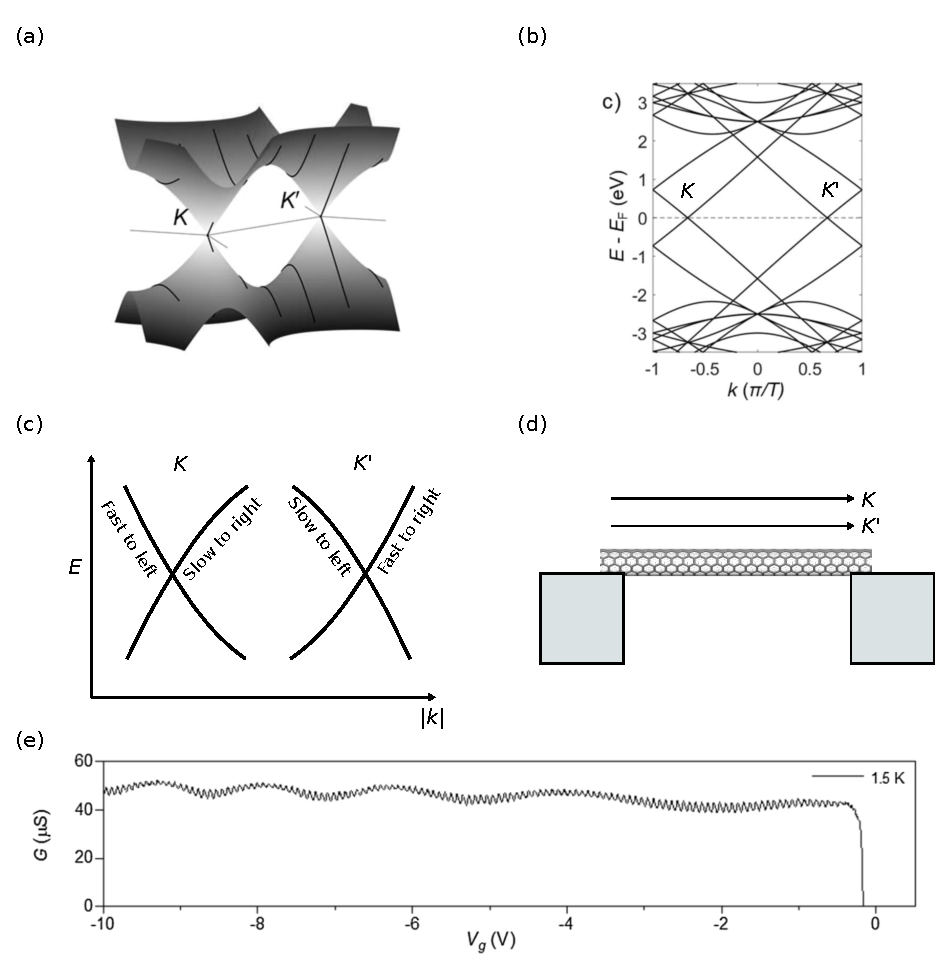
\includegraphics[width = 0.5\textwidth]{CNT intro fig}
    \caption{(a) Zoomed-in band structure of graphene near a pair of $K$ and $K'$ points  (b) In Ref.\ \cite{berg_vernier_2024}, we demonstrate that bound electron states in a suspended CNT can exist in a hybrid state of $K$ and $K'$ orbitals. (Panel (a) was created by Mitchell Senger \cite{senger_optoelectronics_2021}. Reproduced with permission.)}
    \label{CNT intro fig}
\end{figure}

\section{Using surface acoustic waves to probe and control quantum phenomena in 2D systems} \label{using surface acoustic waves to probe and control quantum phenomena}

In this section, I outline three recent works in which surface acoustic waves (SAWs) are used to probe and control quantum phenomena in two-dimensional (2D) systems. These recent works are inspired by a plethora of earlier studies (in the 1980s and 1990s) which utilized SAWs to probe quantum phenomena in GaAs/AlGaAs quantum wells. These earlier SAW-based studies provided new insight into the quantum Hall and fractional quantum Hall effect \cite{wixforth_quantum_1986,esslinger_acoustoelectric_1992,esslinger_ultrasonic_1994,kukushkin_collective_2011,willett_experimental_1993} and Wigner crystallization \cite{paalanen_rf_1992} in GaAs/AlGaAs quantum wells. Building on these successes, researchers have continued to utilize SAWs to probe quantum phenomena in GaAs/AlGaAs quantum wells, and have just begun to explore the potential of SAWs in the rapidly evolving field of layered 2D materials.

As a first example, SAWs have been used to study ordered electron phases in 2D electron systems (2DES). In one work, the authors demonstrated that current-induced modifications of bubble and stripe phases are a local phenomenon \cite{friess_current_2018}. In contrast to prior transport studies which indirectly probe the voltage drop on the edges of the 2DES, the authors used SAWs to probe the entire sample at once, proving that metal contacts cause local perturbations to bubble and stripe phases. Another work used a combination of SAWs, microwave excitation, and optical detection to study quantum Hall stripes \cite{kukushkin_collective_2011}. By employing SAWs with a wavelength of \SI{60}{\nano\meter}, the authors were able to probe commensurability effects between the SAW superlattice and quantum Hall stripes. These works highlight the incredible strength of SAWs for probing the entire bulk of a low-dimensional system at once, circumventing the drawbacks of metal electrodes and local electrostatic gates. 

As a second example, SAWs can be used to transport charge-neutral interlayer excitons in 2D semiconductor bilayers. Transporting charge-neutral excitons is difficult because they exhibit no net force under a uniform electric field. In a recent work, the authors used SAWs to transport charge-neutral interlayer excitons in bilayer WSe\textsubscript{2} \cite{peng_long-range_2022}. Interlayer excitons consist of an electron and hole confined in different real space-separated 2D layers and momentum-space separated valleys \cite{rivera_interlayer_2018}. These excitons are long-lived, allowing them to be transported over long distances, and have large exciton binding energy (due to strong Coulomb interactions between electrons in 2D materials), allowing them to be operational at room temperature. These properties make interlayer excitons promising for nanophotonics and quantum information applications \cite{kuznetsova_all-optical_2010, tran_evidence_2019, liu_electrically_2020}. Prior works utilized diffusion or static gates to transport interlayer excitons, but the transport lengths achievable using these methods are limited \cite{jauregui_electrical_2019,unuchek_room-temperature_2018, liu_electrically_2020}. By leveraging the properties of co-propagating SAW electric fields, the authors of Ref.\ \cite{peng_long-range_2022} demonstrated that interlayer excitons can be transported over distances of $> \SI{30}{\micro\meter}$, an order of magnitude longer than the diffusion length. 

Figure \ref{IX transport fig} illustrates the experiment performed in Ref.\ \cite{peng_long-range_2022}. A SAW traveling in a piezoelectric substrate is accompanied by a co-propagating electric field of the form

\begin{equation}
    E(x, t) = E_0 \mathrm{e}^{i(kx - \omega t)}. 
\end{equation}
As the SAW propagates through the bilayer WSe\textsubscript{2}, this electric field modulates the energy of the interlayer exciton by $U(x,t) = \vectorbold{p} \dotproduct E(x,t)$, where $\vectorbold{p}$ is the dipole moment of the interlayer exciton. This creates potential wells in which charge-neutral excitons can become trapped, "surfing" the SAW potential at the acoustic velocity.

\begin{figure}
    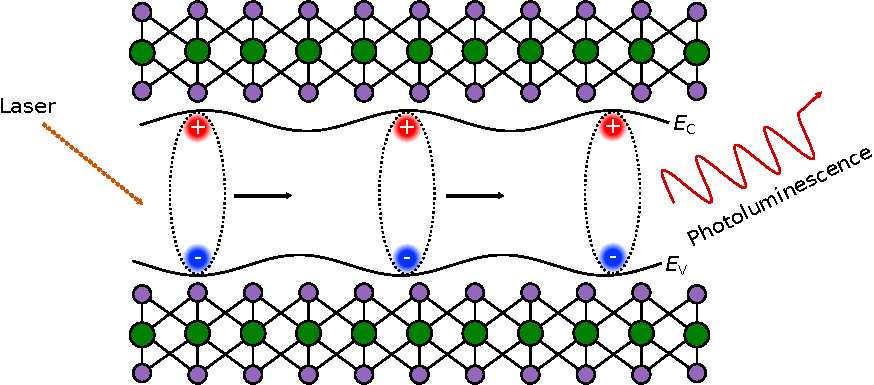
\includegraphics{IX transport fig.pdf}
    \caption{Schematic of the experiment performed in Ref.\ \cite{peng_long-range_2022}. Interlayer excitons consist of bound electrons (blue) and holes (red) confined to the top and bottom layers of bilayer WSe\textsubscript{2}. Excitons generated by laser excitation "surf" the periodic SAW potential up to $\SI{30}{\micro\meter}$ before recombining to create light. The colored circles indicate W (green) and Se (purple) atoms.}
    \label{IX transport fig}
\end{figure}

As a third example, SAWs were recently used as a contactless probe of measuring wave-vector dependent conductivity in ultraclean graphene \cite{fang_quantum_2023}. When SAWs interact with charge carriers in 2D materials, the SAW is attenuated and its velocity is shifted (I discuss SAW attenuation and velocity shift in Sec.\ \ref{SAW theory, propagating in 2D materials}). The authors of Ref.\ \cite{fang_quantum_2023} used this phenomenon to probe quantum Hall transport in ultraclean graphene, solidifying the viability of SAWs as a contactless probe for quantum transport phenomena in 2D materials. 

These three examples have only scratched the surface of what is possible by interfacing SAWs with 2D materials. Many other SAW-induced phenomena in 2D materials have been theoretically predicted, but not yet achieved experimentally (see discussion in Sec.\ \ref{outlook and future work}) \cite{nie_surface_2023}. Further theoretical predictions exist for SAW-enabled phenomena in 1D materials, such as topologically-protected quantized charge transport.

\section{Motivation for future experiments: the Thouless pump} \label{Thouless pump intro chapter}

While many novel surface acoustic wave-driven quantum phenomena have been predicted but not yet realized experimentally (see discussion in Sec.\ \ref{outlook and future work}), topological charge pumping (the "Thouless pump") was a major motivation for the work presented in this dissertation. Though I did not create a Thouless pump, the methods presented in this dissertation represent major steps toward the goal of creating a Thouless pump by coupling a carbon nanotube (CNT) to a surface acoustic wave (SAW).

A charge Thouless pump created by coupling a CNT and SAW would be of great interest to the fields of metrology, where higher-accuracy quantum pumps could help define a better standard of current \cite{pekola_single-electron_2013,scherer_singleelectron_2019}, and quantum computing \cite{das_controlled_2006}, where charge pumps could generate and control the flow of spin-entangled quantum states with minimal decoherence. Though a Thouless pump has been realized in ultracold atoms \cite{citro_thouless_2023}, a charge Thouless pump suitable to serve as a source of quantized current or transport spin-entangled electrons has not yet been created. 

In this section, I overview the Thouless pump system, describing the origin of topologically-protected charge pumping under a periodic potential. Then, I outline practical proposals for a Thouless pump created from a carbon nanotube and SAW, and describe how a Thouless pump could be created from an encapsulated nanotube (with a similar device design to that described in Ch.\ \ref{AE charge pumping paper}), or suspended nanotube (using the flip-chip platform described in Ch.\ \ref{flip-chip chapter}).

\subsection{The Thouless pump: A theoretical perspective}

Topological systems are defined by global properties which are invariant under local perturbations. For example, on a 2D closed surface with local Gaussian curvature $K$, the integral of the Gaussian curvature defines a \textit{topological invariant} called the Euler characteristic ($\chi$). The Gauss-Bonnet theorem defines $\chi$ as

\begin{equation}
    \chi = \frac{1}{2\pi}\iint_S K dA,
\end{equation}
where $S$ is a closed surface. $\chi$ takes only integer values, and is a topological invariant because it is insensitive to deformations of the surface $S$. Figure \ref{surfaces} shows surfaces that all have $\chi = 2$.

\begin{figure}
    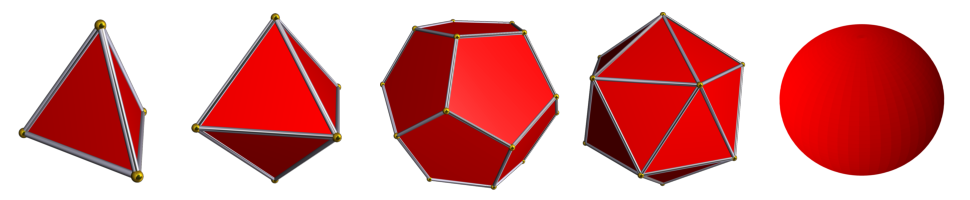
\includegraphics{shapes intro fig.pdf}
    \caption{All of these shapes have an Euler characteristic of $\chi = 2$. A tetrahedron can be smoothly deformed into a sphere, under which transformation $\chi$ is invariant. Images of polyhedra are reproduced from Ref.\ \cite{webb_stella_nodate} under a Creative Commons license.}
    \label{surfaces}
\end{figure}

Similarly, many quantum materials exhibit topological phases of matter, or phases defined by global properties which are insensitive to local perturbations. These global topological properties give rise to \textit{topological quantum numbers} that correspond to physical observables. In a Thouless pump, the system's Hamiltonian undergoes an adiabatic evolution under a spatially- and temporally periodic potential. Thouless found that, though the system begins and ends in the same state (a consequence of the adiabatic theorem — see further discussion in Appx.\ \ref{appendix on topology}), an integer quantity of charge is transported. Thouless concluded that this integer quantity of charge corresponds to a topological invariant called the Chern number, which arises from the topology of the system's band structure.\footnote{More accurately, Thouless's prediction was about \textit{particle transport} in general. In a topological charge pump, the particle being transported is an electron.}

The Thouless pump potential is periodic in space and time. Figure \ref{thouless pump torus} (a) illustrates a potential which is periodic in space, with wavelength $\lambda$, and time, with period $T$. If we take the time axis and the space axis and roll them up, connecting $t = 0$ with $t = T$, and $x = 0$ with $x = \lambda$, one might reason that this spatially- and temporally periodic potential has the topology of a torus. However, the origin of the Chern number in the Thouless pump, and its relation to charge transport, is a bit more subtle. To determine the charge transported during a single cycle of the periodic potential, we need to analyze how a spatially-periodic potential gives rise to quantized energy levels.

The energy eigenstates of electrons in a periodic potential can be described by Bloch wavefunctions, which take the form

\begin{equation}
    \Psi_{nk}(r) = \mathrm{e}^{ikr}u(r), \label{Bloch's theorem}
\end{equation}
where $r$ is the spatial coordinate, $k$ is the momentum vector, $u(r)$ is a function with the same periodicity as the periodic potential ($u(r+ \lambda) = u(r)$), and $n$ is the band index. The wavefunction $\Psi_{nk}(r)$ has associated energy $E_n(k)$. For each value of $k$, an electron can take many valid energies $E_n$. Just like the spatially periodic crystalline structure of materials like silicon or graphene gives rise to band structure, the spatially periodic potential of the Thouless pump also creates energy bands.

Figure \ref{thouless pump torus} (b) illustrates the path of an electron's wavefunction during one cycle of the Thouless pump. The electron wavefunction traverses a closed path in a 2D space spanned by time $t$ and momentum $k$, encircling a filled energy band $E_n$.\footnote{During one cycle of the Thouless pump, the Fermi energy of the system must encircle only filled bands. If the Fermi energy lies above an unfilled band, it allows non-quantized transport of free electrons.} A system which is periodic in two dimensions has the topology of a torus.

\begin{figure}
    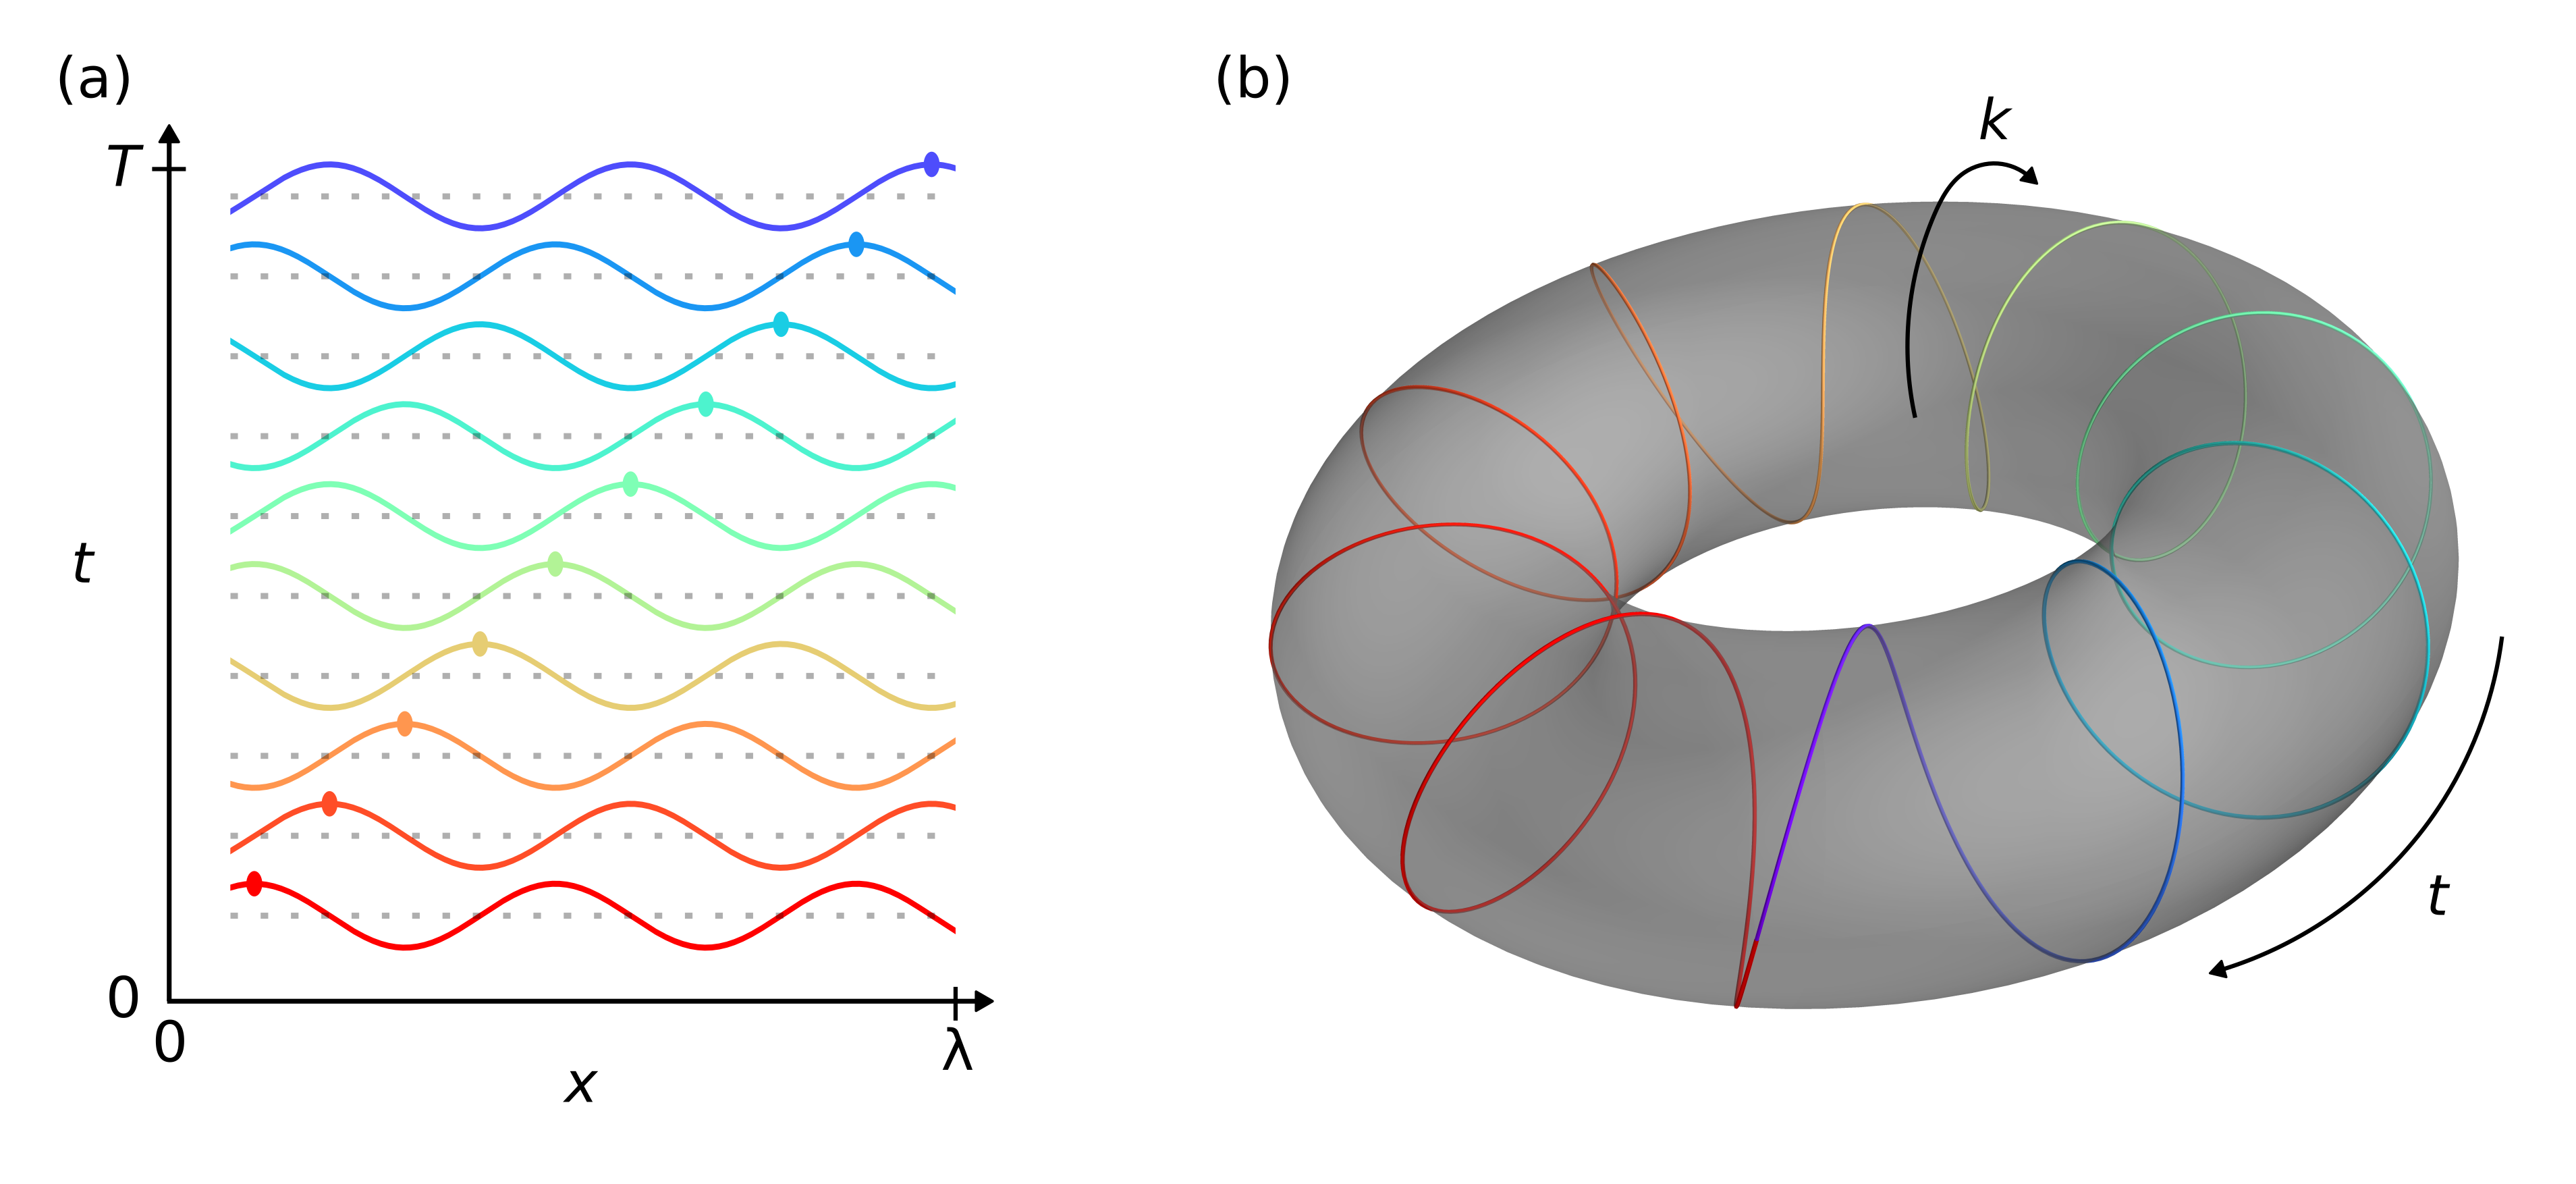
\includegraphics{Thouless pump fig.png}
    \caption{(a) Thouless pumping arises in a system under the influence of a potential which is periodic in real space, $x$, and time, $t$. (b) From Bloch's theorem, periodicity in real space $x$ leads to periodicity in momentum space $k$. The electron wavefunction in a Thouless pump traverses a closed path on a torus in $t\textrm{-}k$ space, encircling an eigenstate of the Hamiltonian \cite{thouless_quantization_1983}.}
    \label{thouless pump torus}
\end{figure}

The last piece of the puzzle to relate charge transport to the Chern number is probability current. In quantum mechanics, wave-particle duality leads to probabilistic predictions about quantum particles. For example, using a particle's wavefunction $\Psi$, we can calculate the probability of finding the particle in-between points a and b to be 

\begin{equation}
    P_{a<x<b} = \int_{a}^{b} |\Psi|^2dx,
\end{equation}
where $|\Psi|^2$ is the probability density of $\Psi$. 

The time evolution of a quantum system satisfies the time-dependent Schrödinger equation,

\begin{equation}
    i \hbar \derivative{t}\ket{\Psi_n} = H(t)\ket{\Psi_n}.
\end{equation}
This wave equation asserts a continuity equation, analogous to continuity equations in fluid dynamics or electromagnetism, which takes the form \cite{sakurai_modern_1985}

\begin{equation}
    \pdv{|\Psi|^2}{t} -\nabla \dotproduct \vectorbold{j} = 0, \label{continuity eqn for probability}
\end{equation}
where $j$ is the \textit{probability flux} or \textit{probability current}, which is given by

\begin{equation}
    j = -\frac{i \hbar}{2 m}\left(\Psi^* \nabla \Psi - (\nabla \Psi^*)\Psi\right). 
\end{equation}
The consequences of this continuity equation can be understood similarly to that in electromagnetism or fluid dynamics. Equation \ref{continuity eqn for probability} states that the amount of probability in a volume can only change if there is a probability flux through the boundary of that volume. Thus, probability is a locally conserved quantity, just like charge or mass. Equation \ref{continuity eqn for probability} also tells us about the flow of the particle described by $\Psi$. If the integral of $j$ at a point in space over a period of time $T$ is equal to one, the probability that a particle passed through that point during that time period 100\%. Thouless related this probability current to the topology of the Thouless pump.

Thouless investigated the probability current $j(k,t)$ integrated over one temporal period $T$ and over all states in a filled band (equivalently, over all momenta in the first Brillouin zone). He found that this integral, which represents a closed path on a torus in $t \textrm{-} k$ space, is equal to the Chern number, which must be an integer \cite{thouless_quantization_1983}. In summary, Thouless found that the Chern number takes the form

\begin{equation}
    C = \frac{1}{2\pi} \int_{0}^{T} \int_{0}^{\frac{2\pi}{\lambda}} j(k,t) dkdt. \label{Thouless Chern equation}
\end{equation}

In the same way that the Gauss-Bonnet theorem links local curvature $K$ of a closed surface to a global topological invariant $\chi$, Thouless found that, when the local probability current $j$ adiabatically traverses a two-dimensional closed path in $t\textrm{-}k$ space, the number of electrons transported over every cycle is exactly the topologically invariant integer Chern number $C$. This topological protection of charge transport, which is predicted to be invariant under perturbations such as local defects or electrostatic disorder, would make a practical charge Thouless pump a powerful experimental tool (see discussion in the next section).

\subsection{Experimental path to a Thouless pump using a carbon nanotube and surface acoustic wave} 

There are numerous experimental challenges for creating a system which behaves like a Thouless pump, and many experimental schemes for Thouless pumping have been proposed \cite{citro_thouless_2023}. However, Talyanskii et al. argue that a CNT coupled to a SAW is the ideal system to create a charge Thouless pump \cite{talyanskii_quantized_2001}. Furthermore, a CNT-SAW Thouless pump could also exhibit novel physics. Theoretical predictions show that the system could pump an average fractional unit of charge per cycle due to the strong electron-electron interactions present in CNTs \cite{novikov_devils_2005}. In this section, I describe how the methods presented in this dissertation could be used to couple a CNT to a SAW to create a Thouless pump. I also discuss the practicality of a CNT-SAW Thouless pump as a source of accurate quantized current.

Charge pumping in CNTs using SAWs has been demonstrated previously \cite{buitelaar_adiabatic_2008}; however, the Thouless pumping regime has not yet been achieved. One reason for this is that it is challenging to fit many spatial periods of the SAW inside an ultraclean CNT. Very long ultraclean CNTs would need to be grown and strongly coupled to SAWs with a very short wavelength. Also, insulating surfaces, including piezoelectric insulators (on which SAWs are generated), induce considerable electrostatic disorder within electronic systems on their surface. Therefore, surface-bound CNTs (such as in Ref.\ \cite{buitelaar_adiabatic_2008}) are too disordered to use in a Thouless pump. Thus, to create a charge Thouless pump from a CNT, we must turn to demonstrated methods of creating ultraclean CNTs: Either encapsulate the CNT in two-dimensional hexagonal boron nitride (h-BN) \cite{huang_superior_2015}, or suspend the CNT above the substrate \cite{senger_universal_2018}. Figure \ref{Thouless pump designs} illustrates possible device designs for these two scenarios.


\begin{figure}
    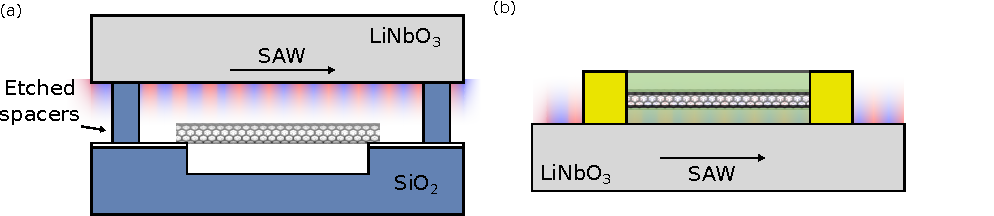
\includegraphics{Intro thouless pump designs.pdf}
    \caption{Two possible device designs for interfacing ultraclean CNTs with SAWs. (a) A suspended CNT and SAW device could be fabricated on two separate chips and interfaced using flip-chip construction. (b) Surface-bound CNTs could be grown on a separate substrate, encapsulated in h-BN (as in Ref.\ \cite{huang_superior_2015}), and transferred next to a SAW device.}
    \label{Thouless pump designs}
\end{figure}

On its face, marrying a surface acoustic wave and suspended CNT to create a charge Thouless pump does not seem too challenging. It is possible to create \SI{3}{\micro\meter}-long ultraclean suspended CNTs \cite{senger_universal_2018}, and SAWs with \SI{60}{\nano\meter} wavelength have been coupled to quantum materials before \cite{kukushkin_collective_2011}. Such a system would have 50 spatial periods of the SAW inside the CNT. However, growing CNTs and generating SAWs have competing fabrication requirements. To couple a SAW to a suspended CNT, we would need to fabricate the two chips separately, and bring them into extremely close contact to . A technique called "flip-chip construction" has emerged in recent years, in which a gate chip is "flipped" onto a quantum material to non-invasively gate the material. In Ch.\ \ref{flip-chip chapter}, I present a method of flip-chip construction that allows the air gap between the two chips to be precisely measured. Figure \ref{Thouless pump designs} (a) illustrates how my flip-chip design could be used to couple SAWs to a suspended CNT.

Another possibility would be to encapsulate a CNT in hexagonal boron nitride (h-BN) and transfer it to a piezoelectric substrate (Fig. \ref{Thouless pump designs} (b)). In Ref.\ \cite{huang_superior_2015}, the authors encapsulate a CNT in h-BN using a similar dry transfer technique to the one that I outline in Sec.\ \ref{transfer methods section}. In Ch.\ \ref{AE charge pumping paper}, I encapsulate graphene in h-BN and transfer it onto LiNbO\textsubscript{3}, then generate SAWs to pump charge through the graphene. To create a charge Thouless pump, a CNT could similarly be encapsulated in h-BN and transferred onto a LiNbO\textsubscript{3} substrate next to a SAW device. Then, one-dimensional contacts (as in Ref.\ \cite{huang_superior_2015}) could be made to the CNT. One concern for this approach is residues contaminating the CNT during the transfer process. To clean the encapsulated CNT, contact mode atomic force microscopy could be used to "squeegee" out any contaminants stuck between the h-BN layers, similarly to the process I describe in Sec.\ \ref{AFM cleaning main section} \cite{goossens_mechanical_2012,chen_tip-based_2021}. 

One might wonder: Can a real-world Thouless pump ever generate accurate quantized current? A critical requirement of the Thouless pump is the adiabatic approximation, which asserts that the state of the system must remain in a gap of the Hamiltonian during the entirety of its cyclic evolution. Furthermore, Thouless studied an infinite 1D system, which is clearly nonphysical. However, prior authors argued that a real Thouless pump could provide accurate quantized current, despite perturbations from the environment \cite{niu_towards_1990, niu_quantised_1984}. These authors considered perturbations which could cause electrons in a periodic potential to close the energy gap $\Delta$, such as thermally excited carriers, nonadiabatic excitations, tunneling from one side of the 1D wire to the other, and electrostatic disorder. All of these perturbations could break the adiabatic approximation, causing charge transport that does not adhere to an integer quantity of charge per cycle. Ref.\ \cite{niu_towards_1990} considered an energy gap of $\Delta \approx \SI{1}{\milli\electronvolt}$ and found the error in quantized charge transpsort from these environmental perturbations to be exponentially small, concluding that a real-world Thouless pump could provide parts-per-billion levels of accuracy if the 1D system is many times longer than the spatial period of the periodic potential. The later theoretical study of a CNT-SAW Thouless pump by Talyanskii et al. estimated the gaps in the system's band structure to be $\Delta \approx \SI{10}{\milli\electronvolt}$ \cite{talyanskii_quantized_2001}. Therefore, errors to the accuracy of a CNT-SAW Thouless pump can be controlled to provide quantized current with parts-per-billion accuracy. 

Many designs for quantized charge pumps have been demonstrated, with the best sources of quantized current today being based on controlling tunneling to- and from quantum dots \cite{scherer_singleelectron_2019}. However, charge pumps based on tunneling face fundamental limits to their accuracy. From the above considerations, a topologically-protected charge pump created from a CNT and SAW could provide accurate quantized current beyond what is possible with tunneling-based charge pumps.

%From this, and using the order-of-magnitude estimates of the errors due to environmental perturbation given by Ref.\ \cite{niu_towards_1990}, I can estimate the accuracy of a CNT-SAW Thouless pump system. The error due to thermally-excited carriers is $\exp(-\Delta/kT) \approx 1\times 10^{-13}$ (at T = \SI{4}{\kelvin}, easily achievable in modern cryostats), the error due to nonadiabatic excitations is $\exp(-\Delta/h f) \approx 1\times 10^{-53}$ (at a very high SAW frequency of $f = \SI{20}{\giga\hertz}$), and 


\section{Outline}
In this dissertation, I discuss my work in developing methods for interfacing 2D and 1D materials with surface acoustic waves (SAWs). In Chapter \ref{methods chapter}, I outline the tricks that I have learned for creating 2D devices. I first present my process for exfoliating 2D flakes. Then, I describe in detail the hot pickup technique for stacking 2D materials to create heterostructures. I continue by describing a method of using a highly-adhesive polymer to remove unwanted 2D flakes from a substrate, which is a crucial part of fabricating the devices described in Ch.\ \ref{AE charge pumping paper}, as SAW devices can easily be short-circuited by transfer of unwanted graphene flakes. I also describe a method of cleaning metal contacts with contact-mode AFM before transferring 2D flakes onto them. Finally, I outline design rules for fabricating SAW devices and methods for measuring their frequency response. 

In Ch.\ \ref{AE charge pumping paper}, I show measurements of acoustoelectric charge pumping in h-BN-encapsulated graphene that I performed. These are the first measurements of charge pumping in encapsulated graphene presented in literature. I then describe a model for mixed-carrier acoustoelectric transport in graphene. Our model extends the single-carrier classical relaxation model described in Sec.\ \ref{classical relaxtion model} to account for coexistence of electrons and holes in graphene near the charge neutrality point. I fit this mixed-carrier model to two acoustoelectric graphene devices with different levels of electrostatic disorder, and demonstrate excellent agreement between the model and experimental data.

In Ch.\ \ref{flip-chip chapter}, I describe my design for interfacing pristine quantum materials with surface acoustic waves using flip-chip construction. I improve on prior flip-chip designs by precisely measuring the air gap between the top and bottom chips using both a novel reflectance spectroscopy method and capacitance method. I demonstrate that I can achieve a small air gap of $\approx \SI{0.7}{\micro\meter}$, and discuss the possibilities of this design for future SAW-based probes of quantum materials.


\chapter{Theory}

In this chapter, I first present the linear band structure of graphene and use it to derive an expression for the density of states near the Dirac points. Using the density of states, I calculate the thermally excited electron and hole densities in ultraclean, undoped graphene. We use this calculation in Ch.\ \ref{AE charge pumping paper} to compare the carrier density in our graphene samples with the lowest achievable carrier density at room temperature.

\section{The electronic properties of graphene} \label{the electronic properties of graphene}

Graphene consists of a single layer of carbon atoms in a hexagonal lattice. The band structure of graphene is well-described by a tight binding model, where only hopping energy between nearest neighbor atoms is considered \cite{wallace_band_1947}. From the tight binding model, the dispersion relation of graphene is 

\begin{equation}
    E(k_x, k_y) = \pm t  \left(3 + 2\mathrm{cos}(\sqrt{3}k_x a) + 4\mathrm{cos}(\frac{3}{2}k_y a)\mathrm{cos}(\frac{\sqrt{3}}{2}k_x a)\right)^{1/2}, \label{graphene dispersion}
\end{equation}
where $k = (k_x, k_y)$ is the momentum vector of electrons in the graphene, $t = 2.8 \; eV$ is the nearest-neighbor hopping energy, and $a = 1.42 \;\SIUnitSymbolAngstrom$ is the distance between the two nearest neighbor atoms. Figure \ref{graphene dispersion plot} (a) shows a plot of the band structure given by Eq.\ \ref{graphene dispersion}.


\begin{figure}
    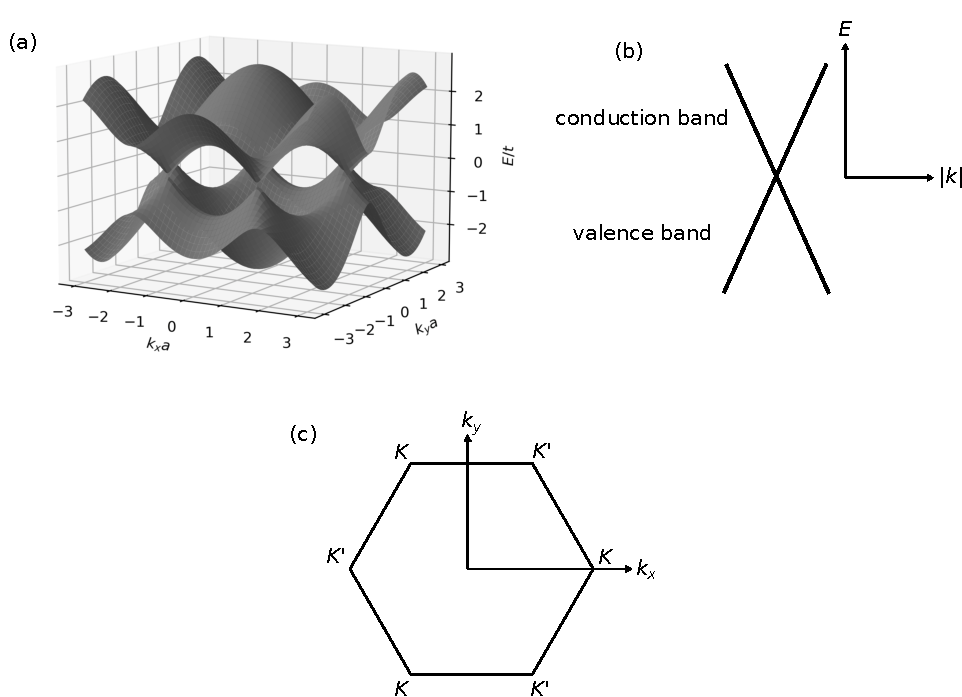
\includegraphics[width = 1\textwidth]{Graphene band structure 3D.pdf}
    \caption{(a) A plot of graphene's dispersion relation given by Eq.\ \ref{graphene dispersion}. (b) Near a Dirac point, the energy of electronic states in graphene is approximately linear with respect to momentum. (c) The momentum-space lattice of graphene, with Dirac points labelled.}
    \label{graphene dispersion plot}
\end{figure}
In charge-neutral graphene, the Fermi energy $E_F$ (the energy of the highest filled state at zero temperature) intersects the bands at symmetry points called the $K$ and $K'$ points, also known as the Dirac points (Figure \ref{graphene dispersion plot} (c)). Near the Dirac points, graphene's dispersion relation is linear, and can be approximated as

%TODO: Look through uses of "approx" and make sure there is appropriate space between the approx symbol and the number after it 

\begin{equation}
    E(k) \approx \pm \hbar v_f \abs{k}, \label{linear dispersion of graphene}
\end{equation}
where $k$ is the distance from the $K$ and $K'$ points, $\hbar$ is the reduced Planck's constant, and $v_f = 3ta/2 \approx \SI{e6}{\meter/\second}$ is the Fermi velocity. Figure \ref{graphene dispersion plot} (b) offers a magnified view of graphene's band structure near a Dirac point, showing its characteristic shape commonly referred to as the "Dirac cone". In conventional semiconductors and metals, we expect a parabolic energy-momentum relation of $E(k) = k^2/2m$, which gives a velocity of $v = \sqrt{2E/m}$. However, in the case of graphene, electrons near a Dirac point move at a velocity $v_F$ which is independent of both energy and momentum, leading to many unique electronic properties \cite{castro_neto_electronic_2009}. For example, electrons and holes in graphene behave almost identically, in contrast to other materials \cite{novoselov_electronic_2007,castro_neto_electronic_2009}. In the context of this dissertation, electron-hole symmetry is the most pertinent consequence of graphene’s unique band structure.

In graphene, we can tune the Fermi energy using an electric field, which in turn tunes the charge carrier density.\footnote{The term "charge carrier" or "carrier" is commonly used to refer to both electrons and holes, and I use it in this context throughout this dissertation.} Figure \ref{graphene bands at 0 T} illustrates graphene's band structure at zero temperature for $E_F < 0$, $E_F = 0$, and $E_F < 0$. When $E_F$ lies above the Dirac point ($E_F > 0$), states in the conduction band are filled with electrons up to $E_F$ (Fig.\ \ref{graphene bands at 0 T} (a)). Conversely, when $E_F < 0$, the valence band is depleted of electrons down to $E_F$ (Fig.\ \ref{graphene bands at 0 T} (c)). These vacant electronic states, referred to as "holes", act as positively-charged quasiparticles. Similar to electrons in the conduction band, holes in the valence band are free from the graphene lattice and can move in response to an electric field. In the case of charge neutral graphene ($E_F$ = 0) at zero temperature, the conduction band is entirely empty, and the valence band is completely occupied, so no charge carriers should be present to conduct current (Fig.\ \ref{graphene bands at 0 T} (b)). However, at finite temperature, charge carriers can still be present when $E_F = 0$, leading to finite conductivity when $E_F$ is tuned to the charge neutrality point.
\begin{figure}
    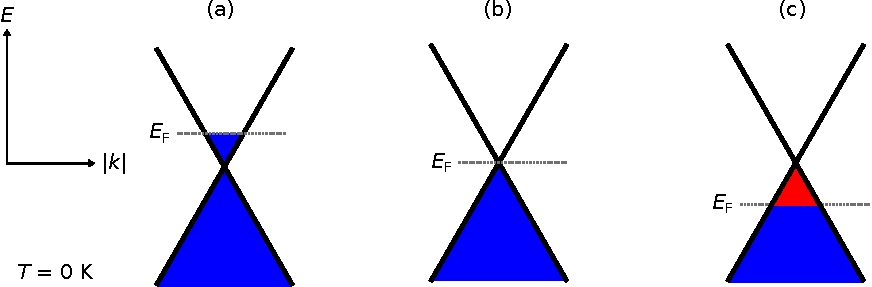
\includegraphics{graphene theory 0}
    \caption{Filling of electronic states in graphene at zero temperature for (a) $E_F >0$, (b) $E_F = 0$, and (c) $E_F < 0$. Filled electronic states are indicated in blue. Unfilled electronic states in the valence band (holes) are indicated in red.}
    \label{graphene bands at 0 T}
\end{figure}

Extrinsic sources of charge, referred to as electrostatic disorder, can be present in real graphene samples. For instance, substrates like SiO\textsubscript{2} contain charge traps which induce spatially-varying charge carrier concentrations in graphene \cite{martin_observation_2008}. This substrate-induced disorder can be minimized by encapsulating graphene in hexagonal boron nitride (h-BN) \cite{dean_boron_2010}. However, even the most pristine encapsulated graphene samples exhibit some DC conductivity at the charge neutrality point \cite{xin_giant_2023} due to thermally-excited electrons and holes. To quantify the densities of these thermally excited electrons and holes, I will proceed to derive the density of states in graphene.

\subsection{Density of states in graphene}
The density of states tells us how many states are available for electrons to occupy at a certain energy level. Consider a sheet of graphene at zero temperature in which we have tuned the Fermi energy $E_F$ to lie above the Dirac point, filling the states in the conduction band with electrons to an energy $E_F$. Figure \ref{density of states graphic} (b) illustrates the $k$-plane slice at $E = E_F$, where the momentum at which $E_F$ intersects the Dirac cone is defined as $k_F$. To find the density of states, we can count the number of states that lie inside this circle (states with momentum $0 < k < k_F$), and divide this number by the area of a single state in momentum space.

\begin{figure}
    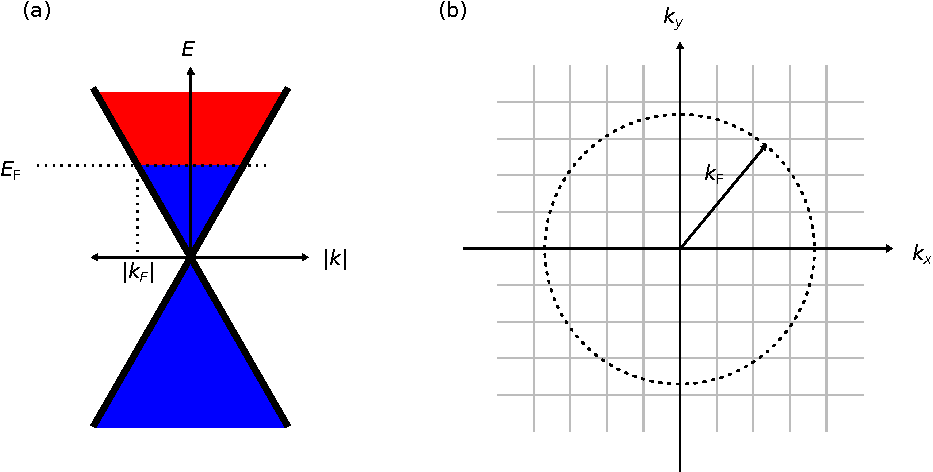
\includegraphics[width = 0.75\textwidth]{density of states graphic.pdf}
    \caption{(a) Graphene band diagram with the Fermi energy indicated by $E_F$. (b) The $k_x$ - $k_y$ plane at $E = E_F$. The intersection of the Dirac cone with this plane forms a circle with radius $|k_F|$.}
    \label{density of states graphic}
\end{figure}
The graphene lattice is periodic, so the spatial part of the electron wavefunction must also be periodic. If the graphene real-space periodicity is $a$ (or, the unit cell has area $a^2$ in real space), then the allowable momenta are integer multiples of $(k_x, k_y) = (2\pi/a, 2\pi/a)$. Thus, a single occupied state takes up an area of $(2\pi/a)^2$ in momentum space. The total number of states with $k < k_F$ is given by the area of our circle of radius $k_F$ divided by the area of a single state,

\begin{equation}
    N = \frac{\pi k_F^2}{(2\pi/a)^2} = \frac{k_F^2 a^2}{4\pi}. 
\end{equation}
Then, the density of states is given by 

\begin{equation}
    D(E_F) = \frac{4}{a^2} \derivative{N}{k_F} = 4\frac{(2k_F)}{4 \pi} = \frac{2\abs{E_F}}{\pi \hbar^2 v_F^2}, \label{graphene DOS}
\end{equation}
where the factor of 4 originates from graphene's four-fold degeneracy of two valleys ($K$ and $K'$) and two spins (spin up and spin down), and the absolute value ensures that $D(E)$ is a positive quantity. Equation \ref{graphene DOS} elucidates why graphene is a semimetal — though graphene has no band gap, the density of states is zero at the Fermi energy in charge-neutral graphene. However, thermal energy can excite charge carriers to occupy states that are not at the Fermi energy.

\subsection{Thermally excited charge carriers in graphene at finite temperature}
At finite temperatures, electrons will be thermally excited into the conduction band, leaving holes in the valence band. These thermally excited electrons and holes can contribute to conduction, and limit the lowest achievable carrier density (and lowest achievable conductance) in charge-neutral graphene at finite temperature. Figure \ref{graphene at elevated T plot} illustrates the thermally-excited electron and hole populations near the Fermi energy. 
\begin{figure}
    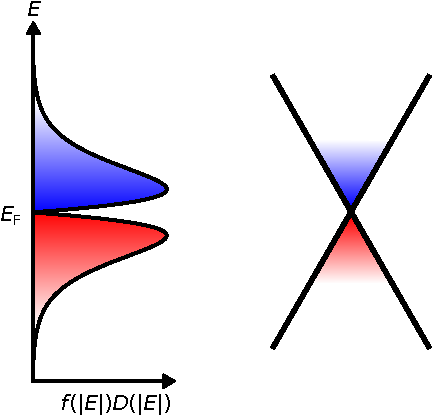
\includegraphics{graphene theory 3.pdf}
    \caption{A plot of $f(|E|)D(|E|)$ with respect to energy $E$ for graphene at elevated temperature (left) next to graphene's dispersion relation (right). The colors represent free electrons (blue) and free holes (red). The color intensity represents the magnitude of $f(E)$ (for electrons) and ($1-f(E)$) (for holes).}
    \label{graphene at elevated T plot}
\end{figure}
The thermally excited electron and hole densities $n$ and $p$ are given by

\begin{gather}
        n = \int_{0}^{\infty}f(E) D(E)\mathrm{d}E, \label{n integral} \\ 
        p = \int_{-\infty}^{0}(1- f(E)) D(E)\mathrm{d}E, \label{p integral}
\end{gather}

where $f(E)$ is the Fermi occupation function, which takes the form

\begin{equation}
    f(E) = \frac{1}{1+\mathrm{e}^{(E-\mu_{\mathrm{chem}})/k_B T}},
\end{equation}
where $\mu_{\mathrm{chem}}$ is the chemical potential, $k_B$ is Boltzmann's constant, and $T$ is temperature. I take $\mu_{\mathrm{chem}} = 0$ to describe charge neutral graphene. 

Equations \ref{n integral} and \ref{p integral} can be solved analytically as follows:

\begin{equation}
    \begin{split}
        n = \int_{0}^{\infty}f(E) D(E)\mathrm{d}E 
        = \int_{0}^{\infty}\frac{1}{1+\mathrm{e}^{(E/k_B T)}} \frac{2E}{\pi \hbar^2 v_F^2}\mathrm{d}E \\
        = \frac{2(k_B T)^2}{\pi \hbar^2 v_F^2}\int_{0}^{\infty}\frac{x}{1+\mathrm{e}^{x}}\mathrm{d}x \\
        = \frac{2(k_B T)^2}{\pi\hbar^2 v_F^2} \frac{\pi^2}{12}, \label{n density}
    \end{split}
\end{equation}
\begin{equation}
    \begin{split}
        p = \int_{-\infty}^{0}(1-f(E)) D(E)\mathrm{d}E 
        = \int_{-\infty}^{0}\left( 1 -\frac{1}{1+\mathrm{e}^{(E/k_B T)}} \right) \frac{-2E}{\pi \hbar^2 v_F^2}\mathrm{d}E \\
        = -\frac{2(k_B T)^2}{\pi \hbar^2 v_F^2}\int_{-\infty}^{0}\left(x - \frac{x}{1+\mathrm{e}^{x}}\right)\mathrm{d}x \\
        = \frac{2(k_B T)^2}{\pi\hbar^2 v_F^2} \frac{\pi^2}{12}, \label{p density}
    \end{split}
\end{equation}
where I use the substitution $x = E/(k_B T)$ to evaluate the integral, and an extra negative sign arises in the right side of Eq.\ \ref{p density} due to $|E|$. Both $n$ and $p$ yield identical expressions, which is consistent with the symmetry of graphene's band structure above and below $E = 0$ near the Dirac point. From Eqs. \ref{n density} and \ref{p density}, I calculate the minimum achievable carrier densities at $T = $ \SI{300}{\kelvin} to be $n = p \approx $\SI{0.08e12}{\centi\meter^{-2}}. Therefore, the total free carrier density in graphene at $T = $ \SI{300}{\kelvin} is $\approx \SI{0.16e12}{\centi\meter^{-2}}$. This result is used in Ch.\ \ref{AE charge pumping paper} to quantify the minimum carrier density achievable in our graphene sample, and is integral to understanding the behavior of our graphene device at the charge neutrality point.

Electrons and holes have equal and opposite charge, and thus move in opposite directions under a DC electric field (for example, when an external voltage bias is applied). Whether graphene is populated by electrons or holes, conventional current will flow in the same direction under an applied DC electric field (the sign of conventional current is the same whether an electron is moving left or a hole is moving right). Therefore, thermally excited electrons and holes cause a nonzero current to flow in a graphene device at the charge neutrality point. However, the same is not true for acoustoelectric current. In an acoustoelectric device, the sign of current reverses between electron transport and hole transport. This results in zero net current at the charge neutrality point, despite a nonzero thermally-excited carrier concentration (as in the graphene charge pumping results in Sec.\ \ref{AE charge pumping results}). In the next section, I derive the expression for acoustoelectric current in a thin film, which predicts that surface acoustic waves push both electrons and holes in the same direction, and forms the basis for the mixed-carrier classical relaxation model presented in Sec.\ \ref{AE paper discussion}.

\section{Surface acoustic waves and acoustoelectric charge pumping}

A surface acoustic wave (SAW) is an elastic wave that propagates along the surface of a material, with its energy confined to a depth of around one wavelength below the surface \cite{rayleigh_waves_1885}. When a SAW propagates in a piezoelectric substrate, it mechanically stresses the piezoelectric, generating electric fields. In turn, these electric fields generate strain in the substrate. If we coat this piezoelectric surface with a thin film, the SAW feels and responds to electronic and mechanical properties of the film (in this dissertation the thin film of interest is graphene). This interplay between a SAW and its propagation environment make SAWs interesting both as a method for probing phenomena in quantum materials (see Sec.\ \ref{using surface acoustic waves to probe and control quantum phenomena}), and for using the interaction between a SAW and quantum material to probe the environment, such as in gas sensors and humidity sensors \cite{yang_gas_2017}. These applications largely use the attenuation and velocity shift of a SAW by a semiconducting thin film (or 2D material, such as graphene) as their sensing signal. Also, in Ch.\ \ref{AE charge pumping paper}, I use SAWs to pump charge through encapsulated graphene. Therefore, I need to develop an understanding of SAW propagation in piezoelectric substrates and the interaction of SAWs with the environment in which they propagate. As we will see, a one-dimensional model of longitudinal SAWs is sufficient to develop this understanding. 

I begin this section with a discussion of elastic waves in bulk non-piezoelectric materials and derive the corresponding wave equation. Then, I discuss waves in bulk piezoelectric materials and explore how the effective stiffness of the piezoelectric substrate varies in cases of very low or very high bulk conductivity. Next, I consider the intermediate conductivity case and derive the bulk conductivity-dependent attenuation and velocity shift equations. Finally, I discuss how the velocity shift and attenuation change when the conductivity is located in a thin film on an insulating piezoelectric surface, and how the attenuation drives a DC acoustoelectric current in the thin film. This sets the stage for the later Sec.\ \ref{AE paper discussion}, where I modify these equations to consider mixed-carrier transport in graphene. The discussion in this section follows that of Refs. \cite{datta_surface_1986, weinreich_acoustodynamic_1956, hutson_elastic_1962, wixforth_surface_1989}, except where noted by additional references.

\subsection{Elastic waves in non-piezoelectric materials}
To understand the propagation of SAWs in piezoelectric materials, we must first understand the constitutive equation of waves in bulk elastic materials. The constitutive equation relates the spatial variations in the displacement of internal elements of this elastic material, known as "strain" (a dimensionless quantity), to the internal forces which caused the strain, known as "stress" (dimensions of force per unit area). The relationship between stress and strain determines how elastic waves propagate. 

Consider a rod with initial length $L$ which is deformed to a length $L + \Delta$ by an applied force $F$ (Fig.\ \ref{dfield}). The displacement $u$ of a particle in the rod from the unstrained condition varies linearly over distance $x$. Strain, denoted by $S$, is defined by the local rate of change of $u$ over distance, 

\begin{equation}
    S = \pdv{u}{x}. \label{strain-displacement equation}
\end{equation}
This is a one-dimensional model, so I do not consider shear strains.

\begin{figure}
    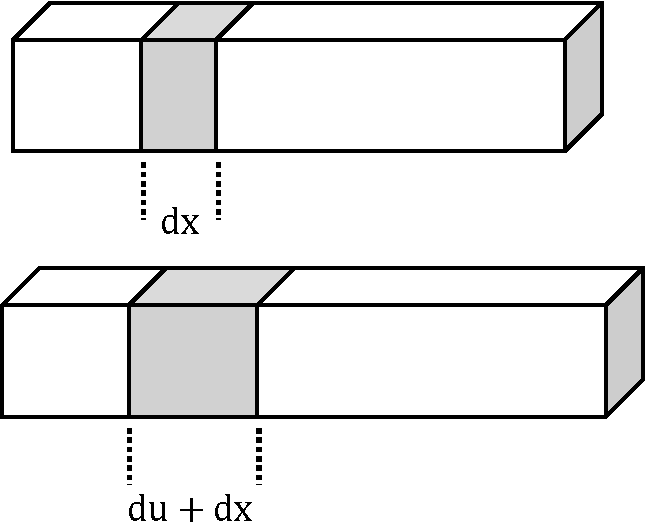
\includegraphics{displacement field.pdf}
    \caption{(a) An illustration of an element which deforms from length $L$ to length $L + \Delta$. (b) The displacement $u$ of a particle in the rod from its unstressed position varies linearly with distance $x$.} \label{dfield}
\end{figure}
Stress, denoted by $T$ (not to be confused with temperature!), is related to strain by the constitutive equation

\begin{equation}
    T = cS, \label{elastic Hooke's}
\end{equation}
where $c$ is the stiffness coefficient, also known as Young's modulus. This is a generalization of Hooke's law, with a linear relationship between strain and stress. Stress $T$ is related to $u$ by 

\begin{equation}
    \pdv{T}{x} = \rho \pdv[2]{u}{t}, \label{stress related to displacement}
\end{equation}
where $\rho$ is the mass density of the material. From these relations, we get an equation for waves in elastic materials

\begin{equation}
    \pdv[2]{u}{t} = \frac{c}{\rho} \pdv[2]{u}{x},
\end{equation}
from which we can readily see that plane waves propagate in this elastic material with a velocity $v_0 = \sqrt{c/\rho}$. This is familiar from traveling acoustic waves in a tensioned string: as tension increases, waves propagate more quickly, and as mass density increases, waves propagate more slowly. In piezoelectric materials, this intuition holds, with one caveat: the effective stiffness of a piezoelectric material depends on more than just its mechanical properties.

\subsection{Elastic waves in bulk piezoelectric materials} \label{waves in bulk piezoelectric materials}
\begin{figure}
    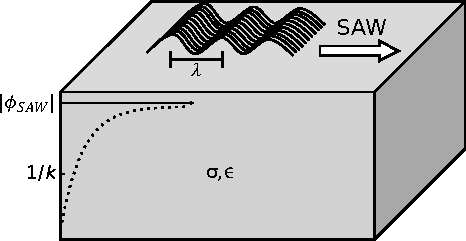
\includegraphics[width = 0.6\textwidth]{SAW in bulk semi.pdf}
    \caption{A surface acoustic wave traveling in a bulk piezoelectric material. The SAW amplitude $|\phi_{SAW}|$ is well-known to decay approximately exponentially into the surface, with most of its energy contained within a depth $1/k$ \cite{wixforth_surface_1989}.}
    \label{SAWbulksemi}
\end{figure}
Consider a surface acoustic wave with wave vector $k$ propagating in a bulk piezoelectric material with conductivity $\sigma$ and dielectric permittivity $\epsilon$, shown in Fig.\ \ref{SAWbulksemi}. In a piezoelectric material, strain creates displacement fields ($D$-fields), and electric fields create stress. This translates to new constitutive equations for waves in piezoelectric materials. Take caution here to not confuse displacement field $D$ with spatial displacement $u$! 

For small $u$, the constitutive equations of waves in a piezoelectric material are

\begin{equation} 
    D = eS + \epsilon E \label{Delastic}
\end{equation}
and
\begin{equation} 
    T = cS -eE, \label{Telastic}
\end{equation}
where $e$ is the piezoelectric constant (assumed here to cause electric fields only in the $x$-direction), $c$ is the elastic constant at constant electric field, and $\epsilon$ is the dielectric permittivity at constant strain. Remembering the definition of displacement field $D = \epsilon E + P$, where $P$ is polarization, we can see from Eq.\ \ref{Delastic} that the strength of polarization in piezoelectric materials scales with the piezoelectric constant $e$, and strain creates a polarization $P = eS$. Equation \ref{Telastic} can be thought of as the same generalized Hooke's law from Eq.\ \ref{elastic Hooke's}, but with additional stress $-eE$ arising from the piezoelectric effect. 

We are interested in the interaction of SAWs with conducting films, and Eqs. \ref{Delastic} and \ref{Telastic} do not include conductivity (denoted here by $\sigma$). To introduce the effect of conductivity on the constitutive equations, I first consider limiting cases of very high $\sigma$ and very low $\sigma$. I simplify the analysis by assuming uniform conductivity through the bulk of the piezoelectric, rather than a thin conducting film. Then, in Sec.\ \ref{SAW theory, propagating in 2D materials}, I discuss how this model can be modified to describe thin conducting films on a piezoelectric insulator.

In a piezoelectric material with $\sigma = \infty$, $E = 0$ because the material can screen all internal electric fields, and the piezoelectric constitutive equations reduce to 

\begin{equation}
    T = cS
\end{equation}
and
\begin{equation}
    D = eS.
\end{equation}
In this case, our wave velocity is $v_0 = \sqrt{c/\rho}$ (unchanged from before), and the elastic wave propagates in tandem with $D$-fields. This case of a material with very high conductivity is framed by Wixforth et al.  as "a material that [to the elastic wave] appears to be non-piezoelectric" \cite{wixforth_surface_1989}.

The next limiting case is that of very low conductivity ($\sigma = 0$). In this perfect piezoelectric insulator, there is no free charge, so Poisson's equation requires that 

\begin{equation}
    \pdv{D}{x} = 0.
\end{equation}
Rearranging Eqs. \ref{Delastic} and \ref{Telastic}, we find that the wave equation for our piezoelectric insulator is

\begin{equation}
    \pdv[2]{u}{t} = \frac{c}{\rho} (1 + \frac{e^2}{2c\epsilon}) \pdv[2]{u}{x}. \label{wave eqn for insulator}
\end{equation}
Defining $c^* = c(1 + e^2/c\epsilon)$, this describes a wave traveling at a velocity $v^* =\sqrt{c^*/\rho}$. The piezoelectric interaction has caused our effective elastic constant to increase by a factor $e^2/2c\epsilon$! This quantity is known as the "piezoelectric coupling constant", denoted $K^2 = e^2/c\epsilon$, which represents the ratio of coupled piezoelectric energy to total stored energy. Total stored energy includes energy stored both in the D-fields (scaling with $\epsilon$) and in mechanical deformation (scaling with $c$). 

$K^2$ varies widely between materials, ranging from $6.4 \times 10^{-4}$ in GaAs \cite{wixforth_surface_1989} to 0.05 in LiNbO\textsubscript{3} \cite{warner_determination_1967}. Stronger piezoelectric interactions (increasing $e$) stiffen the material; conversely, a stronger dielectric (increasing $\epsilon$) softens the material. This effective increase in elastic constant from piezoelectric interactions is known as "piezoelectric stiffening" and has important consequences for interactions between SAWs and charge carriers in thin films, as will be seen shortly. 

Next, we tackle the case of intermediate $\sigma$, i.e., the case of a piezoelectric semiconductor. In this dissertation, acoustic waves in a piezoelectric semiconductor are particularly interesting because the physics is similar whether $\sigma$ is contained in the bulk piezoelectric or in a thin film on an insulating piezoelectric (like graphene on LiNbO\textsubscript{3}). 

The current density $J$ in a semiconductor is the sum of the drift and diffusion currents

\begin{equation}
    J = q n \mu E + \frac{\mu}{\beta} \pdv{n}{x}, \label{jdiff}
\end{equation}
where q is the electron charge, $\beta$ is the inverse of Boltzmann's constant times temperature, and $n$ is the carrier density (assumed here to be populated only by electrons). Here, I assume the limiting case where drift current is much larger than diffusion current, so diffusion can be neglected. Differentiating Eq.\ \ref{jdiff} (neglecting diffusion), we have

\begin{equation}
    \pdv{J}{x} = \mu q \pdv{E}{x}. \label{djdx}
\end{equation}
Using Poisson's equation $\pdv*{D}{x} = -qn$ and the continuity equation $\pdv*{J}{x} = q \pdv*{n}{t}$, Eq.\ \ref{djdx} becomes

\begin{equation}
    \pdv{D}{x}{t} = -\mu q n \pdv{E}{x}. \label{Ddxt}
\end{equation}
Assuming the $E$ and $D$ fields generated by our SAW take the form of plane waves $E = E_0 \mathrm{exp}(i(kx - \omega t))$ and $D = D_0 \mathrm{exp}(i(kx - \omega t))$, Eq.\ \ref{Ddxt} becomes

\begin{equation}
    D = -i\frac{\sigma}{\omega} E, \label{DinE}
\end{equation}
where $\sigma = \mu n q$ is the conductivity of the piezoelectric semiconductor. Now we can plug Eq.\ \ref{DinE} into Eq.\ \ref{Delastic} to relate $E$ to strain $S$, giving

\begin{equation}
    E = -\frac{e}{\epsilon}\frac{(1-i(\sigma/\epsilon\omega))}{1+(\sigma/\epsilon\omega)^2}S. \label{EinS}
\end{equation}
Finally, the wave equation for a piezoelectric semiconductor can be found by substituting \ref{EinS} into Eq.\ \ref{Telastic}, giving

\begin{equation}
    T = c(1 + \frac{e^2}{c\epsilon}\frac{(1-i(\sigma/\epsilon\omega))}{1+(\sigma/\epsilon\omega)^2})S. \label{TSsigma}
\end{equation}
Clearly we have a similar equation to Eq.\ \ref{wave eqn for insulator}, in which our elastic constant is modified by piezoelectric interactions. However, here the value of our elastic constant varies with the ratio $\sigma/\epsilon\omega$. What is this ratio?

One might recognize $\sigma/\epsilon$ as a dielectric relaxation time. If this is not familiar, the derivation is as follows: Assume a free charge distribution $qn$ in our semiconductor. Then, remember that from Poisson's equation and Eq.\ \ref{djdx} we have

\begin{equation}
    q\pdv{n}{t} = \sigma\pdv{E}{x} = \frac{\sigma q}{\epsilon}n, 
\end{equation}
where $\epsilon$ is the dielectric permittivity of our piezoelectric semiconductor. This differential equation describes an exponential relaxation of carrier density $n \propto \exp(-t/\tau_c)$ with characteristic time $\tau_c = \epsilon/\sigma$. $\tau_c$ is known as the "dielectric relaxation time". For us, it's helpful to think of the dielectric relaxation frequency $\omega_c = \tau_c^{-1} = \sigma/\epsilon$ (sometimes called the "characteristic frequency"), as it appears in \ref{TSsigma}. 

Substituting $\omega_c = \sigma/\epsilon$, \ref{TSsigma} becomes

\begin{equation}
    T = c(1 + K^2\frac{(1-i(\omega_c/\omega))}{1+(\omega_c/\omega)^2})S \label{waveeqn}
\end{equation}
(recalling that $K^2 = e^2/c\epsilon$). Therefore, Eq.\ \ref{waveeqn} describes a piezoelectric wave traveling in a medium with a modified elastic constant $c' = c(1 + K^2(1-i(\omega_c/\omega))/(1+(\omega_c/\omega)^2))$.

Most notable in Eq.\ \ref{waveeqn} is that the effective elastic constant $c'$ depends on the ratio $\omega_c/\omega$. Modulating the ratio between the SAW frequency and the conductivity controls the piezoelectric stiffening. However, $c'$ is complex. What does that mean? To understand the complex elastic constant in Eq.\ \ref{waveeqn}, consider its differential form,

\begin{equation}
    \pdv[2]{u}{t} = \frac{c'}{\rho} \pdv[2]{u}{x}.
\end{equation}
We can break $c'$ into its real and complex parts. Assume $\sqrt{c'} = \xi + i\Gamma$. Then, our plane wave solution becomes

\begin{equation}
    u = u_0 \; \exp\left(i(kx-k\sqrt{\frac{c'}{\rho}}t)\right)
    = u_0 \; \exp\left(\frac{\Gamma k t}{\sqrt{\rho}}\right) \exp\left(i(kx - \frac{\xi kt}{\sqrt{\rho}})\right). \label{plane wave with loss}
\end{equation}
Examining Eq.\ \ref{plane wave with loss}, we can readily see that it describes a plane wave with phase velocity 

\begin{equation}
    v = \frac{\xi}{\sqrt{\rho}} = Re{\frac{\sqrt{c'}}{\sqrt{\rho}}} \label{velocity from plane wave}
\end{equation} 
and exponential loss (also known as attenuation) per unit length of 

\begin{equation}
    \Gamma = k \; \frac{\mathrm{Im}(\sqrt{c'})}{\sqrt{\rho}}. \label{attenuation from plane wave}
\end{equation} 
This use of a complex wave propagation constant, where the real and complex parts describe dispersion and attenuation, is used extensively to describe lossy wave propagation in mechanical, electromagnetic, and piezoelectric materials \cite{holland_representation_1967} \cite[p.\ 18]{pozar_microwave_2012} \cite{weinreich_acoustodynamic_1956, gonzalez_revisiting_2016}. 

Using Eqs. \ref{velocity from plane wave} and \ref{attenuation from plane wave}, we find the velocity and attenuation of our SAW in a bulk piezoelectric semiconductor to be

\begin{equation}
    \frac{\Delta v}{v_0} = \frac{K^2}{2}\frac{1}{1+(\omega_c/\omega)^2} \label{v_bulk}
\end{equation}
and
\begin{equation}
    \Gamma = K^2 \frac{\pi}{\lambda}\left(\frac{(\omega_c/\omega)}{1+(\omega_c/\omega)^2}\right). \label{gamma_bulk}
\end{equation}
Figure \ref{gamma_and_v} shows Eqs. \ref{v_bulk} and \ref{gamma_bulk} plotted with respect to  $\omega_c/\omega$. From this, we can see that the SAW is maximally attenuated at $\omega = \omega_c$ and maximal velocity shift is achieved at $\omega \gg \omega_c$.

\begin{figure}
    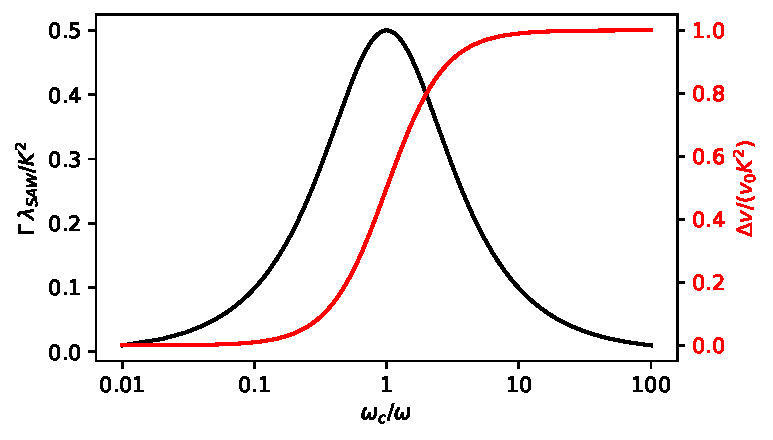
\includegraphics[width=0.8\textwidth]{gamma_and_v.pdf}
    \caption{Eq.\ \ref{gamma_bulk} (left axis) and Eq.\ \ref{v_bulk} (right axis) plotted as dimensionless quantities against the ratio $\omega_c/\omega$.}
    \label{gamma_and_v}
\end{figure}
Equations \ref{v_bulk} and \ref{gamma_bulk} are known as the "classical relaxation model" for the acoustoelectric effect. Equation \ref{v_bulk} describes relaxation dispersion, which is common in other acoustic systems \cite{hutson_elastic_1962, rudenko_dispersive_2022} and can be understood as follows: First, the SAW strains the piezoelectric, perturbing the material from its equilibrium state. Then, the piezoelectric relaxes to equilibrium, returning energy to the SAW after a time $1/\omega_c$. However, depending on the time delay between stimulus ($1/\omega$) and response ($1/\omega_c$), this energy returns to the SAW with a phase delay, leading to dispersion and attenuation. In our case, the relaxation time (and thus, $\omega_c$) depends on the conductivity of the piezoelectric semiconductor. 

\subsection{Surface acoustic waves propagating in two-dimensional materials} \label{SAW theory, propagating in 2D materials}

Equation \ref{gamma_bulk} is fundamental to our investigations into acoustoelectric charge pumping in Ch.\ \ref{AE charge pumping paper}. However, Eqs.\ \ref{v_bulk} and \ref{gamma_bulk} describe a bulk piezoelectric material with conductivity $\sigma$. How do these relations change when the conductivity is located in a thin film on an insulating piezoelectric material? Figure \ref{SAW in thin film} (a) shows the bulk case described by Eqs. \ref{gamma_bulk} and \ref{v_bulk}, in which the SAW's energy and the induced current is contained within a depth $1/k$ of the surface. Therefore, a thin film with sheet conductivity $\sigma_{2D}$ on an insulating piezoelectric (Fig.\ \ref{SAW in thin film} (b)) can be modelled as a semiconducting piezoelectric with bulk conductivity $\sigma_{2D}k$.

\begin{figure}
    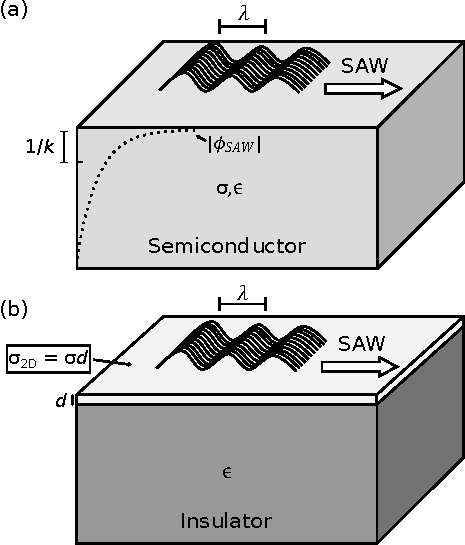
\includegraphics[width = 0.6\textwidth]{SAW in thin film.pdf}
    \caption{(a) A SAW propagating in a bulk material with conductivity $\sigma$ and permittivity $\epsilon$. (b) A SAW propagating in a piezoelectric material with permittivity $\epsilon$ that has been capped by a conductive material of thickness $d$ and sheet conductivity $\sigma_{2D} = \sigma d$.}
    \label{SAW in thin film}
\end{figure}

Consider the scenario where the current-carrying region, initially having a thickness of $1/k$, is compressed into a thin layer of thickness $d$. This thin layer has a sheet conductivity $\sigma_{2D} = \sigma d$ (here, I assume that $d \ll 1/k$). When the thickness of the current-carrying region is reduced from $1/k$ to $d$, its conductance decreases by a factor of $1/kd$. Consequently, in the 2D case, the dielectric relaxation frequency is also reduced by a factor of $1/kd$. This results in a new expression for the dielectric relaxation frequency, 

\begin{equation}
    \omega_c = \frac{\sigma_{2D}k}{\epsilon}.
\end{equation}
Next, the ratio $\omega_c/\omega$ becomes

\begin{equation}
    \frac{\omega_c}{\omega} = \frac{k\sigma_{2D}}{\epsilon}\frac{1}{\omega} = \sigma_{2D}\frac{k}{\omega \epsilon} = \frac{\sigma_{2D}}{\sigma_M}, \label{omega_c div omega}
\end{equation}
where $\sigma_M = v \epsilon$ is defined as the "characteristic conductivity" of the dielectric environment surrounding the 2D material. Finally, Eqs. \ref{v_bulk} and \ref{gamma_bulk} can be modified using Eq.\ \ref{omega_c div omega}, resulting in 

\begin{equation}
    \frac{\Delta v}{v_0} = \frac{K^2}{2}\frac{1}{1+(\sigma_{2D}/\sigma_M)^2} \label{v_2D}
\end{equation}
and
\begin{equation}
    \Gamma = K^2 \frac{\pi}{\lambda}\left(\frac{(\sigma_{2D}/\sigma_M)}{1+(\sigma_{2D}/\sigma_M)^2}\right). \label{gamma_2D}
\end{equation}
Similarly to the bulk case, in the thin film scenario, the SAW is dispersing and losing energy as it interacts with the conductive thin film. However, the attenuation and dispersion are frequency-independent, and depend only on the ratio $\sigma_{2D}/\sigma_M$. This raises a significant question: Where does the lost SAW energy go? 


\subsection{The 2D acoustoelectric charge pumping effect} \label{classical relaxtion model}

Fal'ko and Iordanskii found that the oscillating electric field that co-propagates with the SAW imparts an effective force on charge carriers. When this electric field passes through a thin film, it drives a DC sheet current that is proportional to the attenuation $\Gamma$ \cite{falko_acoustoelectric_1993}. In this section, I present the sketch of Fal'ko and Iordanskii's model given in Ref.\ \cite{esslinger_ultrasonic_1994}, which is more accessible than the original derivation (Ref.\ \cite{falko_acoustoelectric_1993}). As previously discussed, a SAW is accompanied by a co-propagating piezoelectric field of the form\footnote{Note that when a quantity such as $E(x,t)$ or $j(x,t)$ is complex, the physical observable is given by the real part.}

\begin{equation}
    E_p(x, t) = E_0 \mathrm{e}^{i(kx - \omega t)}. \label{SAW plane wave}
\end{equation}
The mobile electrons in the thin film screen this field based on the local conductivity $\sigma$, resulting in an effective field

\begin{equation}
    E(x,t) = E_p(x,t) + E_{ind}(x,t) = \frac{E_p(x,t)}{1+i(\sigma_{2D}/\sigma_M)}, \label{E eff}
\end{equation}
where $E_{ind}$ is the induced screening field, and $E_{ind}$ is phase-shifted with respect to $E_p(x,t)$ by $\phi = \mathrm{arctan}(\sigma_{2D}/\sigma_M)$.
This effective electric field creates a local oscillating current density

\begin{equation}
    j(x,t) = \sigma_{2D} E(x,t), \label{2D AE ohm's law}
\end{equation}
where $\sigma_{2D}$ is the sheet conductivity of the thin film, and $j(x,t)$ is a sheet current with dimensions of current/length. Assuming that the amplitude of the perturbation in electron density caused by the SAW (denoted by $\Delta n$) is much smaller than the average electron density in the thin film (denoted by $n_0$), the periodic electron density in the SAW takes the form\footnote{If $\Delta n \geq n_0$, the perturbation in $n$ can not be approximated as local, leading to the nonlinear acoustoelectric effect. I discuss this further in Sec.\ \ref{nonlinear acoustoelectric effect}.}


\begin{equation}
    n(x,t) = n_0 + \Delta n(x,t). 
\end{equation}
Using the continuity equation $\pdv*{J}{x} = q \pdv*{n}{t}$, $\Delta n$ can be written in terms of $E(x,t)$, giving

\begin{equation}
    \Delta n(x,t) = -\frac{\sigma_{2D}}{q} \frac{k}{\omega} E(x,t) = -\frac{\sigma_{2D}}{q} \frac{1}{v}E(x,t). \label{delta n modified}
\end{equation}

At this point, from Eqs. \ref{delta n modified} and \ref{E eff}, we can predict how the pumped acoustoelectric current will depend on the ratio $\sigma_{2D}/\sigma_M$. Figure \ref{piezoelectric field and delta n} shows $n(x,0)$ and $E_p(x,0)$ for different limiting cases of $\sigma_{2D}/\sigma_M$. If $\sigma_{2D} \gg \sigma_M$ (the film is a perfect conductor), $E_{ind}(x,t)$ = $-E_p(x,t)$, giving an effective field $E(x,t)$ = 0, and $n(x,t) = n_0$ (Eq.\ \ref{delta n modified}). This makes sense, as a perfect conductor can completely screen out the piezoelectric fields $E_p(x,t)$. If $\sigma_{2D} \ll \sigma_M$, $E(x,t)$ is perfectly in phase with $n(x,t)$. Thus, the piezoelectric field $E_p(x,t)$ pushes equal magnitudes of charge in either direction, and there can be no net current. Finally, if $\sigma_{2D} = \sigma_M$, $E_p(x,t)$ and $n(x,t)$ are out of phase such that the maximal charge density always lies on the front edge of the co-propagating SAW electric field. Therefore, $E_p(x,t)$ will always push a greater magnitude of charge in the direction of the SAW, resulting in a net current.


%TODO: Add SAW direction of travel to this figure

\begin{figure}
    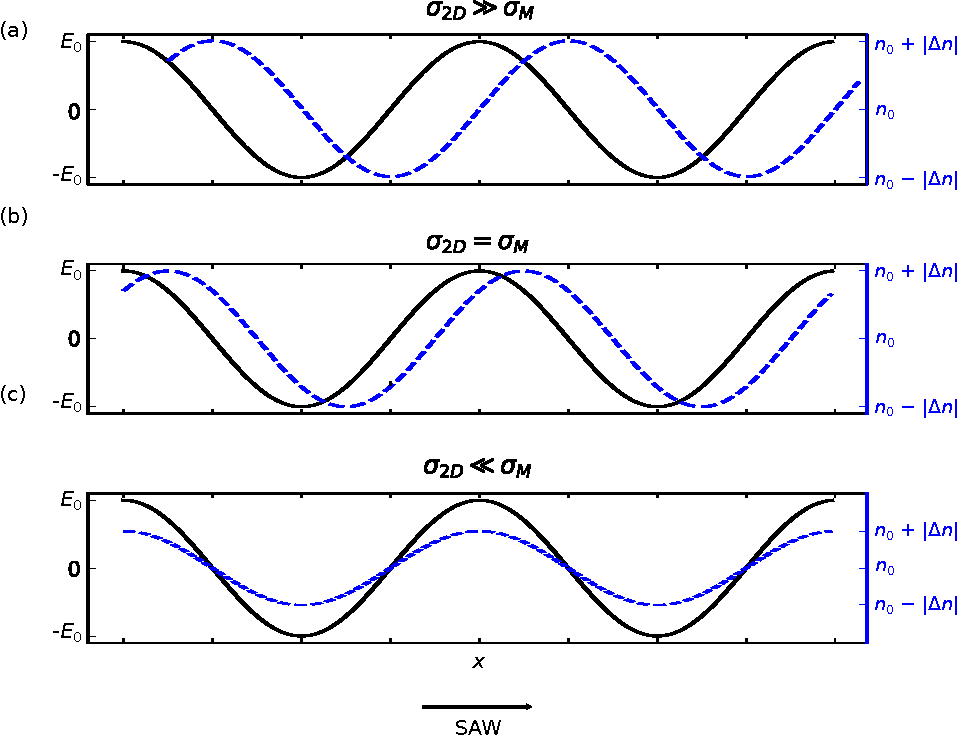
\includegraphics{piezoelectric field and delta n edited.pdf}
    \caption{Real part of $E_p$ (left axis) and $\Delta n$ (right axis) plotted for the case of (a) $\sigma_{2D} \gg \sigma_M$ (very high sheet conductivity), (b) $\sigma_{2D} = \sigma_M$, and (c) $\sigma_{2D} \ll \sigma_M$ (very low sheet conductivity).}
    \label{piezoelectric field and delta n}
\end{figure}

To find an expression for the acoustoelectric current density, we can determine how $n(x,t)$ varies with $\sigma_{2D}$ and plug that relation into Eq.\ \ref{2D AE ohm's law}. With $\Delta n \ll n_0$, and remembering that $\sigma_{2D} = q n \mu$, the time-varying sheet conductivity $\sigma(x,t)$ takes the form

\begin{equation}
    \begin{split}
        \sigma(x,t) = \sigma_0 + \pdv{\sigma_{2D}}{n} \Delta n(x,t) = \sigma_0 + (q \mu)(\frac{-\sigma_{2D}}{q} \frac{1}{v}E(x,t)) \\
        = \sigma_0 - \frac{\mu \sigma_{2D}}{v}E(x,t),
    \end{split}
    \label{sigma modified}
\end{equation}
where $\sigma_0$ is the average sheet conductivity caused by an electron density $n_0$. Now, we can find the DC acoustoelectric current by plugging Eqs. \ref{sigma modified} and \ref{delta n modified} into \ref{2D AE ohm's law} and taking the time average, giving

\begin{equation}
    \begin{split}
        j(x) = \left\langle j(x,t) \right\rangle = \left\langle \sigma(x,t) E(x,t) \right\rangle \\
        = \left\langle \left( \sigma_0 - \frac{\mu \sigma_{2D}}{v}E(x,t) \right) E(x,t)  \right\rangle \\
        = - \frac{\mu}{v}\left\langle\sigma_{2D} E(x,t)^2\right\rangle. 
    \end{split}
    \label{j time averaged}
\end{equation}
One might initially consider the notion of an oscillating $E$-field creating a DC current to be counter-intuitive. However, we can now see that, though $\left\langle E(x,t) \right\rangle = 0$, a DC current arises from the cross-term $\left\langle \sigma E(x,t) ^2 \right\rangle$, which corresponds to the time-averaged Ohmic power dissipated by the charge carriers in the thin film. So far, this model considers a local perturbation in $n$ from the SAW; therefore, this cross-term can be thought of as the local dissipation of SAW power by charge carriers in response to the co-propagating electric field. 
%TODO: Make subscripts which are not variables not italics

Finally, we can relate Eq.\ \ref{j time averaged} to $\Gamma$ to get $j$ in terms of $\sigma_{2D}/\sigma_M$. Remembering that $\Gamma$ describes the loss in SAW intensity per unit length, the SAW intensity $I$ can be written in the form

\begin{equation}
    I(x) = I_0 \mathrm{e}^{(-\Gamma x)}.
\end{equation}
Rearranging and differentiating $I$ with respect to $x$, $\Gamma$ takes the form

\begin{equation}
    \Gamma = \frac{1}{I} \pdv{I}{x} = \frac{1}{I}\left\langle\sigma E(x,t)^2\right\rangle. \label{gamma time averaged}
\end{equation}
Then, combining Eqs. \ref{j time averaged} and \ref{gamma time averaged}, the DC acoustoelectric current density becomes

\begin{equation}
    \begin{split}
        j = - \frac{\mu}{v}\left\langle\sigma E(x,t)^2\right\rangle = - \frac{\mu}{v} I\Gamma = - \frac{\mu I}{v} \frac{K^2}{2\lambda}(\frac{(\sigma_{2D}/\sigma_M)}{1+(\sigma_{2D}/\sigma_M)}). \
    \end{split}
    \label{DC AEC electron case}
\end{equation}
The above derivation assumes that the thin film is populated only by electrons. If the thin film is populated by holes, the continuity equation is instead $\pdv*{J}{x} = -q \pdv*{n}{t}$. Thus, the sign of Eq.\ \ref{delta n modified} is reversed, giving

\begin{equation}
    \Delta p(x,t) = \frac{\sigma_{2D}}{q} \frac{1}{v}E(x,t)
\end{equation}
for the local oscillating hole density. The conductivity is still given by $\sigma_{2D} = q p \mu$ (does not flip sign), resulting in

\begin{equation}
    \sigma(x,t)= \sigma_0 + \frac{\mu \sigma_{2D}}{v}E(x,t)
\end{equation}
for the time-varying sheet conductivity in the hole-transport case. Finally, the DC acoustoelectric current density for hole transport becomes

\begin{equation}
    j = \frac{\mu I}{v} \frac{K^2}{2\lambda}(\frac{(\sigma_{2D}/\sigma_M)}{1+(\sigma_{2D}/\sigma_M)}). \label{DC AEC hole case}
\end{equation}
Comparing Eqs. \ref{DC AEC electron case} and \ref{DC AEC hole case}, they are identical, but have opposite sign. A right-moving hole and right-moving electron produce the same magnitude of conventional current, but with the opposite sign. Therefore, the SAW pushes both electrons and holes in the same direction. This is in stark contrast to ordinary DC current, where electrons and holes move in opposite directions under a DC electric field, resulting in the same sign of conventional current for electron and hole transport.

Equations \ref{v_2D}, \ref{gamma_2D}, \ref{DC AEC hole case}, and \ref{DC AEC hole case} are central to interactions between SAWs and quantum materials. However, they do not consider mixed-carrier transport, where both electrons and holes are present; for example, in graphene near the charge neutrality point. In Sec.\ \ref{AE paper discussion}, we modify this classical relaxation model, which assumes charge carriers of a single type, to describe mixed-carrier transport in graphene.


\section{Surface acoustic wave device design} \label{SAW device design}

So far, I have described the propagation of surface acoustic waves (SAWs), and how they interact with charge carriers in thin films; however, I have not discussed how SAWs are generated. In this section, I first present the equations for the frequency response and impedance of a SAW device, which are derived from the point source and equivalent circuit models respectively. These are the equations which inform the design of the SAW devices used in Ch.\ \ref{AE charge pumping paper}. Next, I discuss the effect of IDT geometry on SAW device impedance, which I use to inform my design of SAW devices throughout this dissertation. I put particular emphasis on designing the geometry of IDTs (features such as the number of finger pairs and aperture width) to best match the impedance of an RF signal generator. At the end of this section, I briefly summarize these design rules which ensure well-performing SAW devices. The discussion in this section follows that of Chapters 3 and 4 of Ref.\ \cite{campbell_surface_1989}. I also found Refs.\ \cite{datta_surface_1986,lane_integrating_2021} immensely helpful in my initial stages of learning about SAW device design.

\subsection{Model for frequency-dependent response of interdigitated transducers}

SAWs are generated by interdigitated transducers, or IDTs. IDTs consist of pairs of interdigitated electrodes, or "fingers", which convert an RF signal into SAWs, or SAWs into an RF signal. Figure \ref{SAW diagram} (a) shows a schematic of an IDT. An RF signal is applied such that adjacent fingers have opposite polarity. The wavelength $\lambda$ of the generated SAW spans two fingers of the IDT. Because of this, one of the defining parameters of an IDT is the number of finger pairs $N_p$. 

The electrical response of an IDT can be approximated by assuming that each IDT finger is an infinitely thin point source separated from the adjacent finger by $\lambda/2$. This is known as the "point source model" or "delta function model". The frequency response (or "transfer function") of a single IDT in the delta function model can be approximated as \cite{campbell_surface_1989}

\begin{equation}
    \begin{split}
        H(f) = \frac{V_{in}}{V_{out}} = N_p \abs{\frac{\sin (N_p \pi (f-f_0) / f_0)}{N_p \pi (f-f_0) / f_0}},
    \end{split}
    \label{Response of IDT}
\end{equation}
where $V_{in} = \sqrt{P_{\mathrm{RF}}}$ is the amplitude of the input RF signal, $V_{out} = \sqrt{P_{SAW}}$ is the amplitude of the output SAW, and $f_0 = v/\lambda$ (where $v$ is the SAW velocity) is the center frequency of the IDT. Figure \ref{SAW diagram} (b) shows Eq.\ \ref{Response of IDT} for various values of $N_p$. 

From Eq.\ \ref{Response of IDT}, we can glean two important characteristics of the frequency response of an IDT: First, the maximum conversion of input RF power to SAW power occurs at the center frequency $f_0$. Second, as $N_p$ increases, a higher proportion of input RF power is converted to SAW power and the central bandwidth of the IDT decreases. Figure \ref{SAW diagram} (b) shows $H(f)$ for $N_p = 5$ and $N_p$ = 10.

\begin{figure}
    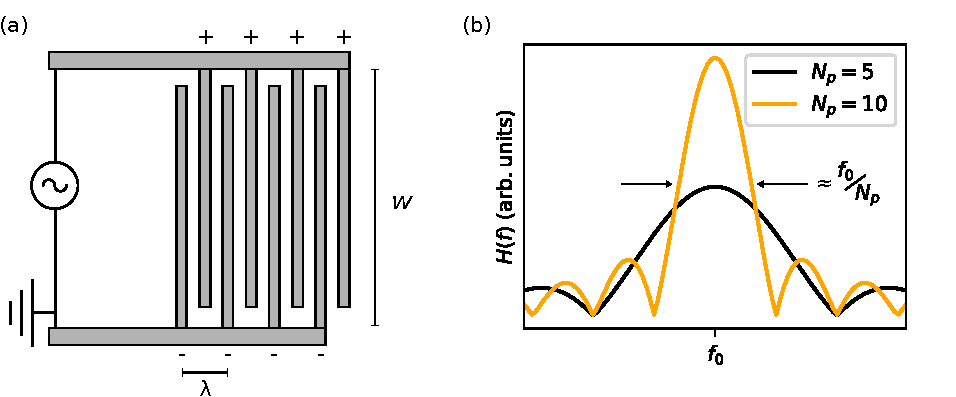
\includegraphics{SAW diagram.pdf}
    \caption{(a) Schematic of an IDT with aperture width $w$. A SAW is generated by applying an RF voltage across the interdigitated fingers. (b) Comparison between IDT response $H(f)$ for IDTs with $N_p = 5$ and $N_p = 10$. The full width at half maximum of $H(f)$ is $\approx f_0/N_p$.}
    \label{SAW diagram}
\end{figure}


\subsection{Estimating the impedance of interdigitated transducers}

It is desirable to minimize the loss between RF power applied to the SAW device and output SAW power. For example, in the experiments described in Ch.\ \ref{AE charge pumping paper}, a higher output SAW power results in a larger acoustoelectric signal. 

The largest loss between input RF power and output SAW power arises from RF power reflected back from the IDT due to an impedance mismatch between the RF signal generator and IDT, which I will refer to as "insertion loss". To estimate insertion loss, we can represent the SAW device as an arbitrary load with complex impedance $Z_{\mathrm{IDT}} = R_{IDT} + i\chi_{IDT}$, where $R_{\mathrm{IDT}}$ and $\chi_{\mathrm{IDT}}$ are the real (also known as resistive) and imaginary (also known as reactive) parts of the load impedance. Figure \ref{transmission line} illustrates a load with impedance $Z_{\mathrm{IDT}}$ driven by an ideal RF signal generator with purely real input impedance $R_{\mathrm{in}}$.


\begin{figure}
    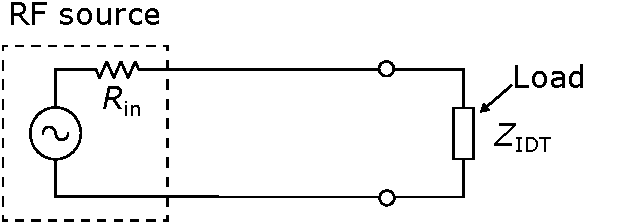
\includegraphics{IDT signal line model.pdf}
    \caption{To estimate the ratio between applied RF power and resultant SAW power, we can model the IDT as a load with complex impedance $Z_{\mathrm{IDT}}$ driven by an ideal RF signal generator with purely real input impedance $R_{\mathrm{in}}$.}
    \label{transmission line}
\end{figure}
The reflection coefficient, $\gamma$, represents the ratio of input RF power to reflected power $P_{\mathrm{in}}/P_{\mathrm{r}}$. $\gamma$ is dependent on the RF source impedance, $R_{in}$, and load impedance, $Z_{IDT}$, and for a purely real source impedance is given by \cite{kurokawa_power_1965}

\begin{equation}
    \gamma = \frac{P_{\mathrm{in}}}{P_{\mathrm{r}}} = \frac{Z_{\mathrm{IDT}} - R_{\mathrm{in}}}{Z_{\mathrm{IDT}} + R_{\mathrm{in}}}.
    \label{reflection coefficient}
\end{equation}
Most RF signal generators are designed with a purely real input impedance of $R_{\mathrm{in}} = \SI{50}{\ohm}$. Therefore, to minimize the reflection of RF power due to impedance mismatch, our IDTs need to be carefully designed with an impedance which is close to $Z_{IDT} = \SI{50}{\ohm}$. Moreover, the IDT impedance must be dominated by its real part. The reflection coefficient of a signal injected by a purely resistive (real) source impedance into a purely reactive (imaginary) IDT load impedance is $\gamma = 1$ (100\% of power is reflected).

The impedance of an IDT depends on its geometry, and must be found numerically. This problem has been considered by numerous other authors (for example, Ref.\ \cite{smith_analysis_1969}), and is beyond the scope of this dissertation. The relevant results are as follows: An IDT can be modelled as an equivalent circuit with capacitance $C_{IDT} = w C_s N_p$; where $w$ is the aperture width, $C_s$ is the capacitance per finger pair per unit length, and $N_p$ is the number of finger pairs; real conductance $G$; and complex conductance $B$. The total complex IDT admittance $Y = 1/Z_{IDT}$ is given by 


\begin{align}
    Y(f) &= G(f) + i(B(f) + 2\pi f C_{IDT})\\
    &= G_0 \left(\frac{\sin X}{X}\right)^2 + i \left(G_0 \frac{\sin (2X) - 2X}{2X^2} + 2\pi f C_{IDT}\right), \label{IDT admittance}
\end{align}
where $X$ is given by

\begin{equation}
    X = N_p \pi \frac{f - f_0}{f_0},
\end{equation}
where $f$ is the applied RF frequency and $f_0 = v/\lambda$ is the center frequency of the IDT (where $v$ is the SAW velocity). $G_0$ is the real admittance at the center frequency, given by 

\begin{equation}
    G_0 \approx 1.3 K^2 N_p^2 2 \pi f_0 w C_s,
    \label{IDT G0}
\end{equation}
where $C_s$ is the capacitance per unit length per finger pair, and $K^2$ is the piezoelectric coupling coefficient (see Sec.\ \ref{waves in bulk piezoelectric materials}).

This model does not consider reflections. In real IDTs, each finger not only absorbs SAWs, but also reflects them. For a more accurate model that considers reflections from each IDT finger, coupling of modes analysis must be used (see Refs. \cite[p.\ 140-149]{lane_integrating_2021} and \cite[Ch.\ 4]{campbell_surface_1989}). However, the reflection coefficient of a single IDT finger is $\approx 0.1-2\%$, so Eq.\ \ref{IDT admittance} is still useful for estimating the impedance of an IDT. 

As previously mentioned, to minimize the power reflected back from our IDT due to impedance mismatch, there are two important criteria: First, we need to match our IDT impedance at $f_0$ to the RF signal generator source impedance of $R_{\mathrm{in}} = \SI{50}{\ohm}$. Second, the impedance of the IDT should be dominated by the real part. 

When $f = f_0$, Eq.\ \ref{IDT admittance} simplifies to 

\begin{equation}
    Y(f_0) = G_0 + i(2\pi f_0 C_{IDT}).
\end{equation}
Therefore, for $Y(f_0)$ to be mostly real, we need to maximize the ratio

\begin{equation}
    \frac{G_0}{2\pi f_0 C_{IDT}} = \frac{1.3 K^2 N_p^2 2 \pi f_0 w C_s}{2\pi f_0 w C_s N_p} = 1.3 K^2 N_p.
    \label{G0 compared to B0}
\end{equation}
Therefore, by designing our IDT such that $N_p > 1/K^2$, we can ensure that our IDT impedance is mostly real. For example, $K^2 = 0.05$ for LiNbO\textsubscript{3} \cite{wixforth_surface_1989}, so IDTs on LiNbO\textsubscript{3} must have $N_p > 20$.

Next, to design our IDT such that $G_0 = 1/(\SI{50}{\ohm})$, we need to estimate the capacitance per unit length per finger pair $C_s$. Figure \ref{IDT capacitance toy model} shows a schematic of a single finger pair with finger width $\lambda/2$, center-to-center spacing $\lambda$, length $w$, and thickness $h$.\footnote{For simplicity, my IDTs are designed such that the tooth width is equal to the spacing between the teeth. However, varying the ratio between the tooth width and tooth spacing has been extensively explored, and boosts device performance in some applications (see Refs.\ \cite{datta_surface_1986, campbell_surface_1989}).}
% \begin{figure}
%     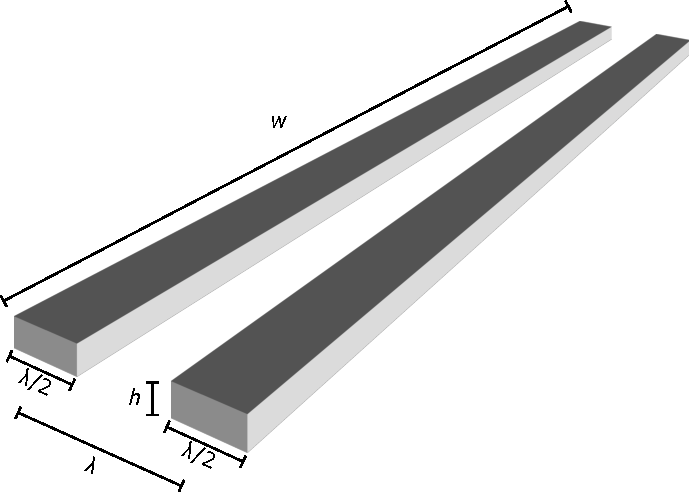
\includegraphics{IDT capacitance toy model_3d.pdf}
%     \caption{A schematic of a single finger pair with finger width $\lambda/2$, center-to-center spacing $\lambda$, length $w$, and thickness $h$.}
%     \label{IDT capacitance toy model}
% \end{figure}
% There are multiple ways to estimate the capacitance of this single finger pair. First, we could model the finger pair as two thin parallel plates separated by $\lambda$. In the parallel-plate capacitor model, the capacitance per unit length $C_s$ is

% \begin{equation}
%     C_s = \frac{\epsilon_r\epsilon_0 h}{\lambda},
% \end{equation}
% where $\epsilon_r$ is the permittivity of the space between the two plates. These fingers are sitting on a piezoelectric insulator; therefore, the effective permittivity will 

% In Sec.\ \ref{IDT methods} 

% This parallel plate model is quite coarse-grained. We also could model the fingers as two finite, cylindrical parallel wires. Using the cylindrical parallel wire model \cite[p. 682]{lonngren_fundamentals_2007}, $C_s$ is given by 

% \begin{equation}
%     C_s = \frac{\epsilon_r \epsilon_0 \pi}{\mathrm{arccosh}(\lambda/(\lambda/2))} = \frac{\epsilon_0 \pi}{\mathrm{arccosh}(2)}.
% \end{equation}
\begin{figure}
    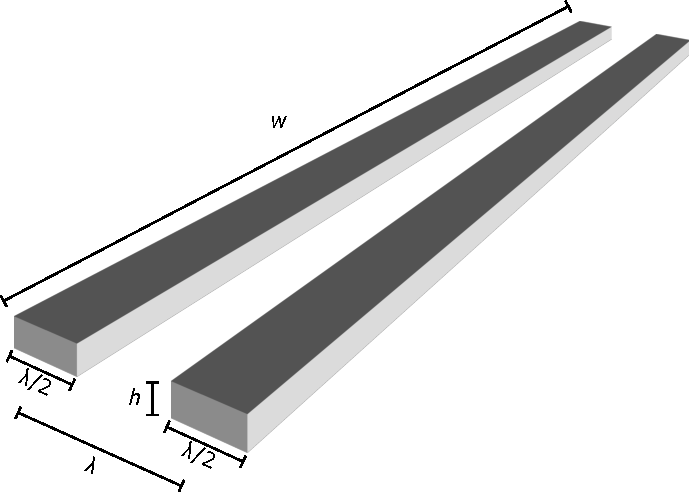
\includegraphics[width = 0.5\textwidth]{IDT capacitance toy model_3d.pdf}
    \caption{An illustration of a single finger pair with finger width $\lambda/2$, center-to-center spacing $\lambda$, length $w$, and thickness $h$.}
    \label{IDT capacitance toy model}
\end{figure}
There are multiple ways to estimate the capacitance of this single finger pair. Here, I choose to model the fingers as two finite, cylindrical parallel wires. Using a cylindrical parallel wire model \cite[p. 682]{lonngren_fundamentals_2007}, $C_s$ is given by 

\begin{equation}
    C_s = \frac{\epsilon_r \epsilon_0 \pi}{\mathrm{arccosh}(\lambda/(\lambda/2))} = \frac{\epsilon_r \epsilon_0 \pi}{\mathrm{arccosh}(2)},
    \label{IDT Cs}
\end{equation}
where $\epsilon_r$ is the relative permittivity of the dielectric part of the system. Remembering that the IDT fingers are sitting on a piezoelectric insulator, we know that the effective permittivity must be greater than $\epsilon_0$. To estimate the effective impedance of the dielectric environment around the IDT fingers, I assume that $\epsilon_r$ is the average of the permittivity of air and the permittivity of the piezoelectric substrate. For example, for LiNbO\textsubscript{3}, the relative permittivity is 85, so in Sec.\ \ref{IDT methods}, I use $\epsilon_r = (85 + 1)/2 = 43$. I use Eqs.\ \ref{IDT admittance} \textendash\ \ref{IDT Cs} in Sec.\ \ref{IDT methods} to compare this model to my measured IDT impedance (see Fig.\ \ref{Z11 plot}).

\begin{center}

    \linespread{1.0}\selectfont
    \fbox{\begin{minipage}{30em}
        Box 2.1: Designing the geometry of IDTs to minimize insertion loss.


        \begin{itemize}
            \item First, select a piezoelectric substrate. Then, to ensure that the IDT impedance is dominated by the real part, choose $N_p$ such that $N_p > 1/K^2$ (Eq.\ \ref{G0 compared to B0}). 
            \item Next, choose the designed center frequency $f_0$. Then, select $w$ such that $G_0$ (Eq.\ \ref{IDT G0}) matches the real input impedance of the RF signal generator, which is most often $1/(\SI{50}{\ohm})$.
        \end{itemize}
    \end{minipage}}

\end{center}





%-------------------------Fabrication Methods-----------------------------

\chapter{Methods} \label{methods chapter}
In this chapter, I begin by describing methods for fabricating devices from 2D materials. I first describe the best practices that I have found for exfoliation. Then, I discuss my implementation of the hot pickup method for stacking 2D materials to create heterostructures. Next, I describe the use of a highly-adhesive polymer stamp to remove unwanted 2D flakes and to tear desired flakes into areas of a single thickness. I then describe my use of photolithography for making contacts to 2D materials, and how to clean metal contacts with contact-mode AFM. I conclude this chapter by describing methods for creating interdigitated transducers (IDTs), and evaluating the performance of surface acoustic wave devices by measuring their frequency-dependent response.

\section{Fabricating 2D heterostructures} \label{fabricating 2D devices}

In 2004, the 2D materials revolution was launched when Geim and Novoselov published their experiments on exfoliated graphene, which would later win them the Nobel Prize \cite{novoselov_electric_2004}. From the humble beginnings of the "scotch tape technique", the field of has matured to an immense parameter space of layered materials for us to explore. Through the advent of transfer techniques, we can combine the properties of different 2D materials by stacking them on top of each other to create designer heterostructures.

\subsection{Exfoliation of 2D crystals}

While some groups are investigating large-area 2D growth for use in the next generation of electronics \cite{quellmalz_large-area_2021}, the best devices with the lowest electrostatic disorder are still made using mechanical exfoliation \cite{xin_giant_2023}. Using sticky tape, layered crystals are cleaved 5-10 times, then transferred onto clean SiO\textsubscript{2}. Exfoliation is a simple process, but getting consistent results can be challenging due to the vast array of variables that affect the process. Different research groups, and even different members in the same group, can have vastly differing opinions on the best methods for exfoliation. Furthermore, every 2D material has different mechanical properties, so the best recipe varies widely between materials. I gained substantial knowledge on 2D material exfoliation from my visit to the Xu group at University of Washington in 2017. Since then, I have developed my best practices through trial and error. In this section, I briefly describe my best practices for exfoliating graphene and h-BN using sticky tape. At the end of this section, I collect some tips and tricks that I have learned from performing many exfoliations. For a review of exfoliation techniques and a model of the complex physics behind mechanical exfoliation, see Ref.\ \cite{islam_exfoliation_2022}.

Exfoliation begins with selecting the tape. The two most widely used tapes are Scotch® Magic™ Tape (“Scotch Tape”) and Nitto Denko SWT20+ wafer tape, (“blue tape”). The main differences between the two are as follows: Scotch tape is stickier and leaves more residue, and blue tape is less sticky and leaves less residue. While blue tape might seem like the obvious choice for the cleanest samples, in a discussion with members of the Yankowitz group at University of Washington, I learned that they still prefer Scotch tape for graphene, as they feel it gives the largest monolayer flakes. In my experience, I find that Scotch tape does work best for graphene, giving larger-area flakes than blue tape. For h-BN, I prefer to use blue tape, as the residue left by scotch tape is similar in color to the h-BN flakes.

Figure \ref{exfoliation diagram} shows an overview of the exfoliation process. The details are as follows: First, I place a bulk layered crystal (such as graphite or boron nitride) onto sticky tape. Then, the tape is folded over and peeled back at a low angle, cleaving the bulk crystal 8-10 times for graphene and 3-5 times for h-BN. The advantage of peeling at a low angle is that it minimizes the fragmentation of the bulk crystal, resulting in larger 2D flakes.

While cleaving the bulk crystal, I plasma-clean a \SI{300}{\nano\meter} SiO\textsubscript{2}/Si substrate\footnote{Different SiO\textsubscript{2} thicknesses provide better optical contrast for different materials. \SI{300}{\nano\meter} works well for graphene and h-BN \cite{bing_optical_2018}.} using a PE-50 plasma etcher with O\textsubscript{2} plasma at \SI{50}{\watt} for 1 minute. Then, I place the tape with cleaved crystals onto the plasma-cleaned SiO\textsubscript{2} substrate and rub the top of the tape with a semi-hard instrument, such as the back of a pen or an eraser, to ensure that the tape is in good contact with the substrate. Next, I heat the substrate with tape at \SI{90}{\celsius} for 5 minutes, which helps adhere the 2D flakes to the SiO\textsubscript{2} (see Fig.\ 3 D of \cite{islam_exfoliation_2022}). Finally, I peel the tape from the SiO\textsubscript{2} slowly at a low angle, cleaving flakes from the tape onto the SiO\textsubscript{2}. 


\begin{figure}
    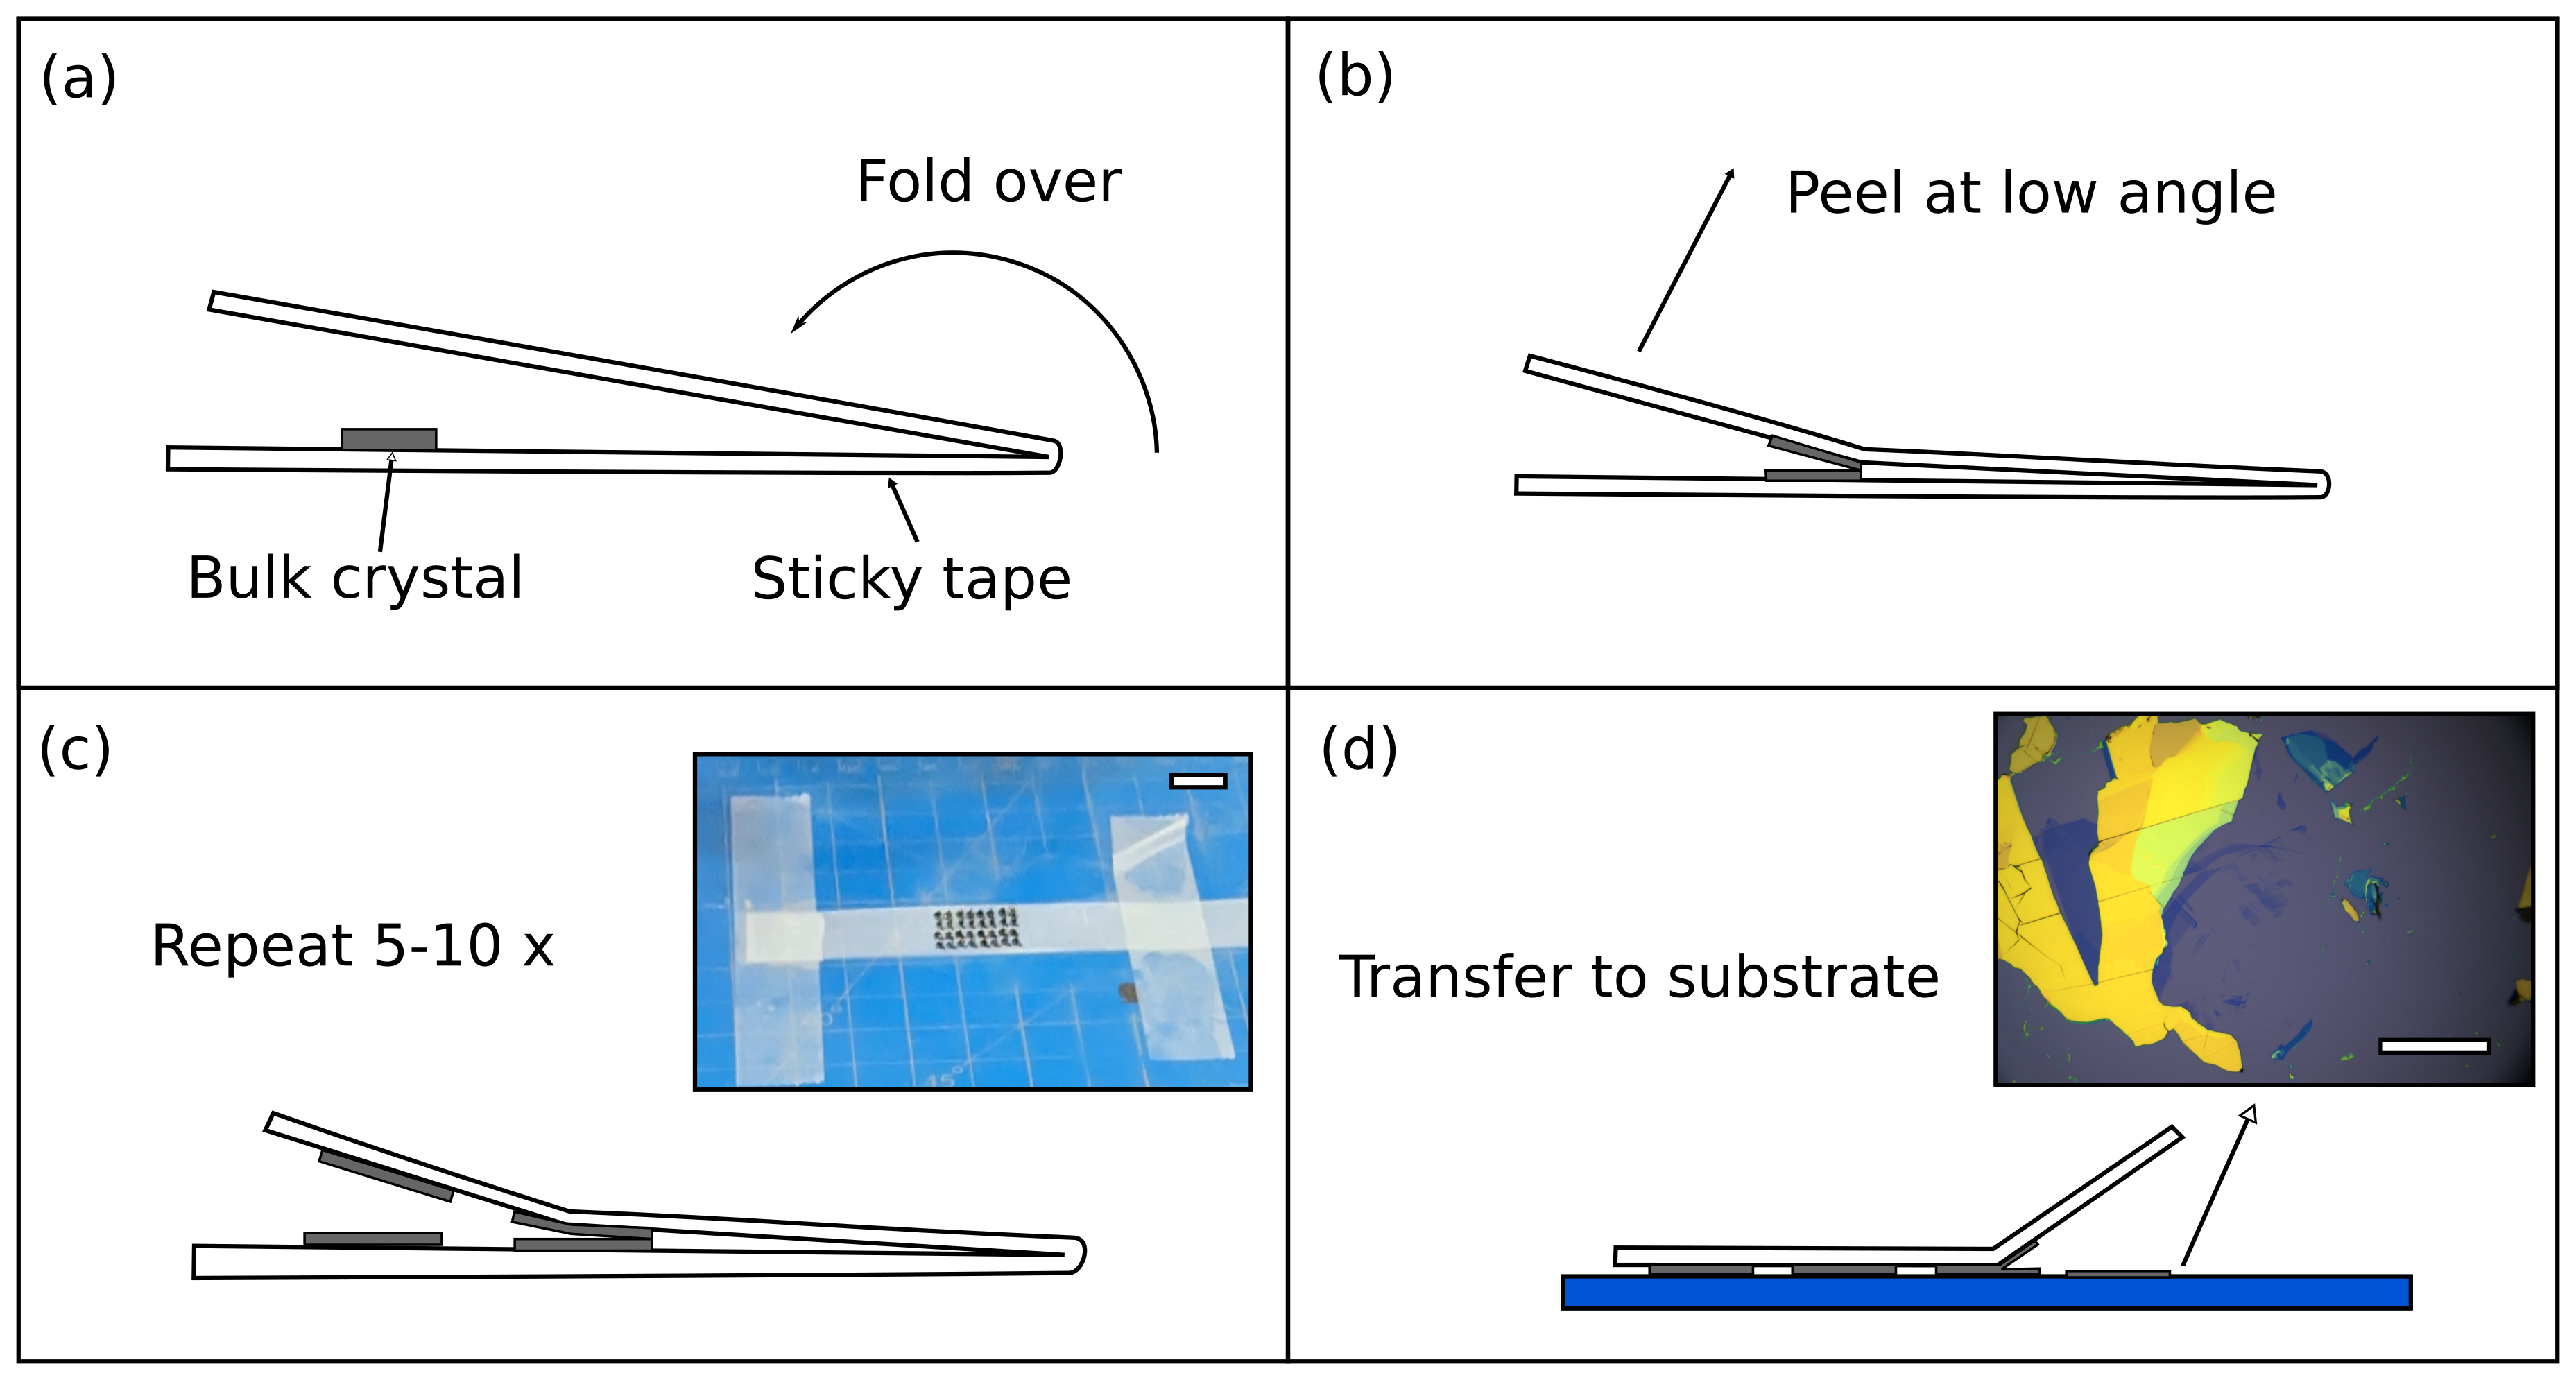
\includegraphics{exfoliation diagram.pdf}
    \caption{The process for exfoliating 2D crystals. (a) First, the bulk crystal is placed on sticky tape, and the tape is folded over onto the crystal. (b) The tape is peeled back at a low angle to exfoliate the bulk crystal. (c) Step (b) is repeated 5-10 times. The tape is folded such that the exfoliated crystal areas do not overlap. (d) The tape is placed onto an SiO\textsubscript{2} substrate, heated at \SI{90}{\celsius} for 5 minutes, then peeled off slowly at a low angle.}
    \label{exfoliation diagram}
\end{figure}
This exfoliation process results in flakes of a variety of sizes and thicknesses, from single-layer to thousands of layers (see inset of Fig.\ \ref{exfoliation diagram} (d)). The number of layers can be determined by examining the optical contrast between the 2D flakes and the surface, and confirmed with AFM. Figure \ref{fig:graphenelayer} shows a tapping-mode AFM image (a) and optical image (b) of an exfoliated graphene flake.



\begin{figure}
    \centering
    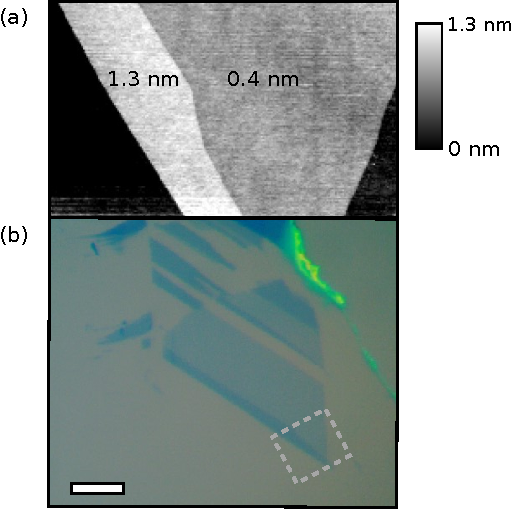
\includegraphics[width = 9cm]{graphene layer comparison.pdf}
    \caption{(a) AFM scan and (b) optical image of exfoliated graphene on SiO\textsubscript{2}. The AFM scan region is indicated by a gray dotted box. Scale bar = \SI{10}{\micro\meter}.}
    \label{fig:graphenelayer}
\end{figure}
Accurately measuring the number of layers of a graphene sample with AFM is difficult due to water layers on substrates prepared in atmospheric conditions and interactions between the AFM tip and graphene \cite{shearer_accurate_2016}. These difficulties can be reduced by using tapping-mode AFM; however, if monolayer graphene is necessary for an experiment, it is better to use Raman microscopy, which can distinguish between monolayer and multilayer graphene. In the graphene devices described in this dissertation, monolayer graphene is not imperative, so I used AFM to estimate the layer number of my graphene and h-BN samples.


\begin{center}

    \linespread{1.0}\selectfont
    \fbox{\begin{minipage}{30em}
        Box 3.1: A summary of my tips and tricks for exfoliation.


        \begin{itemize}
            \item Use scotch tape for graphene, and blue tape for h-BN
            \item Cleave 6-8 times on tape for graphene
            \item Cleave 3-5 times on tape for h-BN
            \item When peeling tape, peel at a low angle. The conventional wisdom is that this results in larger-area flakes.
            \item When placing h-BN bulk crystals onto tape, use tweezers to "smear" them flat onto the tape. h-BN crystals are thick, and need to be pressed flat to ensure good contact with the tape.
            \item Clean SiO\textsubscript{2} with O\textsubscript{2} plasma for 1 minute immediately before transferring crystals from tape onto SiO\textsubscript{2}.
            \item In the final step, anneal tape on SiO\textsubscript{2} at \SI{90}{\celsius} for 5 minutes for all materials, then cool completely (2 minutes) before peeling tape from SiO\textsubscript{2}.
        \end{itemize}
    \end{minipage}}

\end{center}



\subsection{Stacking 2D materials to create heterostructure devices} \label{transfer methods section}

The ability to isolate single layers of 2D crystals with mechanical exfoliation opened wide the possibility of stacking different atomic layers to create designer heterostructures. In 2010, Dean et al. demonstrated that the mobility and electronic disorder of graphene can be vastly improved by encapsulating the graphene in insulating hexagonal boron nitride (h-BN) \cite{dean_boron_2010}. Since then, techniques for assembling stacks of 2D materials have vastly improved, allowing for sub-micron lateral precision and sub-degree rotational alignment between layers \cite{castellanos-gomez_van_2022}. Heterostructure fabrication techniques fall into two main categories: wet-transfer methods, which use sacrificial polymer layers to place down each 2D crystal, and dry-transfer methods, which only require dissolving the polymer stamp once the entire structure is completed. In general, dry transfer methods are preferred as they reduce contamination between layers, and it is the method I use to create the devices discussed in this dissertation. Therefore, I will only describe the dry transfer method here. Different researchers have different opinions on the best tricks for 2D transfer. For an overview of different 2D transfer methods, see the review by Castellanos-Gomez et al.  \cite{castellanos-gomez_van_2022}. The methods I present in the subsequent sections were initially learned through discussions with graduate students in the University of Washington Department of Physics, then modified by me based on trial and error.

The general dry transfer process used to build 2D heterostructures is as follows: First, a sticky polymer stamp is mounted onto a micromanipulator stage (Fig.\ \ref{transfer stage image}) underneath a long-focal length microscope. The stamp is brought into contact with a chip containing exfoliated 2D flakes. The temperature of the stage is increased to make the polymer stamp stickier. Then, the contact area of the stamp on the chip is increased by lowering the stamp. Once the entire 2D flake is covered with polymer, the stage is slowly retracted to pick up the 2D flake. This process is repeated to build the desired heterostructure top-down, using the previous layer to pick up the next. Finally, the stamp is melted at a high temperature and dissolved in a solvent. This method of heating up a polymer stamp to build 2D heterostructures is called the "hot pick up technique" \cite{pizzocchero_hot_2016}.

\begin{figure}
    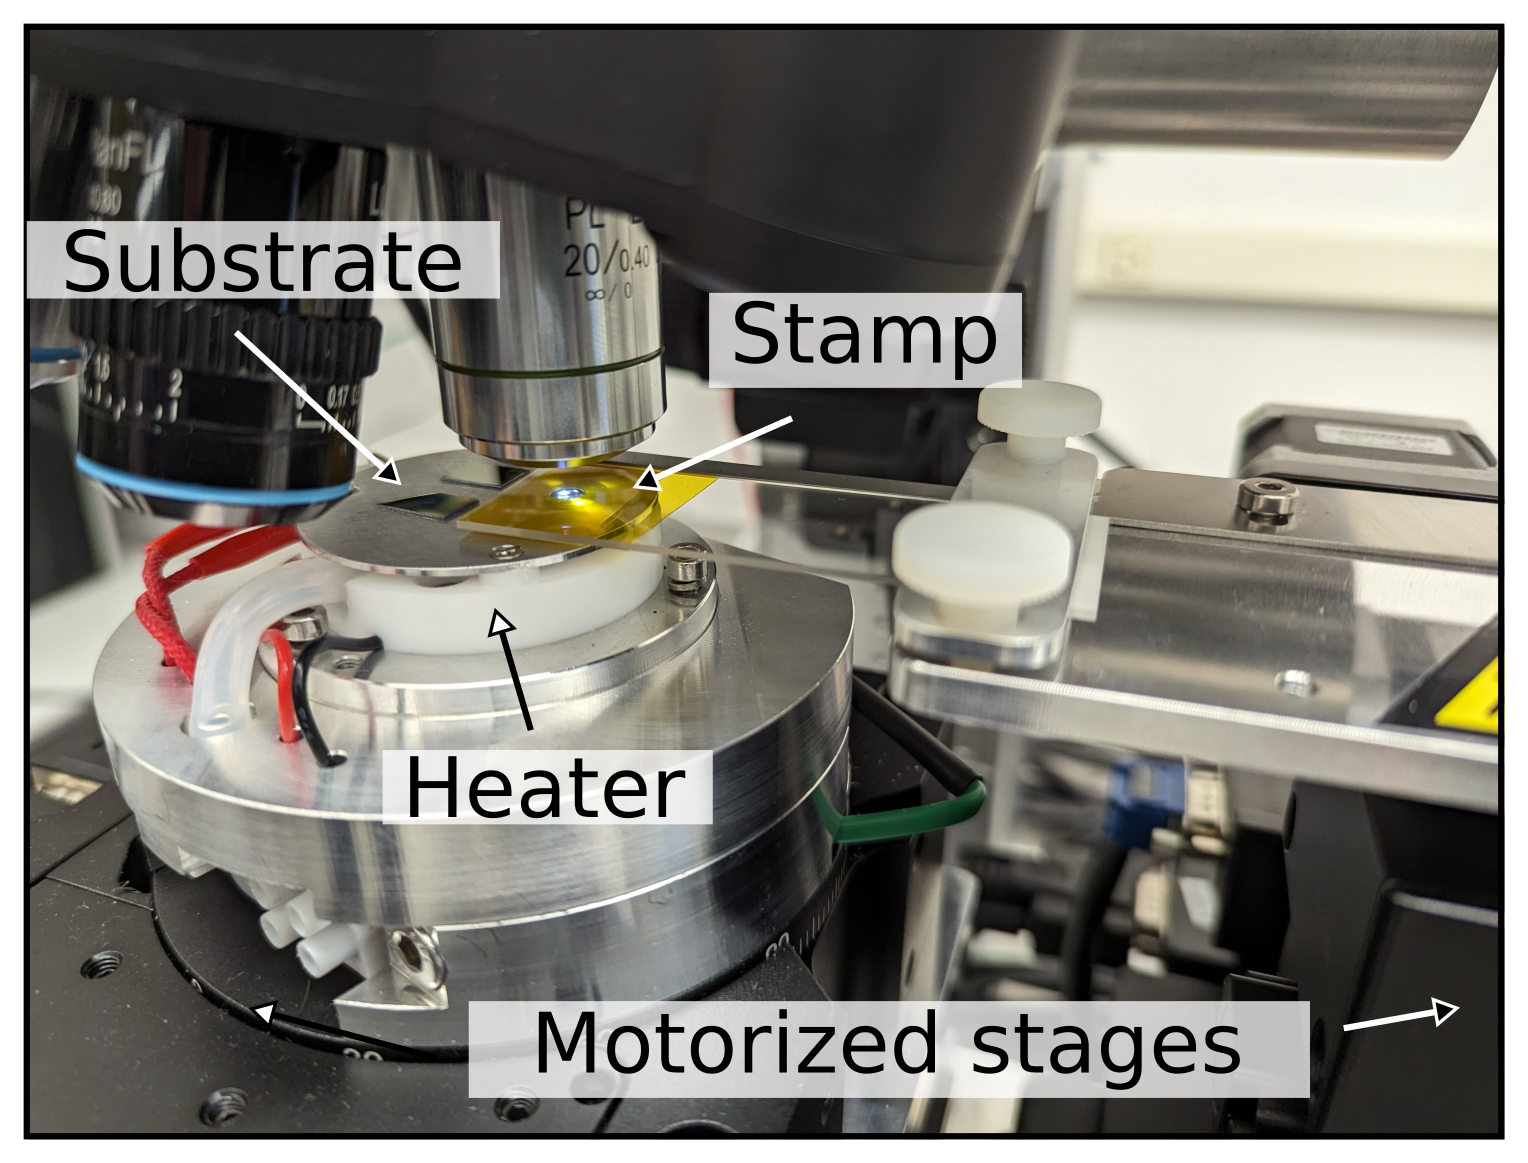
\includegraphics[width = 0.5\textwidth]{transfer stage image.pdf}
    \caption{An image of our transfer stage (purchased from HQ Graphene). A substrate containing a 2D sample is placed in-between the microscope objective and viscoelastic stamp. Using motorized stages, the stamp is used to pick up and stack 2D flakes. Heating the stage increases the stickiness of the stamp.}
    \label{transfer stage image}
\end{figure}

\subsubsection{Making the viscoelastic stamp} \label{making the PC stamp section}

Figure \ref{stamp diagram} shows the viscoelastic stamp that I use, which is used to pick up and place 2D flakes. The stamp consists of a polydimethylsiloxane (PDMS) layer mounted on a glass slide, with a thin poly(bisphenol A carbonate) (PC) polymer layer on top (some groups use polypropylene carbonate, referred to as PPC). The PDMS acts as a base for the stamp, while the PC layer becomes sticky at elevated temperatures.


\begin{figure}
    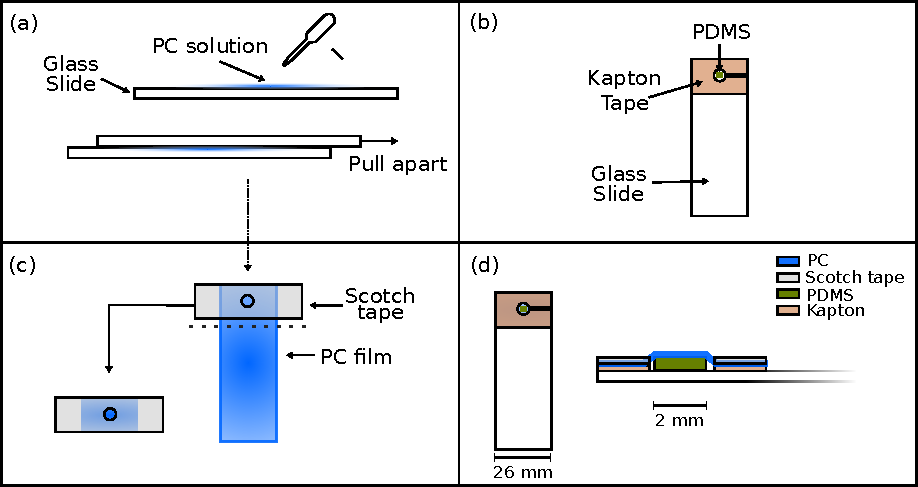
\includegraphics[width = 1\textwidth]{stamp making diagram.pdf}
    \caption{The viscoelastic stamp fabrication process. (a) First, a PC film is made by coating a glass slide with a solution of 6\% PC in chloroform, then placing another slide on top and pulling the slides apart. (b) The base of the stamp is made by punching a hole in a piece of double-sided Kapton tape, placing the Kapton on a clean slide, and placing a square of Gel-Pak PDMS on the glass slide in the center of the hole. (c) The PC film is transferred to the slide base using a piece of scotch tape with a hole punched in the center. (d) The completed viscoelastic stamp.}
    \label{stamp diagram}
\end{figure}


I build the stamp as follows: First, I prepare the PC film (Fig.\ \ref{stamp diagram} (a)) I begin by making a solution of 6\% PC in chloroform (mass percent). The PC takes 24-48 hours of stirring at medium speed to fully dissolve. Then, I clean two glass slides and place them next to each other in a fume hood. I pipette $\approx \SI{2}{\milli\liter}$ of PC solution in a line on one glass slide, then flip the other slide on top. Using light pressure, I slide the two glass slides apart, leaving a film of PC on one side of each slide. Finally, I let the slides dry for at least \SI{1}{\minute} before continuing.\footnote{The chloroform evaporates very quickly, but I usually let it dry while preparing the rest of the stamp.}

To prepare the slide that composes the base of the stamp, I use a leather punch to punch a hole in a piece of double-sided polyimide tape (Kapton). Then, I place this piece of tape on a fresh glass slide, and cut a channel in one side of the tape (Fig.\ \ref{stamp diagram} (b)). This channel allows for air to escape when placing down the PC film in the next step. Without the channel, air gets trapped between the PDMS and PC layers. Next, I take pre-made PDMS sheets (Gel-Pak) that are 17 mil (\SI{0.432}{\milli\meter}) thick. These Gel-Pak sheets have a hard backing on one side, and a soft backing on the other side. I place a strip of double-sided polyimide tape (Kapton) into a plastic dish and place a $\approx 2 \times \SI{2}{\centi\meter}$ piece of Gel-Pak sheet onto the dish, hard backing-side down. The choice to put the hard backing side down makes picking up small pieces of PDMS easier. Then, I use a clean razor blade to cut the PDMS into 2 $\times$ \SI{2}{mm} squares. Using tweezers, I remove the soft backing (on the side facing upward), grab one Gel-Pak square, and place it into the hole in the center of the mounted Kapton tape (Fig.\ \ref{stamp diagram} (b), green square).

Next, I use a leather punch with diameter $\approx  \SI{4}{\milli\meter}$ to make a hole in a piece of scotch tape. Then, I put this scotch tape down onto the dried PC film, ensuring that the area in the tape hole is clean and uniform (Fig.\ \ref{stamp diagram} (c)). I cut the PC on the edge of the scotch tape using a razor blade and pick up the PC film. Lastly, I place the PC film onto the prepared slide base, aligning the hole in the scotch tape with the hole in the Kapton tape, and press the edges of the hole to ensure good adhesion between the scotch and Kapton tapes. Figure \ref{stamp diagram} (d) shows a completed viscoelastic stamp. Before using a stamp to transfer 2D flakes, I inspect it in an optical microscope to ensure that no dust came between the PC and PDMS layers. If there is dust trapped between the layers, it can cause the two layers to de-laminate from each other. Also, 2D flakes can not be picked up near dust, as the large dust prohibits the stamp from making good contact to the 2D material. Then, I anneal the stamp at \SI{90}{C} for 5 minutes to ensure good contact between the PC and PDMS. Finally, I put the stamp in the transfer station (HQ2D MOT fully motorized transfer system from HQ Graphene) and lower it onto a bare SiO\textsubscript{2} substrate to check the location in which it first touches the surface. This determines the initial touch-down point of the stamp in the next step.


\subsubsection{The hot pickup technique for transferring 2D materials} \label{the hot pickup proces}
Figure \ref{hot pickup diagram} outlines the hot pickup process that I use for building 2D heterostructures. First, I select 2D flakes of interest using optical microscopy. Ideal flakes have a large area of a single thickness, and are free of residue (see inset of Fig.\ \ref{hot pickup diagram} (a)). I also take AFM images of flakes before I use them in a heterostructure to estimate their thickness and check for residue. 

\begin{figure}
    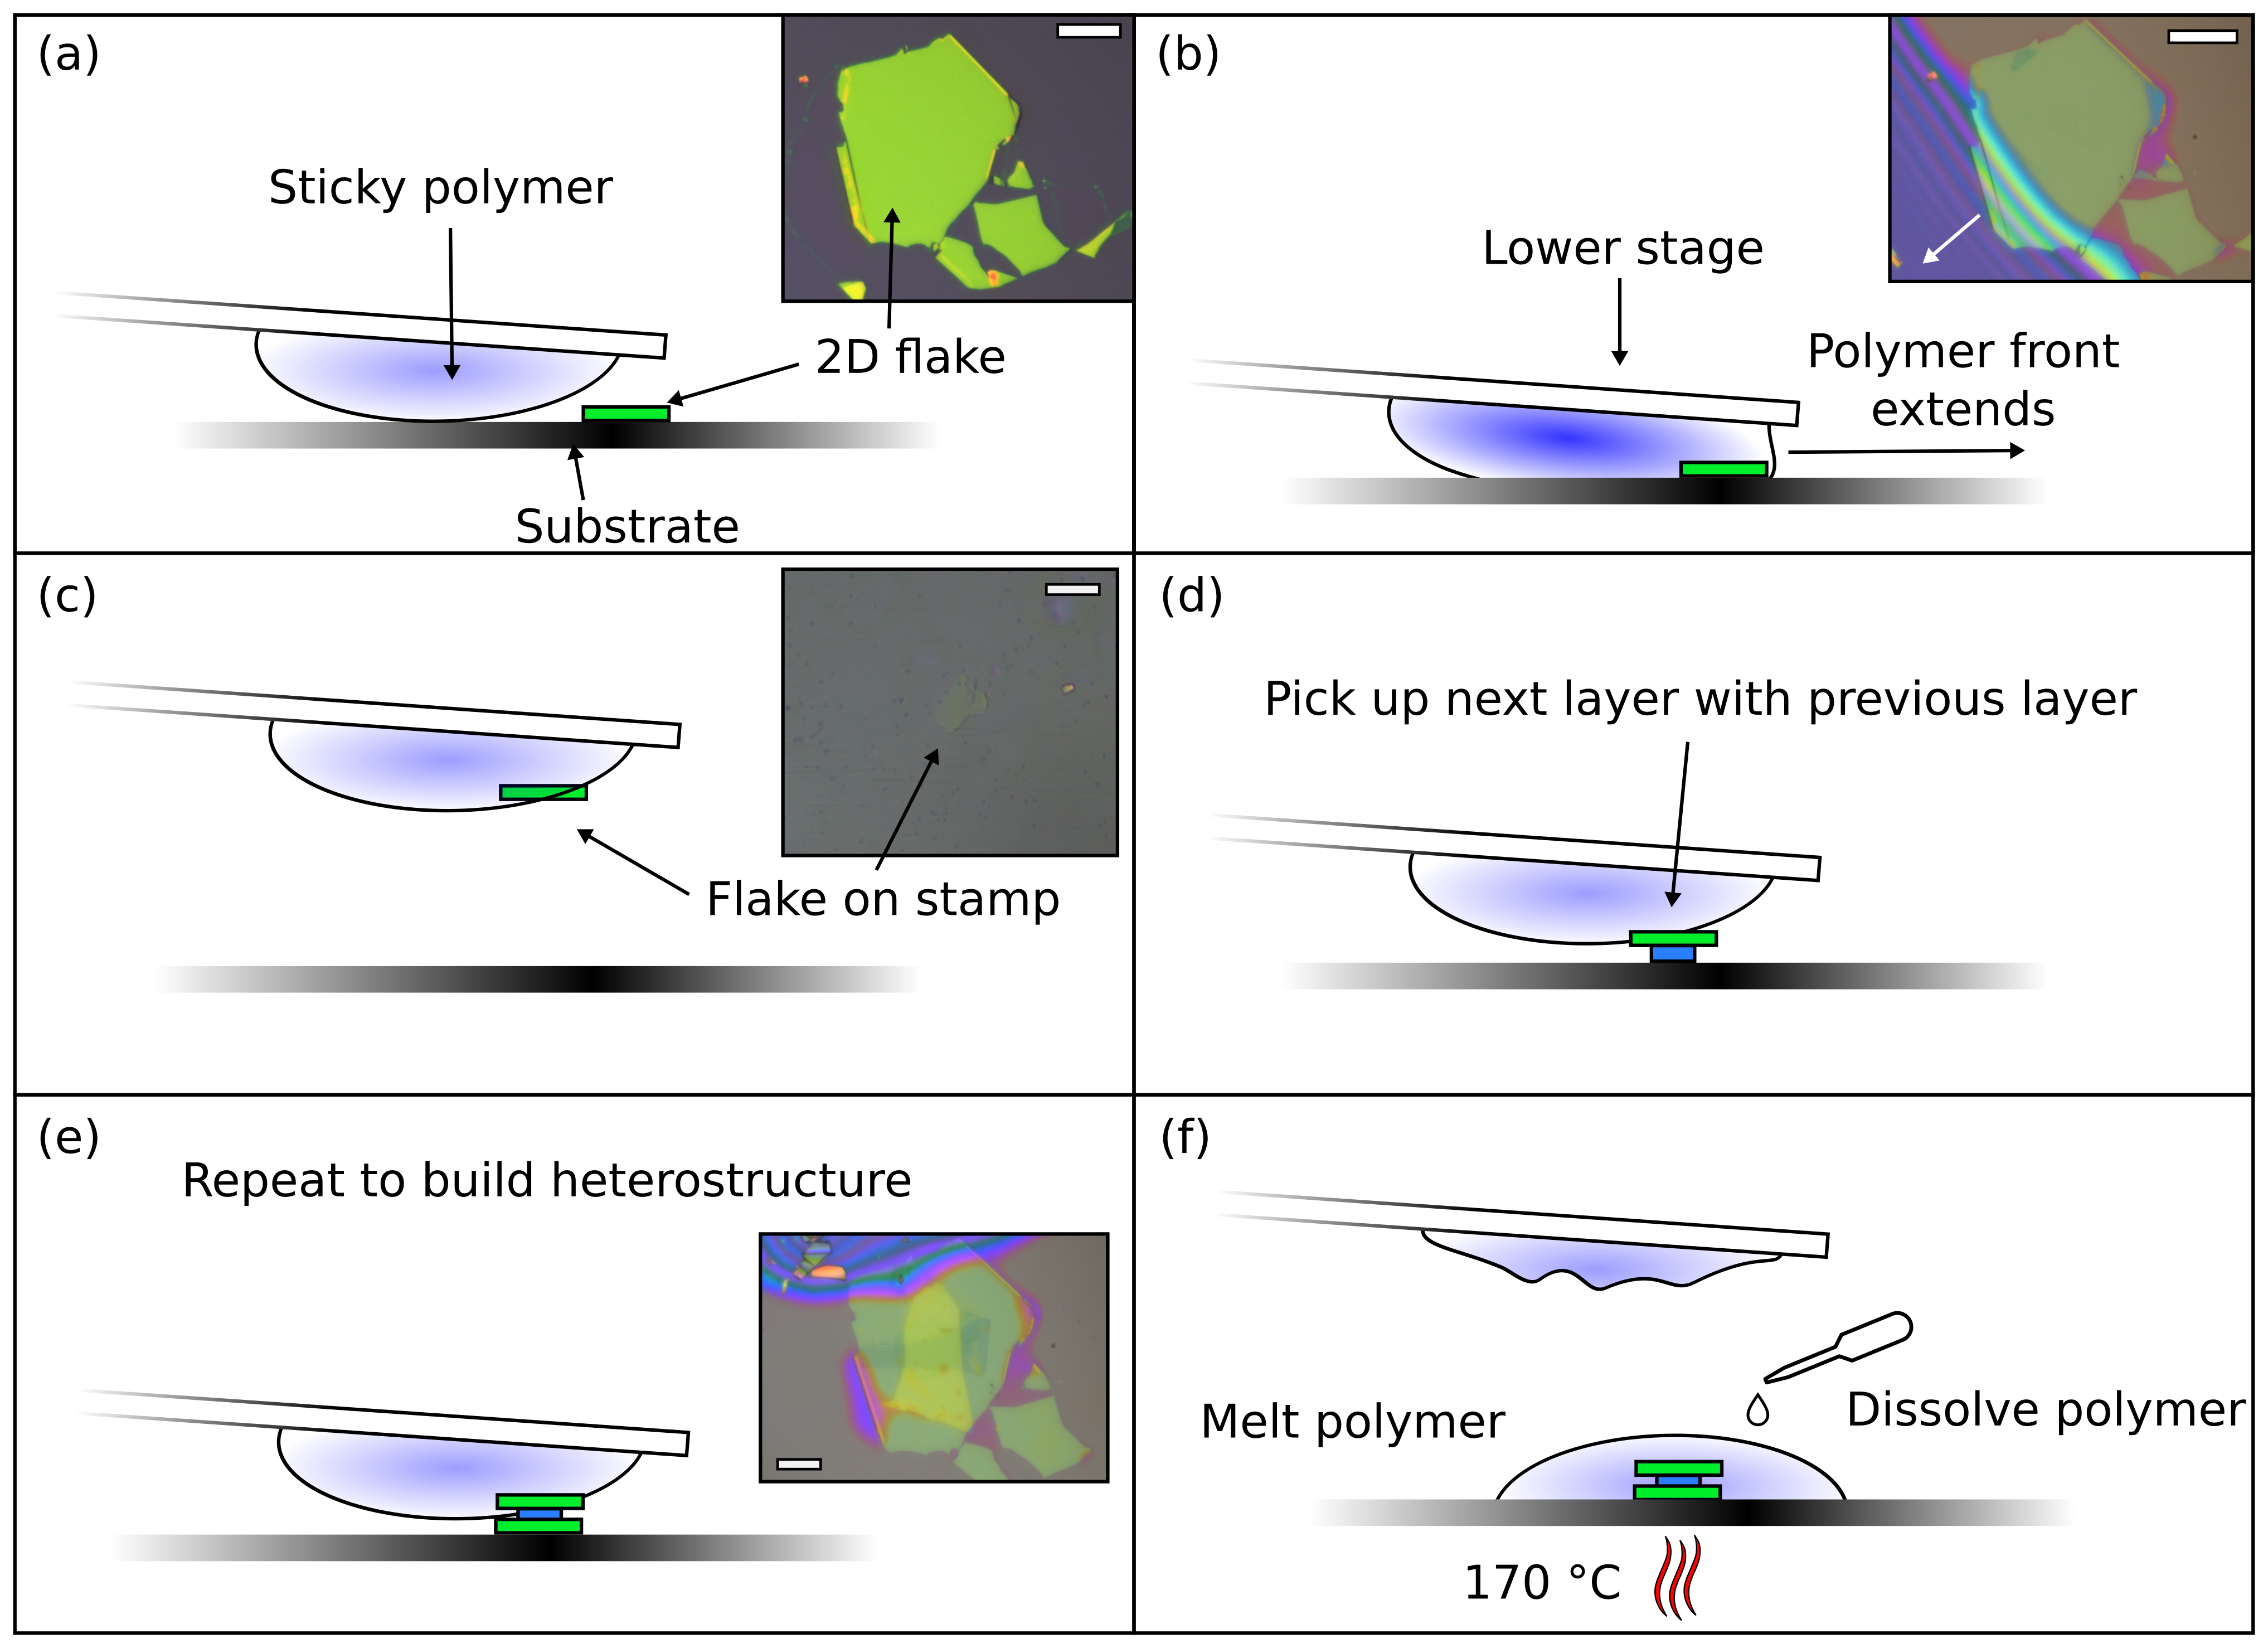
\includegraphics[width = 1\textwidth]{hot pickup diagram.pdf}
    \caption{The hot-pickup process for constructing 2D heterostructures. (a) First, the polymer stamp is lowered close to a 2D flake. Inset: a $\approx \SI{30}{\nano\meter}$ h-BN flake on SiO\textsubscript{2} (scale bar = \SI{15}{\micro\meter}). (b) The z-stage is slowly lowered and/or the stage is heated by \SI{5}{\celsius} at a time to slowly expand the polymer front over the 2D flake. Inset: a h-BN flake during the pickup process (Scale bar = \SI{15}{\micro\meter}). (c) The z-stage is slowly raised, peeling the 2D flake from the substrate. Inset: A 2D flake which has been peeled from the substrate, barely visible on a polymer stamp (Scale bar = \SI{50}{\micro\meter}). (d)-(e) Steps (a)-(c) are repeated, using the previous flake to pick up the next flake. Inset: A heterostructure composed of bottom h-BN, few-layer graphene, and top h-BN (scale bar = \SI{15}{\micro\meter}). (f) The completed heterostructure is placed down on the final substrate. The stage is heated to $\SI{170}{\celsius}$ to melt the polymer. Finally, the polymer is dissolved in a solvent.}
    \label{hot pickup diagram}
\end{figure}

I begin the transfer process by lowering the viscoelastic stamp until it touches the surface. Then, I heat up the stage to at least \SI{40}{\celsius}. The conventional wisdom is that higher temperature makes the stamp more sticky. However, high temperature also increases the likelihood of the PC and PDMS layers de-laminating (peeling away from each other), so I prefer to start at a lower temperature. For the same reason, I never heat the stage above \SI{90}{\celsius} during the transfer process. 

I then lower the z-stage until the entire 2D flake is covered by polymer. The inset of Fig.\ \ref{hot pickup diagram} (b) shows a 2D flake during the polymer expansion process. The interference fringes indicate the direction that the polymer is expanding, and the smooth surface of the portion of the flake that is covered by polymer indicates good contact between the polymer and 2D flake. It is imperative that the 2D flake is smoothly covered by polymer — if any dust or bubbles separate the flake and polymer, the flake will be difficult to pick up. After the entire flake is covered by polymer, I slowly raise the z-stage to peel the flake off of the substrate. The inset of Fig.\ \ref{hot pickup diagram} (c) shows a flake on a polymer stamp after pick-up.

Then, I find the next layer of the heterostructure and align to the previous layer by looking through the transparent polymer stamp. I then repeat the pick-up process, using the previous flake to pick up the next layer. Finally, to release the heterostructure from the stamp, I first lower the stamp onto the final substrate. Then, I heat the stage to \SI{170}{\celsius} to melt the PC away from the stamp, waiting 5 minutes to ensure that the PC is fully melted. Next, I slowly raise the stamp, ensuring that the PC pulls away from the stamp. It is important to watch the PC during this step — if the stage is too cool, the polymer will not melt enough, and the heterostructure will be picked up from the surface. Finally, I place the chip in a bath of chloroform for 20 minutes to dissolve the PC. Usually, this soak is enough to remove the PC residue. If residue needs to be cleaned off, I gently spray the edge of the chip with acetone then isopropyl alcohol, letting solvent run over the heterostructure, then dry the chip by blowing with N\textsubscript{2}. At this point, spraying the heterostructure directly with a wash bottle can release the heterostructure from the surface. After the PC is cleaned off, the heterostructure is ready for lithography (Sec.\ \ref{contacts to 2D materials}).

Exfoliation is not a deterministic process, and pristine, single-thickness areas of 2D samples often come attached to thicker areas. Also, the density of exfoliated material can be quite high, making transfer difficult. In the next section, I describe the use of a highly-adhesive stamp to clean unwanted flakes from the substrate and tear exfoliated flakes into single-thickness regions.





\begin{center}

    \linespread{1.0}\selectfont
    \fbox{\begin{minipage}{30em}
        Box 3.2: Tips and tricks for the transfer process: 


        \begin{itemize}
            \item Slowly peeling the flake from the substrate increases the success rate of the pick-up step.
            \item Higher temperatures make pick-up easier, but also increase the likelihood of ruining the stamp.
            \item Picking up thick flakes directly with the polymer stamp is easier than picking up thin flakes.
            \item Picking up subsequent flakes with h-BN is much easier than picking them up directly with the polymer.
        \end{itemize}
    \end{minipage}}

\end{center}




\subsection{Polycaprolactone (PCL) stamp for removing unwanted 2D flakes}
In this section, I describe the use of a highly-adhesive stamp to clean unwanted 2D flakes from the substrate and tear exfoliated flakes into single-thickness regions. As shown in the inset of Fig.\ \ref{exfoliation diagram} (d), thin regions of exfoliated 2D crystal often come next to thicker regions. When attempting to pick up a flake with the hot pickup method (Sec.\ \ref{transfer methods section}), a thick region will prevent good contact with an adjacent thinner region. If transfer is successful, adjacent flakes are often also picked up with the target flake. For the devices described in Ch.\ \ref{AE charge pumping paper}, an unwanted graphene flake could short-circuit the interdigitated transducer, rendering it inoperable. Therefore, this method of cleaning was necessary to successfully create the devices described in Ch.\ \ref{AE charge pumping paper}. The use of a polycaprolactone (PCL) stamp was first demonstrated in Ref.\ \cite{son_strongly_2020}, where the authors used PCL to create heterostructures with NbSe\textsubscript{2} and CrPs\textsubscript{4}. These materials have poor adhesion with h-BN and are difficult to pick up using the standard hot pick-up technique (Sec.\ \ref{the hot pickup proces}). I learned this method of PCL cleaning from the Yankowitz group at University of Washington. 

\subsubsection{Preparing the polycaprolactone stamp}


Figure \ref{PCL stamp making diagram} illustrates the process for making a polycaprolactone (PCL) stamp. The process for making a PCL stamp is very similar to the PC stamp-making process described in Sec.\ \ref{making the PC stamp section}, with two distinct differences. First, the PCL stamp uses a PCL film instead of a PC film. Second, the PDMS used is not a flat Gel-Pak sheet, but a round "dome PDMS". 

Figure \ref{PCL stamp making diagram} (a) illustrates how to make dome PDMS. First, I mix SYLGARD™ 184 Silicone Elastomer solution (PDMS solution) at a 10:1 ratio with curing agent (as per manufacturer recipe) in a plastic Petri dish with a flat bottom. I make enough curing agent to fill the dish with a $\approx \SI{2}{\milli\meter}$ layer of PDMS solution (the thickness of this layer determines the height of the dome PDMS). I then place the uncured PDMS into a vacuum chamber for 30 minutes to remove air bubbles from the PDMS solution. Then, I cure the solution on a hotplate at \SI{40}{\celsius} overnight. Next, I use a biopsy punch with diameter \SI{2.5}{\milli\meter} to punch a small, circular piece of cured PDMS out of the plastic dish and place it in a fresh plastic dish (Fig.\ \ref{PCL stamp making diagram} (a) (1)). Then, I prepare another batch of PDMS solution, and before it cures, I pipette one drop of PDMS solution onto the prepared cured PDMS piece (Fig.\ \ref{PCL stamp making diagram} (a) (2)). Due to surface tension, this droplet stays rounded on top, which defines the dome. Lastly, I cure the dome PDMS on a hot plate at \SI{40}{\celsius} overnight. Figure \ref{PCL stamp making diagram} (a) (3) shows a photo of completed dome PDMS.

To create the PCL film, I first prepare a solution of $15 \%$ polycaprolactone (PCL) in tetrahydrofuran (THF) (mass percent). I mix this solution on a stir plate at medium speed for 24-48 hours, until the PCL is fully dissolved. Then, I mount a clean glass slide on a spin-coater, and pipette $\approx \SI{2}{\milli\liter}$ of PCL solution onto the center of the slide. I then spin the solution at 2000 RPM for 1 minute. At this point, the PCL film will appear rough. Next, I melt the PCL film on a hotplate at \SI{90}{\celsius} for 1 minute, or until the PCL film becomes transparent. I then let the PCL film cool fully (until it becomes opaque again) before proceeding.

After the dome PDMS and PCL film are prepared, I construct the PCL stamp identically to the process described at the end of Sec.\ \ref{making the PC stamp section} (in this case, with dome PDMS and PCL film instead of gel-pak PDMS and PC film). In brief: I use scotch tape to transfer the PC film onto the dome PDMS, which is mounted on a glass slide (Fig.\ \ref{PCL stamp making diagram} (c) and (d)). Figure \ref{PCL stamp making diagram} shows a schematic of a completed PCL stamp.

\begin{figure}
    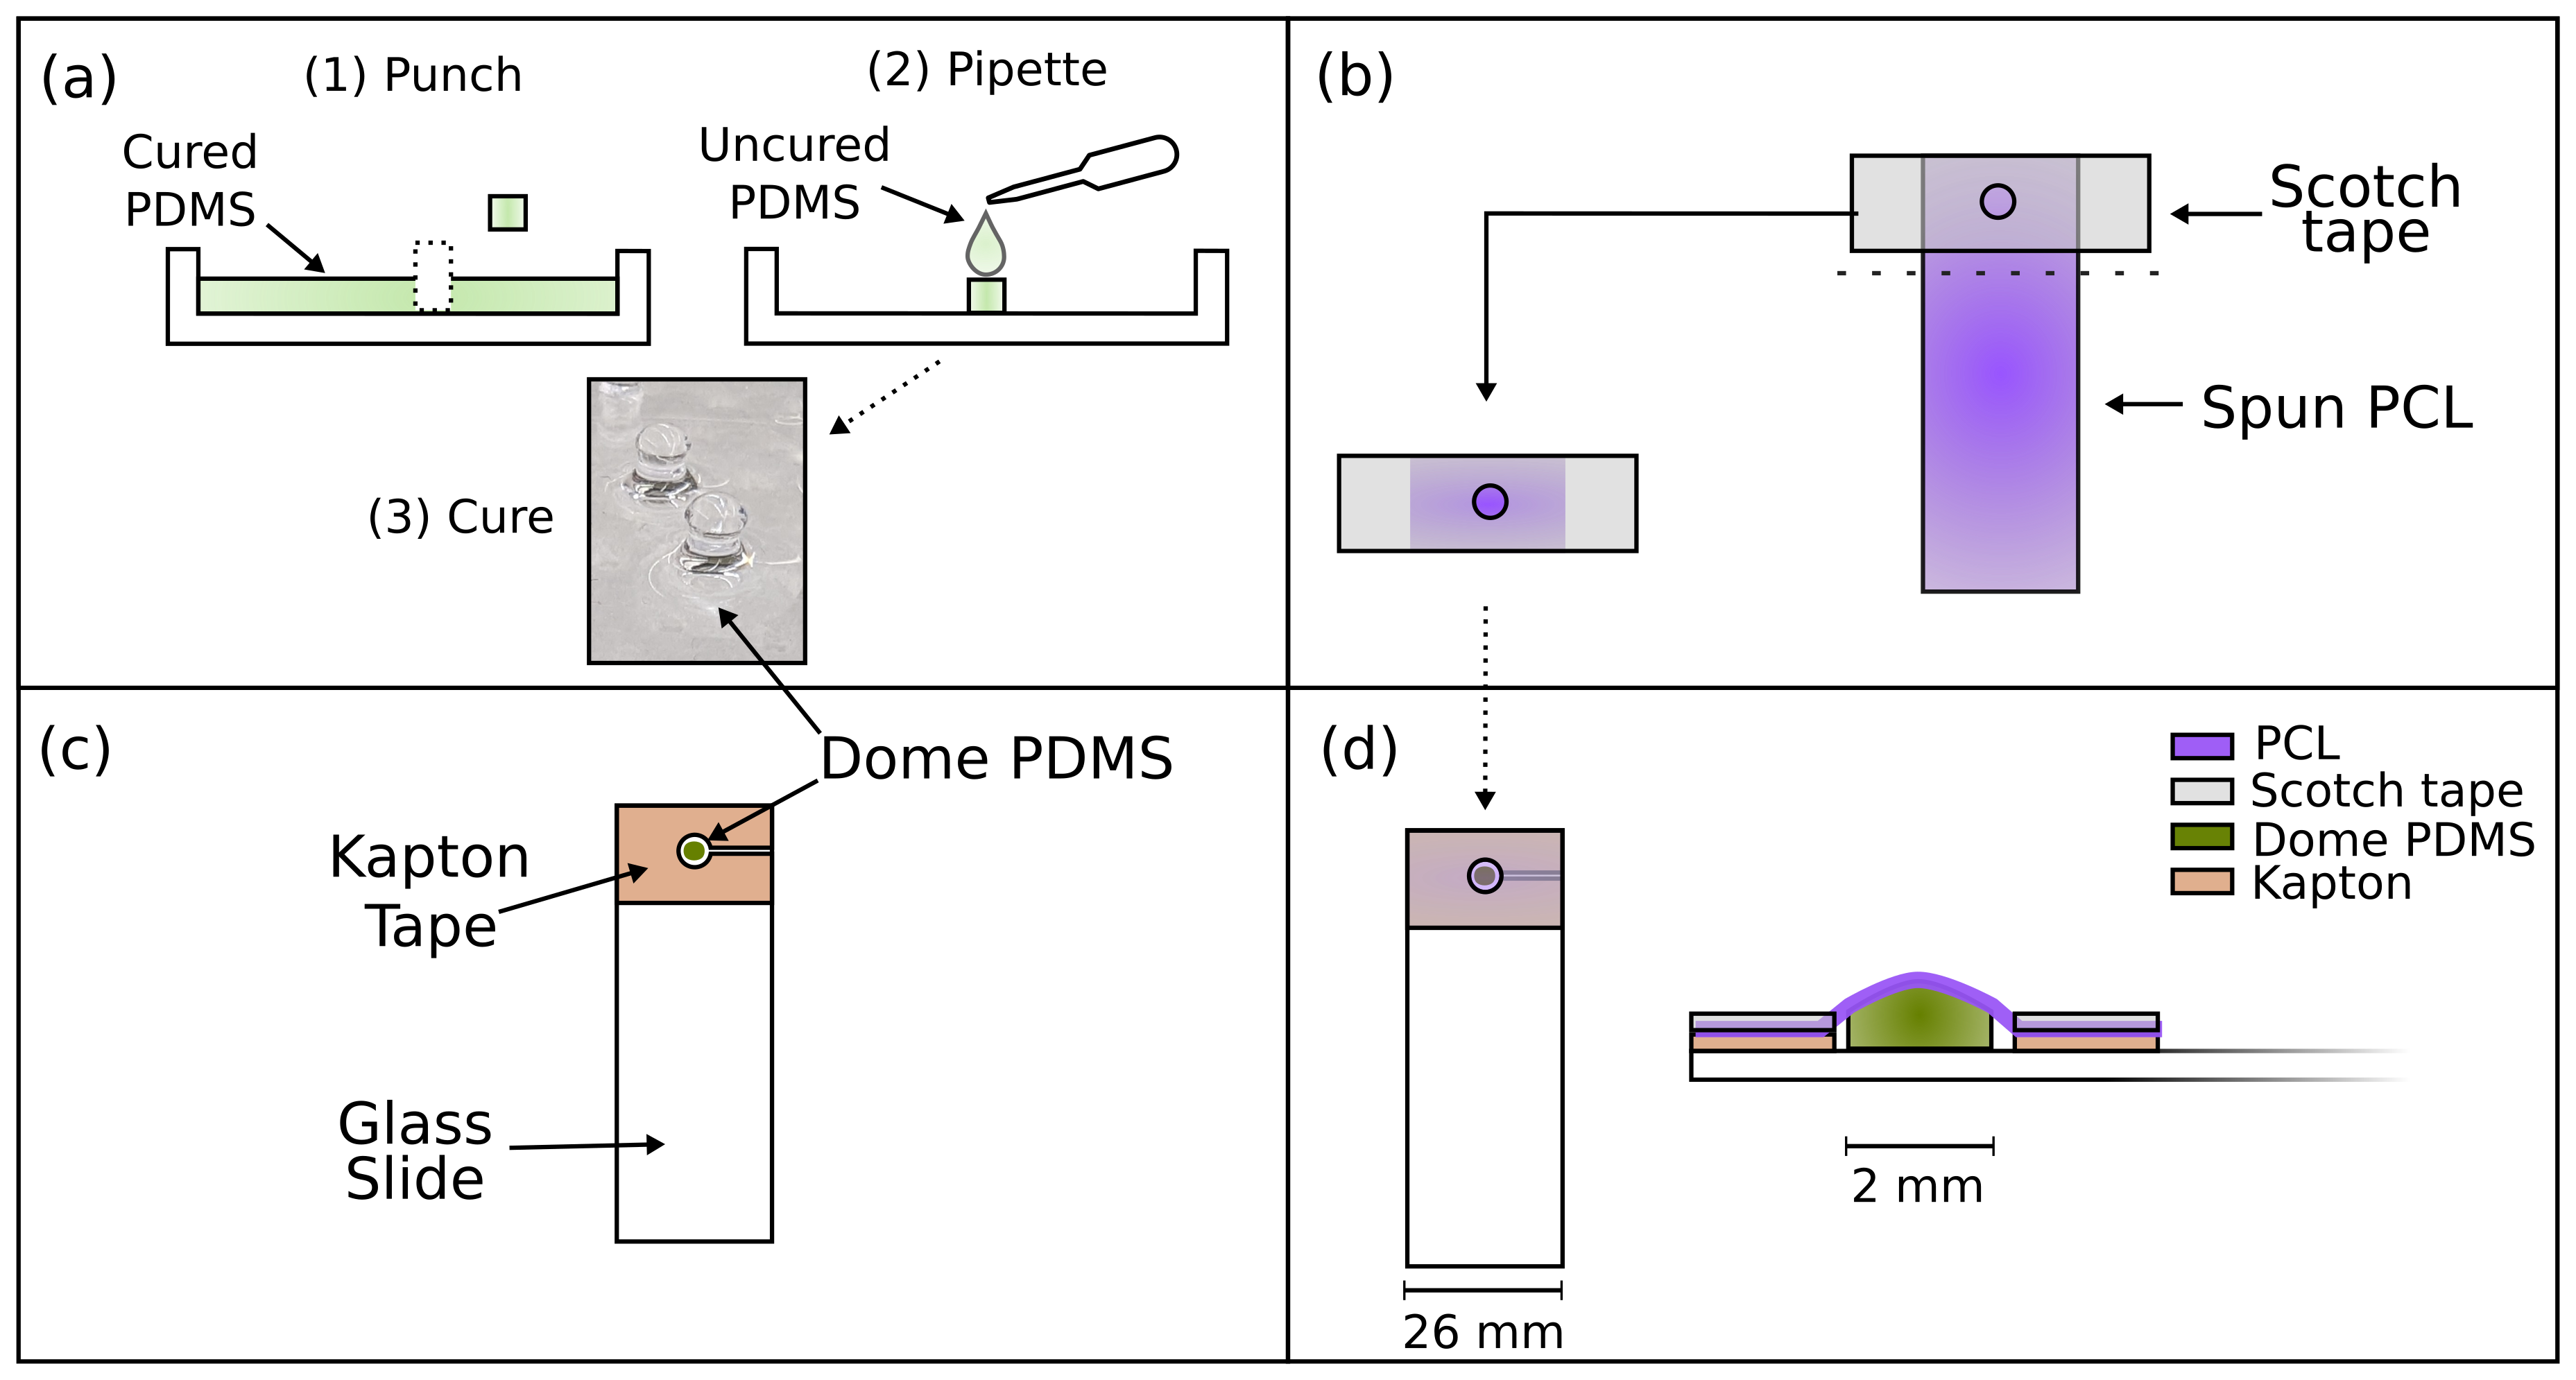
\includegraphics[width = 1\textwidth]{PCL stamp making diagram.pdf}
    \caption{(a) (1) Dome PDMS is prepared using SYLGARD™ 184 and punched out into small cylinders, then (2) uncured SYLGARD™ 184 is dripped onto the small cylinder to create a dome. The PDMS is then cured at \SI{40}{\celsius} overnight. (b) The PCL solution is spin-coated onto a clean glass slide, cured at \SI{90}{\celsius} for 1 minute, then removed using scotch tape (see Sec.\ \ref{making the PC stamp section}). (c) The slide base is prepared identically to the PC stamp, as described in Sec.\ \ref{making the PC stamp section}. (d) The PCL film is placed onto the dome PDMS, completing the PCL stamp.}
    \label{PCL stamp making diagram}
\end{figure}

\subsubsection{Using the polycaprolactone stamp}
Figure \ref{PCL cleaning process} illustrates the process of picking up unwanted flakes or tearing sections from desired flakes using a PCL stamp. First, I mount the PCL stamp onto the transfer stage (Fig.\ \ref{transfer stage image}) with the stage temperature set to \SI{30}{\celsius}. Then, I lower the PCL stamp onto a clean SiO\textsubscript{2} substrate until it contacts the surface in a circle of radius $\approx \SI{500}{\micro\meter}$. Next, I raise the stage temperature to \SI{60}{\celsius} to melt the PCL that is contacting the surface. The PCL is opaque when solid and transparent when melted. At this point, if the PCL contact area expands more than desired, I slowly raise the z-stage to stop the expansion. If the PCL is melting completely during this step, I recommend cooling the stage by \SI{5}{\celsius}. Then, I cool the stage to \SI{30}{\celsius} to solidify the PCL. To pick up or tear a flake, I lower the stamp until it is lightly contacting the substrate, then heat the stage to \SI{60}{\celsius}. Ideally, the PCL contact area will stop expanding at the edge created in the previous step. Then, I cool the stage back to \SI{30}{\celsius}. When melted, the PCL conforms well to the 2D flake, then when cooled, the flake is strongly adhered to the PCL. Lastly, once the PCL is opaque (around 2 minutes at \SI{30}{\celsius}), I raise the stamp off of the substrate, picking up any 2D flake (or part of a flake) that is inside the PCL contact area.

%TODO: Review this section and restate how you use this at the end
%PCL cleaning figure: Make figure b melt/cool cycle, and c showing PCL off surface holding its shape
%Caption the below figs.
\begin{figure}
    \includegraphics[width = 1\textwidth]{PCL cleaning process.pdf}
    \caption{(a) First, the PCL stamp is lowered until it just touches the substrate. (b) Then, the stage it heated to \SI{60}{\celsius} to melt the PCL, and (c) cooled to \SI{30}{\celsius} to solidify the PCL. This melt/cool step defines a flat edge which will stop the expansion of the polymer front. (d) The PCL stamp is placed onto the substrate, with the flakes to be picked up inside the edge. (e) Another melt/cool cycle grabs the flakes that are in contact with the PCL. (f) The stamp is raised from the substrate, grabbing all flakes (or portions of flakes) in contact with the PCL. All scale bars = \SI{100}{\micro\meter}.}
    \label{PCL cleaning process}
\end{figure}

\begin{figure}
    \includegraphics[width = 1\textwidth]{PCL before-after.pdf}
    \caption{An exfoliated graphene flake before (left) and after (right) being torn by a PCL stamp. The thick graphite areas were removed, leaving an area of uniform thickness. Scale bars = \SI{50}{\micro\meter}}
\end{figure}





\section{Contacts to 2D materials} \label{contacts to 2D materials}

\subsection{Photolithography} \label{photolithography}

In this section, I discuss methods for fabricating 2D devices on piezoelectric substrates using photolithography. One might ask: Why not use electron-beam lithography (EBL)? EBL can achieve higher lithographic resolution than photolithography and allows for custom circuit designs to match bespoke 2D heterostructures. For these reasons, EBL is an excellent choice for fabricating 2D devices on SiO\textsubscript{2}. When performing EBL on a thin ($< \SI{0.5}{\micro\meter}$) layer of insulating SiO2 on conductive Si, the charge buildup from the electron beam can readily dissipate through the thin SiO2. However, piezoelectric substrates like quartz or LiNbO\textsubscript{3} are insulating throughout, leading to charge buildup which deflects the incident electrons and distorts lithographic patterns. To dissipate the charge on insulating substrates, one can either deposit a thin charge dissipation layer on top of the EBL resist with thermal evaporation (often 10-20 nm of Al or Au), which is etched away after exposing the resist, or spin a conductive polymer on the EBL resist which is water-soluble \cite{noauthor_nanolithography_nodate}. These anti-charging layers complicate the fabrication process. Depositing a thin metal charge dissipation layer requires time-consuming thermal evaporation, and removing the metal requires a wet chemical etch. This needs to be repeated for every lithography step. Conductive polymers solve these issues but are prohibitively expensive.\footnote{The most common conductive polymer is ESpacer, which costs \$30,000 per 1 L bottle and expires after 6 months. Recently, an alternative conductive resist has been made available which is available in smaller quantities \cite{lopez_charge_2019}.}  

With the tools available to me, I can fabricate structures down to \SI{3}{\micro\meter} with photolithography. Unless a device absolutely necessitates smaller feature sizes, it is in my best interest to simplify fabrication and reduce the number of processing steps. However, the motivation for reducing processing steps goes beyond just reducing cost and complexity. In my experience, 2D device fabrication is most likely to fail during liftoff. For example, Fig.\ \ref{fig:h-BN lifted} shows a 40 nm flake of h-BN transferred onto LiNbO\textsubscript{3} (top panel) which separated from the surface during liftoff (bottom panel), taking 50 nm of metal with it. For these reasons, I use photolithography to fabricate 2D devices on piezoelectric substrates. My process involves first creating pre-patterned metal contacts which are then cleaned using AFM (refer to Section \ref{AFM cleaning main section}) prior to transferring a 2D material onto them.
\begin{figure}
    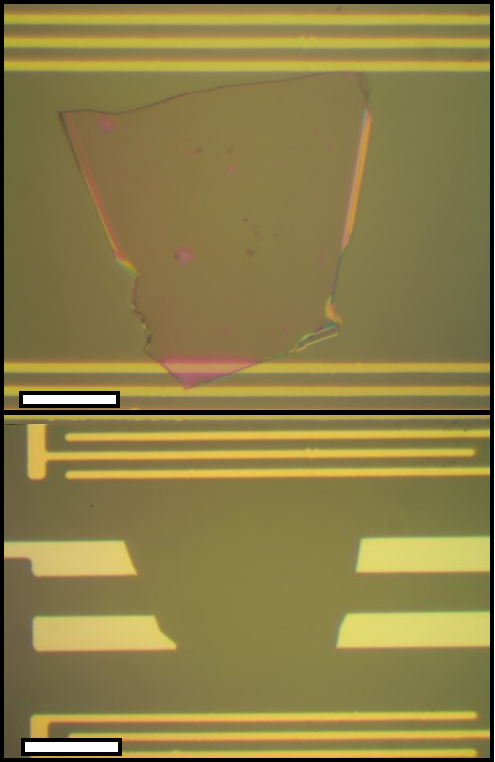
\includegraphics[width = 0.5\textwidth]{hBN lifted off.pdf}
    \caption{h-BN flake transferred onto LiNbO\textsubscript{3} before (top) and after (bottom) photolithography process to deposit metal electrodes on top of the h-BN. The h-BN lifted off with the deposited metal. Scale bar = \SI{40}{\micro\meter}.}
    \label{fig:h-BN lifted}
\end{figure}

When transferring 2D flakes onto pre-patterned metal contacts, creating a smooth surface is of paramount importance. Therefore, clean liftoff with smooth edges is necessary. For this, I use a bilayer process with a tuned undercut, with S1813 photoresist on top of LOR 3A (“liftoff resist”). The full recipe can be found in Appx.\ \ref{photolithography recipe}. Figure \ref{fig:Liftoff AFM} shows a comparison between single-layer and bilayer liftoff processes in which I attempted to lift off $\approx \SI{25}{\nano\meter}$ of Cr deposited on SiO\textsubscript{2} using electron-beam evaporation. In the single-layer process, metal which coated the resist walls did not lift off with the resist, creating wings that are much taller than the metal thickness. In a bilayer process, the bottom layer of resist develops faster than the top layer, creating an undercut profile that breaks the connection between the metal on the resist walls and the desired pattern. It’s clear that a bilayer process is necessary for pre-patterned 2D material contacts. 




\begin{figure}
    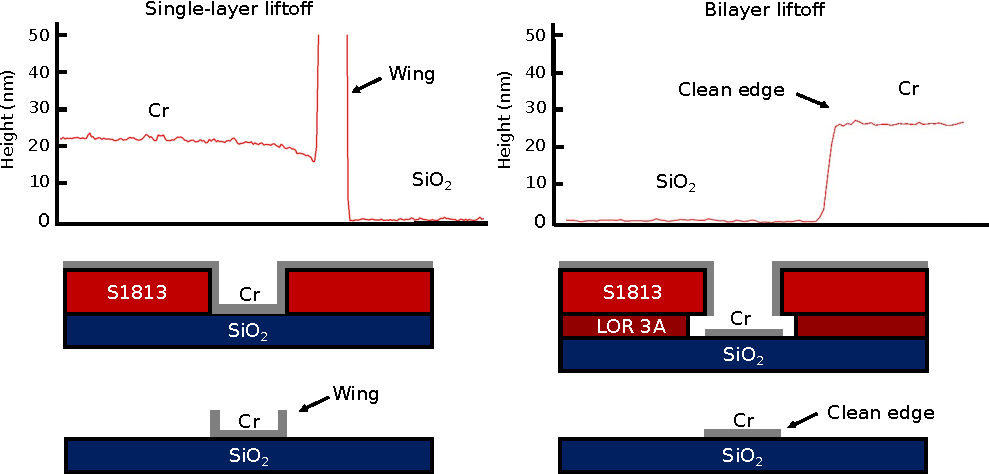
\includegraphics[width = 1\textwidth]{liftoff AFM traces comparison.pdf}
    \caption{AFM trace (top) and schematic (bottom) for single-layer (left) and bilayer (right) liftoff processes of Cr on SiO\textsubscript{2}.}
    \label{fig:Liftoff AFM}
\end{figure}

The development rate of the LOR can be tuned by varying the bake temperature. A higher temperature bake results in a slower undercut rate, allowing us to optimize the undercut. If the undercut is too large, the top layer of resist will collapse. If the undercut is too small, the metal will not lift off cleanly. I first determined the optimal development time for S1813 as 100 seconds using the interdigitated finger pattern shown in Fig.\ \ref{fig:h-BN lifted}. Then, I varied the LOR bake time from 170 C to 190 C and attempted liftoff of 3/20 nm Cr/Au. I found that 180 C was the lowest bake temperature at which liftoff was clean. Figure \ref{AECP Figure 2}.4 shows a cross-sectional SEM image, in which I confirmed that a 180 C bake and 100 s development creates $\approx \SI{3}{\micro\meter}$ undercut.

The drawback of transferring 2D materials onto pre-patterned contacts is that the contacts need to be cleaned to minimize contamination of the 2D material. In the next section, I detail a method for cleaning metal contacts with contact-mode AFM.


\begin{figure}
    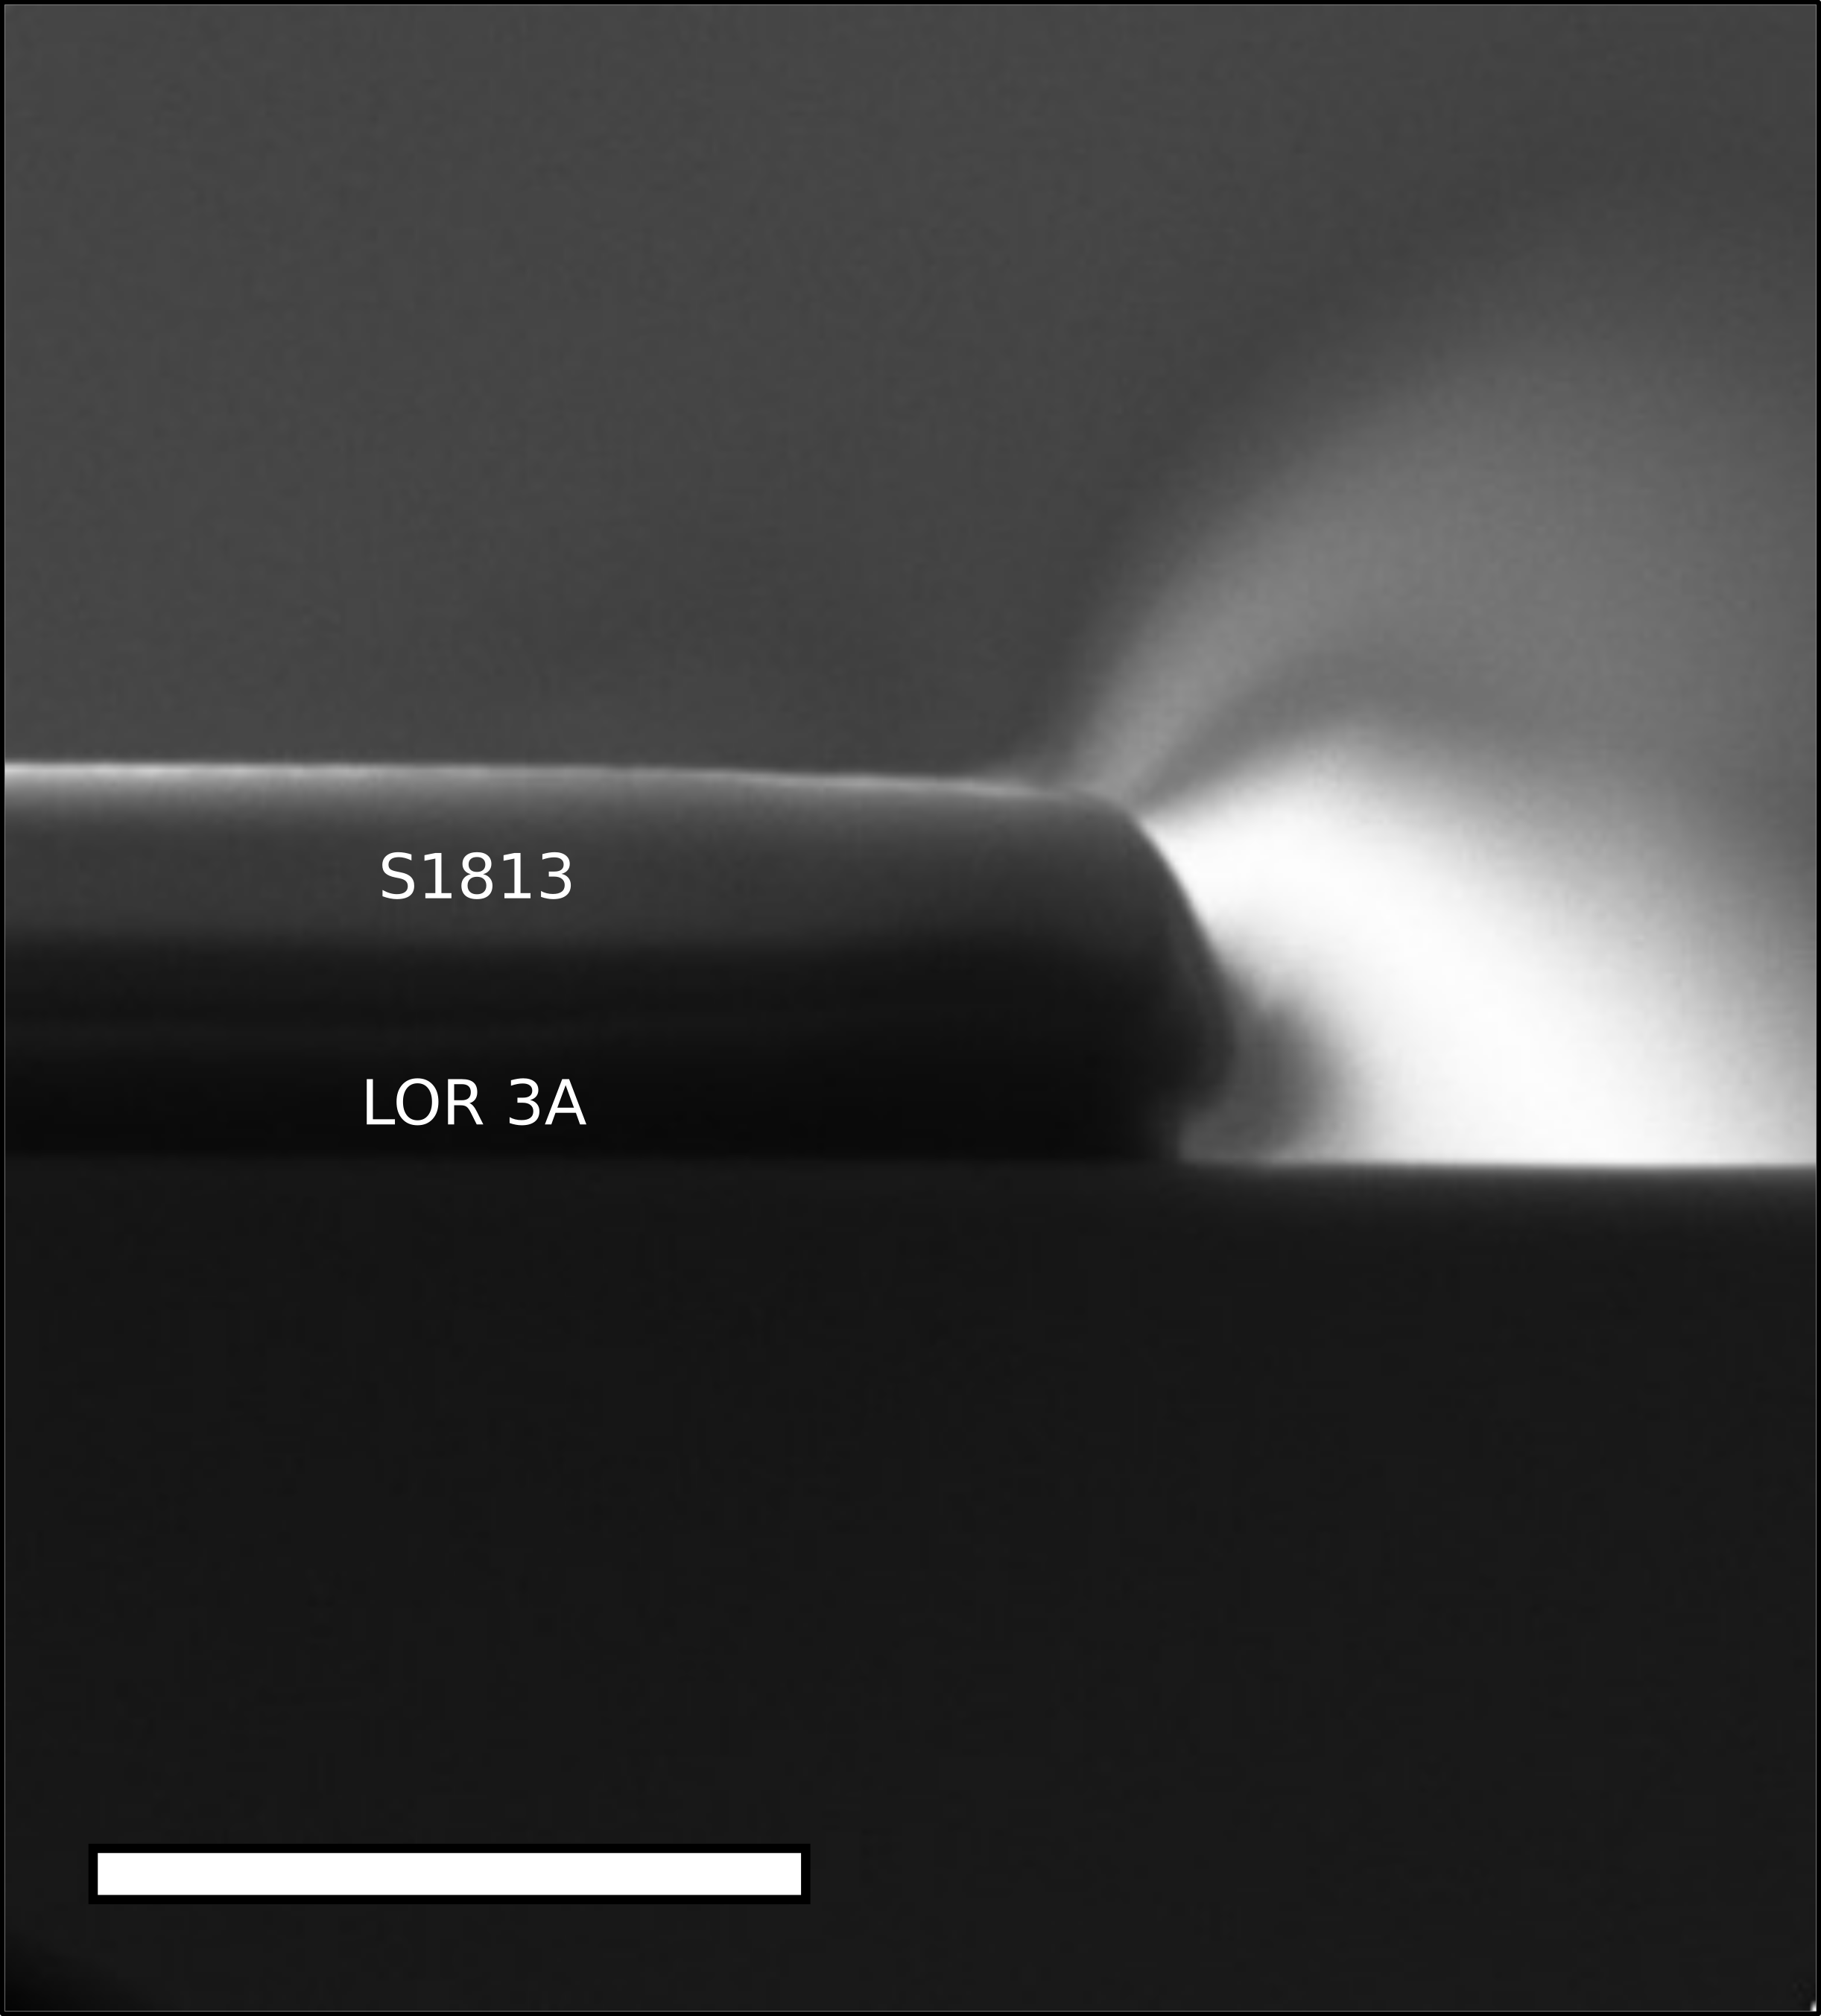
\includegraphics[width = 0.6\textwidth]{LOR cross section_.png}
    \caption{Cross-sectional SEM image showing bilayer resist process with undercut length $\approx \SI{0.4}{\micro\meter}$. Scale bar = \SI{3}{\micro\meter}.}
    \label{fig:cross-section SEM}
\end{figure}

\subsection{Cleaning electrodes with contact mode atomic force microscopy} \label{AFM cleaning main section}

As-deposited metal contacts will inevitably retain residues from the resist and solvents utilized during the photolithography process. Previously, contact-mode AFM has been used to remove contaminants from beneath 2D materials \cite{goossens_mechanical_2012,chen_tip-based_2021}. However, to create the devices described in Ch.\ \ref{AE charge pumping paper}, I use contact-mode AFM to clean pre-patterned metal electrodes prior to transferring graphene onto them. I learned this technique from the Yankowitz group at the University of Washington.

For this process, I use Tap150AL AFM probes (Budget Sensors) and an MFP-3D AFM. I first measure the exact spring constant of the AFM tip by taking a force curve. For the full force curve process and a sample force curve, see Appendix \ref{force curve appendix}. Then, I scan the AFM across the electrodes at a force of \SI{150}{N} and a speed of \SI{150}{\micro\meter/\second}. The AFM scan size is \SI{35}{\micro\meter} in the scan direction, and the Tap150AL tip has a minimum diameter of \SI{10}{\nano\meter}. I chose 3584 lines for the scan (\SI{9.76}{\nano\meter/line}) to ensure that each line slightly overlaps the previous line. Figure \ref{AFM cleaning points} shows Pd electrodes after two AFM cleaning runs: One scan perpendicular to the electrodes, then one scan parallel to the electrodes. A significant amount of residue has been displaced by the AFM tip, and is visible at the edge of the clean area. For the devices described in Ch.\ \ref{AE charge pumping paper}, I use this process to clean pre-patterned Pd electrodes before transferring graphene onto them.

\begin{figure}
    \includegraphics[width = 0.6\textwidth]{AFM cleaning 1.pdf}
    \caption{An optical microscope image of Pd electrodes on LiNbO\textsubscript{3} after two perpendicular AFM cleaning scans at a force of \SI{150}{N} and a speed of \SI{150}{\micro\meter/\second}. Scale bar = \SI{40}{\micro\meter}.}
    \label{AFM cleaning points}
\end{figure}


\section{Fabrication and measurement of interdigitated transducers} \label{IDT methods}

Before using an interdigitated transducer to pump charge in graphene (Ch.\ \ref{AE charge pumping paper}), I need to verify its performance. In Sec.\ \ref{SAW device design}, I outline the expected frequency response and impedance of an IDT based on its geometry. In this section, I discuss my methods for measuring the frequency response and impedance of IDTs to verify their performance, and compare my measurements to the theory presented in Sec.\ \ref{SAW device design}.

Figure \ref{SAW device optical image with measurements} shows an optical microscope image of a pair of IDTs that I fabricated on black LiNbO\textsubscript{3} using photolithography (see Appx.\ \ref{photolithography recipe} for recipe) and metallization of $5/\SI{25}{\nano\meter}$ Al using electron-beam evaporation. Black LiNbO\textsubscript{3} has identical piezoelectric properties to ordinary LiNbO\textsubscript{3}, but is free of the pyroelectric effect, so it can tolerate faster thermal ramps without cracking.



\begin{figure}
    \includegraphics[width = 1\textwidth]{SAW device optical image 1.pdf}
    \caption{Optical microscope image of a pair of IDTs on black LiNbO\textsubscript{3} with parameters $N_p = 20$, $W = \SI{230}{\micro\meter}$, and $\lambda = \SI{20}{\micro\meter}$. Scale bar = $\SI{100}{\micro\meter}$.}
    \label{SAW device optical image with measurements}
\end{figure}
These IDTs have $N_p = 20$ finger pairs and aperture width $W = \SI{230}{\micro\meter}$. Their wavelength is $\lambda = \SI{20}{\micro\meter}$ and the SAW velocity on LiNbO\textsubscript{3} is \SI{3488}{\meter/\second}, giving a center frequency of $f_0 = \SI{174.4}{\mega\hertz}$. Using Eq.\ \ref{IDT admittance}, the impedance of this IDT should be $Z_{IDT} \approx \SI{170}{\ohm}$. 

To benchmark the performance of the IDT pair, I use an Agilent E5071C-280 vector network analyzer to measure their S-parameters and impedance. Figure \ref{S-parameters} (a) shows the definition of the four S-parameters for a two-port network. $S_{11}$ and $S_{22}$ are the ratios of reflected RF power to input RF power for IDT 1 and IDT 2 respectively. $S_{21}$ is the ratio of received RF power at IDT 2 to input RF power at IDT 1, and $S_{12}$ is the ratio of received RF power at IDT 1 to input RF power at IDT 2. Figure \ref{S-parameters} (b) shows S11 and S22, and Fig.\ \ref{S-parameters} (b) shows S21 and S12 for IDT 1 and IDT 2 (Fig.\ \ref{SAW device optical image with measurements}).


\begin{figure}
    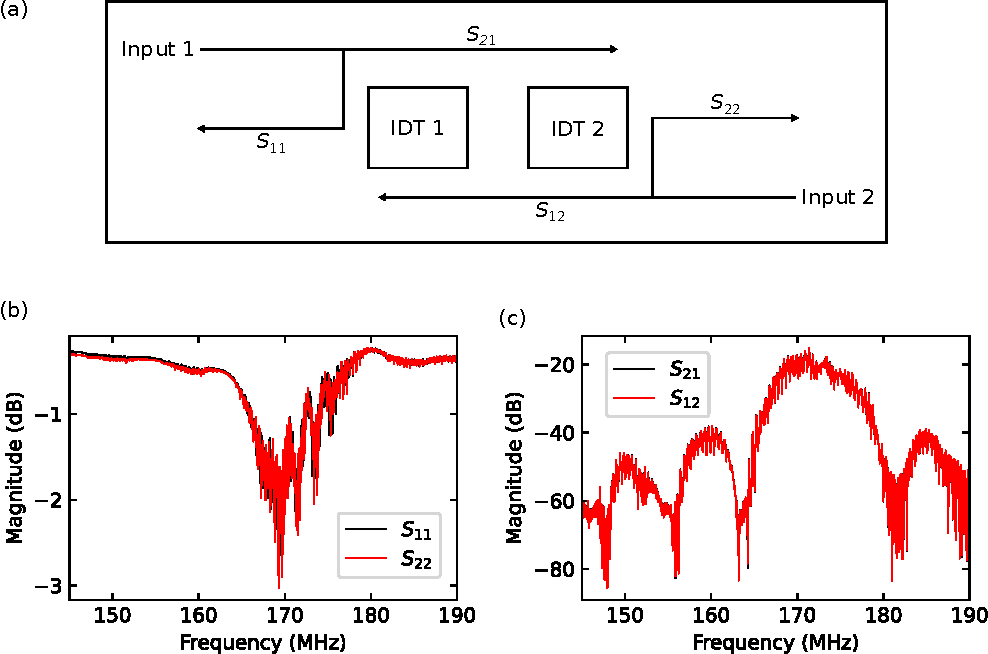
\includegraphics[width = 1\textwidth]{S-parameters.pdf}
    \caption{(a) Definition of S-parameters for a two-port network. (b) $S_{11}$ and $S_{22}$ for IDT 1 and IDT 2 shown in Fig.\ \ref{SAW device optical image with measurements}. A drop in $S_{11}$ ($S_{22}$) is seen near the center frequency $f_0 = v/\lambda = \SI{174.4}{\mega\hertz}$, corresponding to the increase in $S_{21}$ ($S_{12}$).}
    \label{S-parameters}
\end{figure}
The S-parameter data shown in Fig.\ \ref{S-parameters} (b) and (c) are in good agreement with the model discussed in Sec.\ \ref{SAW device design}. First, there is a drop in reflected power at $f \approx \SI{170}{\mega\hertz}$, close to $f_0$, (Fig.\ \ref{S-parameters} (b)), which corresponds to the increase in transmitted power (Fig.\ \ref{S-parameters} (c)). It is normal for the IDT center frequency to be slightly lower than expected due to mass-loading effects, depending on the density and thickness of the metal used. As $f_0$ increases, using low-density, thin metal becomes more important to minimize the mass-loading-driven shift in $f_0$ \cite{chen_ultrahigh-frequency_2020}. This effect is less pronounced for IDTs in the MHz range. Away from $f_0$, secondary resonance peaks of decreasing magnitude can be seen in the $S_{21}$ and $S_{12}$ data. This is in agreement with the frequency response predicted by Eq.\ \ref{Response of IDT}. Lastly, the frequency response curves of the two IDTs are nearly indistinguishable, showing that the geometry of each IDT is identical. 

Figure \ref{Z11 plot} shows the measured real part of the admittance ($\mathrm{Re}(Y)$) of IDT 1 in comparison to the model given by Eq.\ \ref{IDT admittance}. The measured admittance at $f_0$ is $\SI{6.5}{\milli\siemens} = (\SI{154}{\ohm})^{-1}$, while the model predicts an admittance of $\SI{5.9}{\milli\siemens} = (\SI{170}{\ohm})^{-1}$ (a difference of $10\%$). Also, the width of the peak in $Re(Y)$ is wider than predicted by the model. This discrepancy is most likely because the model given by Eq.\ \ref{IDT admittance} does not consider reflections from each IDT finger. This IDT has $N_p = 20$, and each finger reflects around 0.1 \textemdash 2 \% of the IDT signal \cite[p.140]{lane_integrating_2021}.

From Eq.\ \ref{reflection coefficient} and a purely real input impedance of $\SI{50}{\ohm}$, $\approx 70\%$, of the input RF power is reflected back from the IDT. This could be improved; however, this IDT has similar $S_{21}/S_{12}$ performance to prior IDTs used in charge pumping experiments \cite{buitelaar_charge_2006}, so I deemed the performance of these IDTs good enough to proceed. I use this IDT design for the devices described in Ch.\ \ref{AE charge pumping paper}.

\begin{figure}
    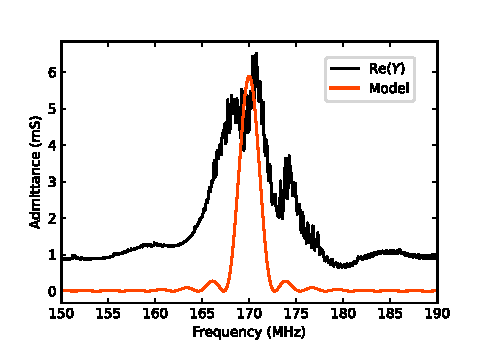
\includegraphics[width = 0.75\textwidth]{Z11_plot_.pdf}
    \caption{Measured real part of the admittance $Y_{11}$ of IDT 1 compared to the model given by Eq.\ \ref{IDT admittance}. The center frequency of the model has been shifted to match the measured center frequency.}
    \label{Z11 plot}
\end{figure}

\chapter{Charge pumping in h-BN encapsulated graphene driven by surface acoustic waves}\label{AE charge pumping paper}

\clearpage

\mbox{}
\vspace{3cm}
\begin{center}
    {\large CHARGE PUMPING IN h-BN-ENCAPSULATED GRAPHENE DRIVEN BY SURFACE ACOUSTIC WAVES}
    \vspace{4cm}

    \underline{Dublin M. Nichols}, Jameson G. Berg, Takashi Taniguchi, Kenji Watanabe, Pallavi Dhagat, Vikram V. Deshpande, Albrecht Jander, and Ethan D. Minot
    \vspace{3cm}

    \textit{Journal of Applied Physics} \textbf{136}, 024302 (2024); doi: 10.1063/5.0220123
\end{center}

\pagebreak
\begin{figure}
    \includegraphics[width = 0.65\textwidth]{Highlight figure final v2.jpg}
\end{figure}

\section*{Abstract}
Surface acoustic waves (SAWs) on piezoelectric insulators can generate dynamic periodic potentials inside one-dimensional and two-dimensional materials. These periodic potentials have been utilized or proposed for various applications, including acoustoelectric charge pumping. In this study, we investigate acoustoelectric charge pumping in graphene with very low electrostatic disorder. By employing a graphite top gate on boron-nitride-encapsulated graphene, we adjust the graphene carrier concentration over a broad range, enabling us to examine the acoustoelectric signal in both mixed-carrier and single-carrier regimes. We discuss the benefits of h-BN-encapsulated graphene for charge pumping applications and introduce a model that describes the acoustoelectric signal across all carrier concentrations, including at the charge neutrality point. This quantitative model will support future SAW-enabled explorations of phenomena in low-dimensional materials and guide the design of novel SAW sensors.
\clearpage

%TODO: Insert equations here
\section{Introduction} 

Surface acoustic waves (SAWs) offer the possibility to create dynamic superlattices in 1D and 2D materials. When a SAW propagates across a strong piezoelectric insulator, the extension and compression of the insulator generates a periodic potential. SAWs can be generated with wavelengths ranging from tens of microns to tens of nanometers. In the burgeoning field of van der Waals heterostructures made from 2D materials, SAWs have emerged as a new way to interact with charge carriers. For example, previous work has demonstrated the transport of indirect excitons in 2D semiconductor heterostructures \cite{peng_long-range_2022}, and contactless probing of quantum oscillations in graphene \cite{fang_quantum_2023}.

Interest in applying SAWs to 1D and 2D materials is inspired by previous experiments on GaAs/AlGaAs quantum wells, and by a number of outstanding theoretical proposals. For example, photogenerated electron-hole pairs in GaAs were separated by a SAW potential, and then released to generate photons \cite{rocke_acoustically_1997}. SAWs were utilized in conjunction with Coulomb blockade to sequentially transport single electrons through a quantum point contact \cite{talyanskii_single-electron_1997}. New insights into the quantum Hall effect and fractional quantum Hall effect in GaAs/AlGaAs quantum wells were obtained by utilizing commensurability effects with a SAW superlattice \cite{willett_experimental_1993,kukushkin_collective_2011}. Turning to examples of theoretical proposals, Barnes et al. formulated a scheme for quantum computing using single electrons trapped in SAW potential minima (“flying qubits”) \cite{barnes_quantum_2000,gumbs_quantum_2004,giavaras_quantum_2006}. Andreev recently proposed that a SAW applied to charge-neutral graphene can efficiently pump heat (approaching the Carnot limit) \cite{andreev_electronic_2022}. Talyanskii et al. proposed a scheme in which a carbon nanotube can realize a topologically protected electron pump, defining a quantum standard for the current \cite{talyanskii_quantized_2001}.

It is challenging to cleanly integrate SAWs with 1D and 2D electronic systems because many insulating surfaces (including piezoelectric insulators) introduce significant electrostatic disorder to the electronic system. This disorder disrupts the intrinsic properties of the low-dimensional material. To overcome this issue, Dean et al. introduced a method of encapsulating low-dimensional materials with hexagonal boron nitride (h-BN), an ultraclean 2D insulator \cite{dean_boron_2010}. Boron-nitride-encapsulated graphene has been utilized for many applications; for example, demonstrating the highest-performing Hall-effect sensor \cite{schaefer_magnetic_2020}. However, there are no previous studies of acoustoelectric charge pumping in h-BN-encapsulated graphene. In this work, we address the need for a detailed, quantitative analysis of the interaction between SAWs and graphene when electrostatic disorder is significantly reduced. Moreover, by using h-BN encapsulation, we expect improvements such as larger pumping currents and increased sensitivity of pumping current with respect to carrier concentration, which may aid future technologies. 

Previous authors have demonstrated acoustoelectric charge pumping in lower-quality graphene samples (see review by Hernández-Mínguez et al. \cite{hernandez-minguez_interaction_2018}), but device quality (and sometimes non-tunable carrier concentration) has hindered quantitative comparison with theory. In our device design, the electric field from the SAW couples to the graphene from below, while a graphite top gate enables us to tune the carrier concentration in graphene over a wide range. We demonstrate that the SAW can drive extremely high 2D current density in h-BN-encapsulated graphene when the system is tuned close to the charge neutrality point (CNP). At the largest SAW powers, we see signs of nonlinear effects, suggesting that the SAW causes a perturbation in carrier density that is comparable to the equilibrium carrier density.  We present a theoretical model to describe the acoustoelectric current/voltage as a function of charge carrier concentration. In contrast to previous work, we extend the classical relaxation model to account for the coexistence of electrons and holes near the CNP. Our mixed-carrier model describes the observed acoustoelectric transport signals at all carrier concentrations, including the CNP.

\begin{figure}
    \includegraphics{Figure 1 overview.png}
    \caption{Overview of the experiment. (a) Optical microscope image of the interdigitated transducer (IDT) and an h-BN-encapsulated graphene device (device 1). The three electrodes are labeled source, drain, and gate. (b) The acoustoelectric voltage ($V_{\mathrm{ae}}$), is measured across the source (S), drain (D) electrodes. The gate electrode (G) is used to tune carrier concentration. The total resistance of the graphene device includes the left and right contact resistance ($R_{\mathrm{C1}}$  and $R_{\mathrm{C2}}$) and the graphene channel resistance ($R_{\mathrm{ch}}$).}
    \label{AECP Figure 1}
\end{figure}
\section{Background}

When the traveling electric field generated by a surface acoustic wave (SAW) passes over a conductive 2D material, charge carriers move in response to the electric field. This interaction transfers energy and momentum to the carriers and attenuates the SAW. The classical relaxation model predicts the attenuation of the SAW will be described by an attenuation constant \cite{wixforth_surface_1989}

\begin{equation}
    \Gamma = K^2\frac{\pi}{\lambda}\left[\frac{\sigma/\sigma_c}{1+ (\sigma/\sigma_c)^2}\right]
    \label{AECP Equation 1}
\end{equation}
where $K^2$ is the piezoelectric coupling constant, $\lambda$ is the wavelength of the SAW, $\sigma$ is the conductivity of the 2D material, and $\sigma_c = v_{\mathrm{SAW}}(\epsilon_1 + \epsilon_2)$  is a characteristic conductivity defined by the properties of the substrate, where $\epsilon_1$ and $\epsilon_2$ are the dielectric permittivities above and below the 2D material and $v_{\mathrm{SAW}}$ is the SAW velocity in the piezoelectric substrate. For a 2D material on LiNbO\textsubscript{3},$K^2= 0.05$ and $\sigma_c \approx (\SI{1}{\mega\ohm})^{-1}$  \cite{wixforth_surface_1989,rotter_giant_1998}.

If the 2D material is wired in a short-circuit configuration, the classical relaxation model predicts that the SAW will drive a net flow of charge through the 2D material \cite{rotter_giant_1998}. The predicted short-circuit acoustoelectric current density is given by

\begin{equation}
    j_{\mathrm{ae}} = \pm \frac{\mu I}{v_{\mathrm{SAW}}}\Gamma
    \label{AECP Equation 2}
\end{equation}
where the sign is determined by the sign of the carriers (negative for electrons, positive for holes), $\mu$ is the carrier mobility, and $I \propto P_{\mathrm{RF}}/W$ is the SAW intensity at the 2D material, where $P_{\mathrm{RF}}$ is the power applied to the interdigitated transducer (IDT) and $W$ is the aperture width of the IDT used to drive the SAW. In experiments, there is a decrease in power between the RF generator and the SAW (insertion loss) which can be described by a proportionality constant. Equations \ref{AECP Equation 1} and \ref{AECP Equation 2} assume a single carrier type (either electrons or holes) and predict that $j_{\mathrm{ae}}$ is maximized when $\sigma = \sigma_c$. However, in graphene, the model must be adjusted to describe a system in the mixed-carrier regime.


\section{Experiment design} \label{charge pumping paper experiment design}
Figure 1 (b) illustrates our experimental measurement scheme. To detect the acoustoelectric voltage, $V_{\mathrm{ae}}$, we probe the open-circuit voltage across the graphene channel. There is an effective force on charge carriers from the SAW which pushes charge carriers towards one side of the channel.  Since there is no net current in the open-circuit configuration, an acoustoelectric voltage develops to balance the force from the SAW. The relationship between expected $V_{\mathrm{ae}}$ (open-circuit voltage) and $j_{\mathrm{ae}}w$ (short-circuit current) is $j_{\mathrm{ae}}w = V_{\mathrm{ae}}$/$R_{\mathrm{ch}}$, where $R_{\mathrm{ch}}$ is the resistance of the graphene channel and w is the width of the graphene channel measured perpendicular to the SAW propagation direction. We use $V_{\mathrm{ae}}$ for our analysis because a true measurement of short-circuit current requires zero-resistance contacts to the graphene, and a zero-impedance current amplifier. Previous attempts to quantify $j_{\mathrm{ae}}$ in graphene using the short-circuit current method likely suffered from the complication of large series resistance \cite{bandhu_macroscopic_2013,bandhu_controlling_2016,okuda_acoustic_2016,tang_ultra-low_2017,okuda_graphene_2018}. 

An IDT that emits a SAW with wavelength $\lambda =  \SI{20}{\micro\meter}$ from an aperture $W = \SI{230}{\micro\meter}$ was fabricated on Y-cut black LiNbO\textsubscript{3} (University Wafer) using photolithography and metallization of 5/25 nm Cr/Au. Black LiNbO\textsubscript{3} was chosen because the material can tolerate faster thermal ramps than transparent LiNbO\textsubscript{3}  \cite{fang_quantum_2023,lane_flip-chip_2018}. Graphene devices were constructed next to the IDT as follows: First, we fabricated source/drain contacts (2.5/15 nm Cr/Pd) with channel spacing $l = \SI{20}{\micro\meter}$ (equal to $\lambda$) which sit \SI{200}{\micro\meter} from the IDT. These contacts were cleaned using an atomic force microscope (AFM) in contact mode with a force of \SI{100}{\nano\newton} \cite{goossens_mechanical_2012}. Then, we exfoliated the few-layer graphene and hexagonal boron nitride (h-BN) crystal flakes onto blank silicon wafers (\SI{300}{\nano\meter} oxide). We found large, uniform-thickness flakes using optical microscopy, and measured flake thicknesses using AFM. We used a strongly adhesive polycaprolactone (PCL) stamp to remove unwanted graphene flakes (reducing the likelihood that unwanted graphene flakes would short the IDT), and to tear the channel graphene flakes into rectangular pieces of a single thickness \cite{son_strongly_2020}. We then used a PC/PDMS (poly(bisphenol A carbonate)/polydimethylsiloxane) stamp and the standard dry transfer technique \cite{wang_one-dimensional_2013} to create the van der Waals heterostructure and to place the stack on the prefabricated source/drain contacts. Metal contact to the graphite top gate was made by a final photolithography and metallization step (2.5/45 nm Cr/Au).

Our aim was to create devices with different levels of electrostatic disorder so we could study the effect of disorder on the acoustoelectric signal. The graphene channel of device 1 is fully encapsulated in h-BN to minimize electrostatic disorder (see inset of Fig.\ \ref{AECP Figure 2} (c)) \cite{dean_boron_2010}. The graphene channel of device 2 is half-encapsulated such that the graphene lies directly on the LiNbO\textsubscript{3} substrate (see inset of Fig.\ \ref{AECP Figure 2} (d)). The LiNbO\textsubscript{3} substrate induces electrostatic disorder in the graphene channel. For device 1, we selected two h-BN flakes, one graphene flake for the channel, and one graphite flake for the gate. The bottom h-BN flake was selected to cover the gap between the source and drain contacts. The graphene flake was selected to extend beyond the bottom h-BN flake and make electrical contact to the source and drain, as shown in Fig.\ \ref{AECP Figure 2} (c). The gate insulator of device 1 is \SI{29}{\nano\meter} h-BN, giving gate capacitance $C_g = \SI{0.11}{\micro\farad/\centi\meter^2}$. The gate insulator of device 2 is \SI{13}{\nano\meter} h-BN, giving $C_g = \SI{0.11}{\micro\farad/\centi\meter^2}$. 

\section{Results} \label{AE charge pumping results}

Figure \ref{AECP Figure 2} (a) and (b) show $V_{\mathrm{ae}}$ as a function of the spatially averaged carrier concentration in device 1 (fully encapsulated) and device 2. The transport curves have been shifted along the $V_g$-axis to align the CNP with $V_g=0$. The open-circuit voltage was measured while driving the IDT at its resonance of \SI{170}{\mega\hertz} using an Agilent N5183A analog signal generator, using a Stanford SR560 voltage preamplifier, filtered with the internal \SI{30}{\hertz} low-pass filter of the SR560. We verified that the frequency dependence of $V_{\mathrm{ae}}$ closely follows the spectrally resolved measurement of RF power absorbed by the interdigitated transducer (see Supplementary Material). Figure \ref{AECP Figure 2} (a) and (b) show other features that are expected for acoustoelectric transport. At the CNP, the sign of $V_{\mathrm{ae}}$ reverses (indicating that the SAW pushes electrons and holes in the same direction). The magnitude of $V_{\mathrm{ae}}$ changes non-monotonically with increasing carrier density. At large carrier concentrations, $V_{\mathrm{ae}}$ decays asymptotically toward zero, consistent with Eqs. \ref{AECP Equation 1} and \ref{AECP Equation 2}. 

\begin{figure}
    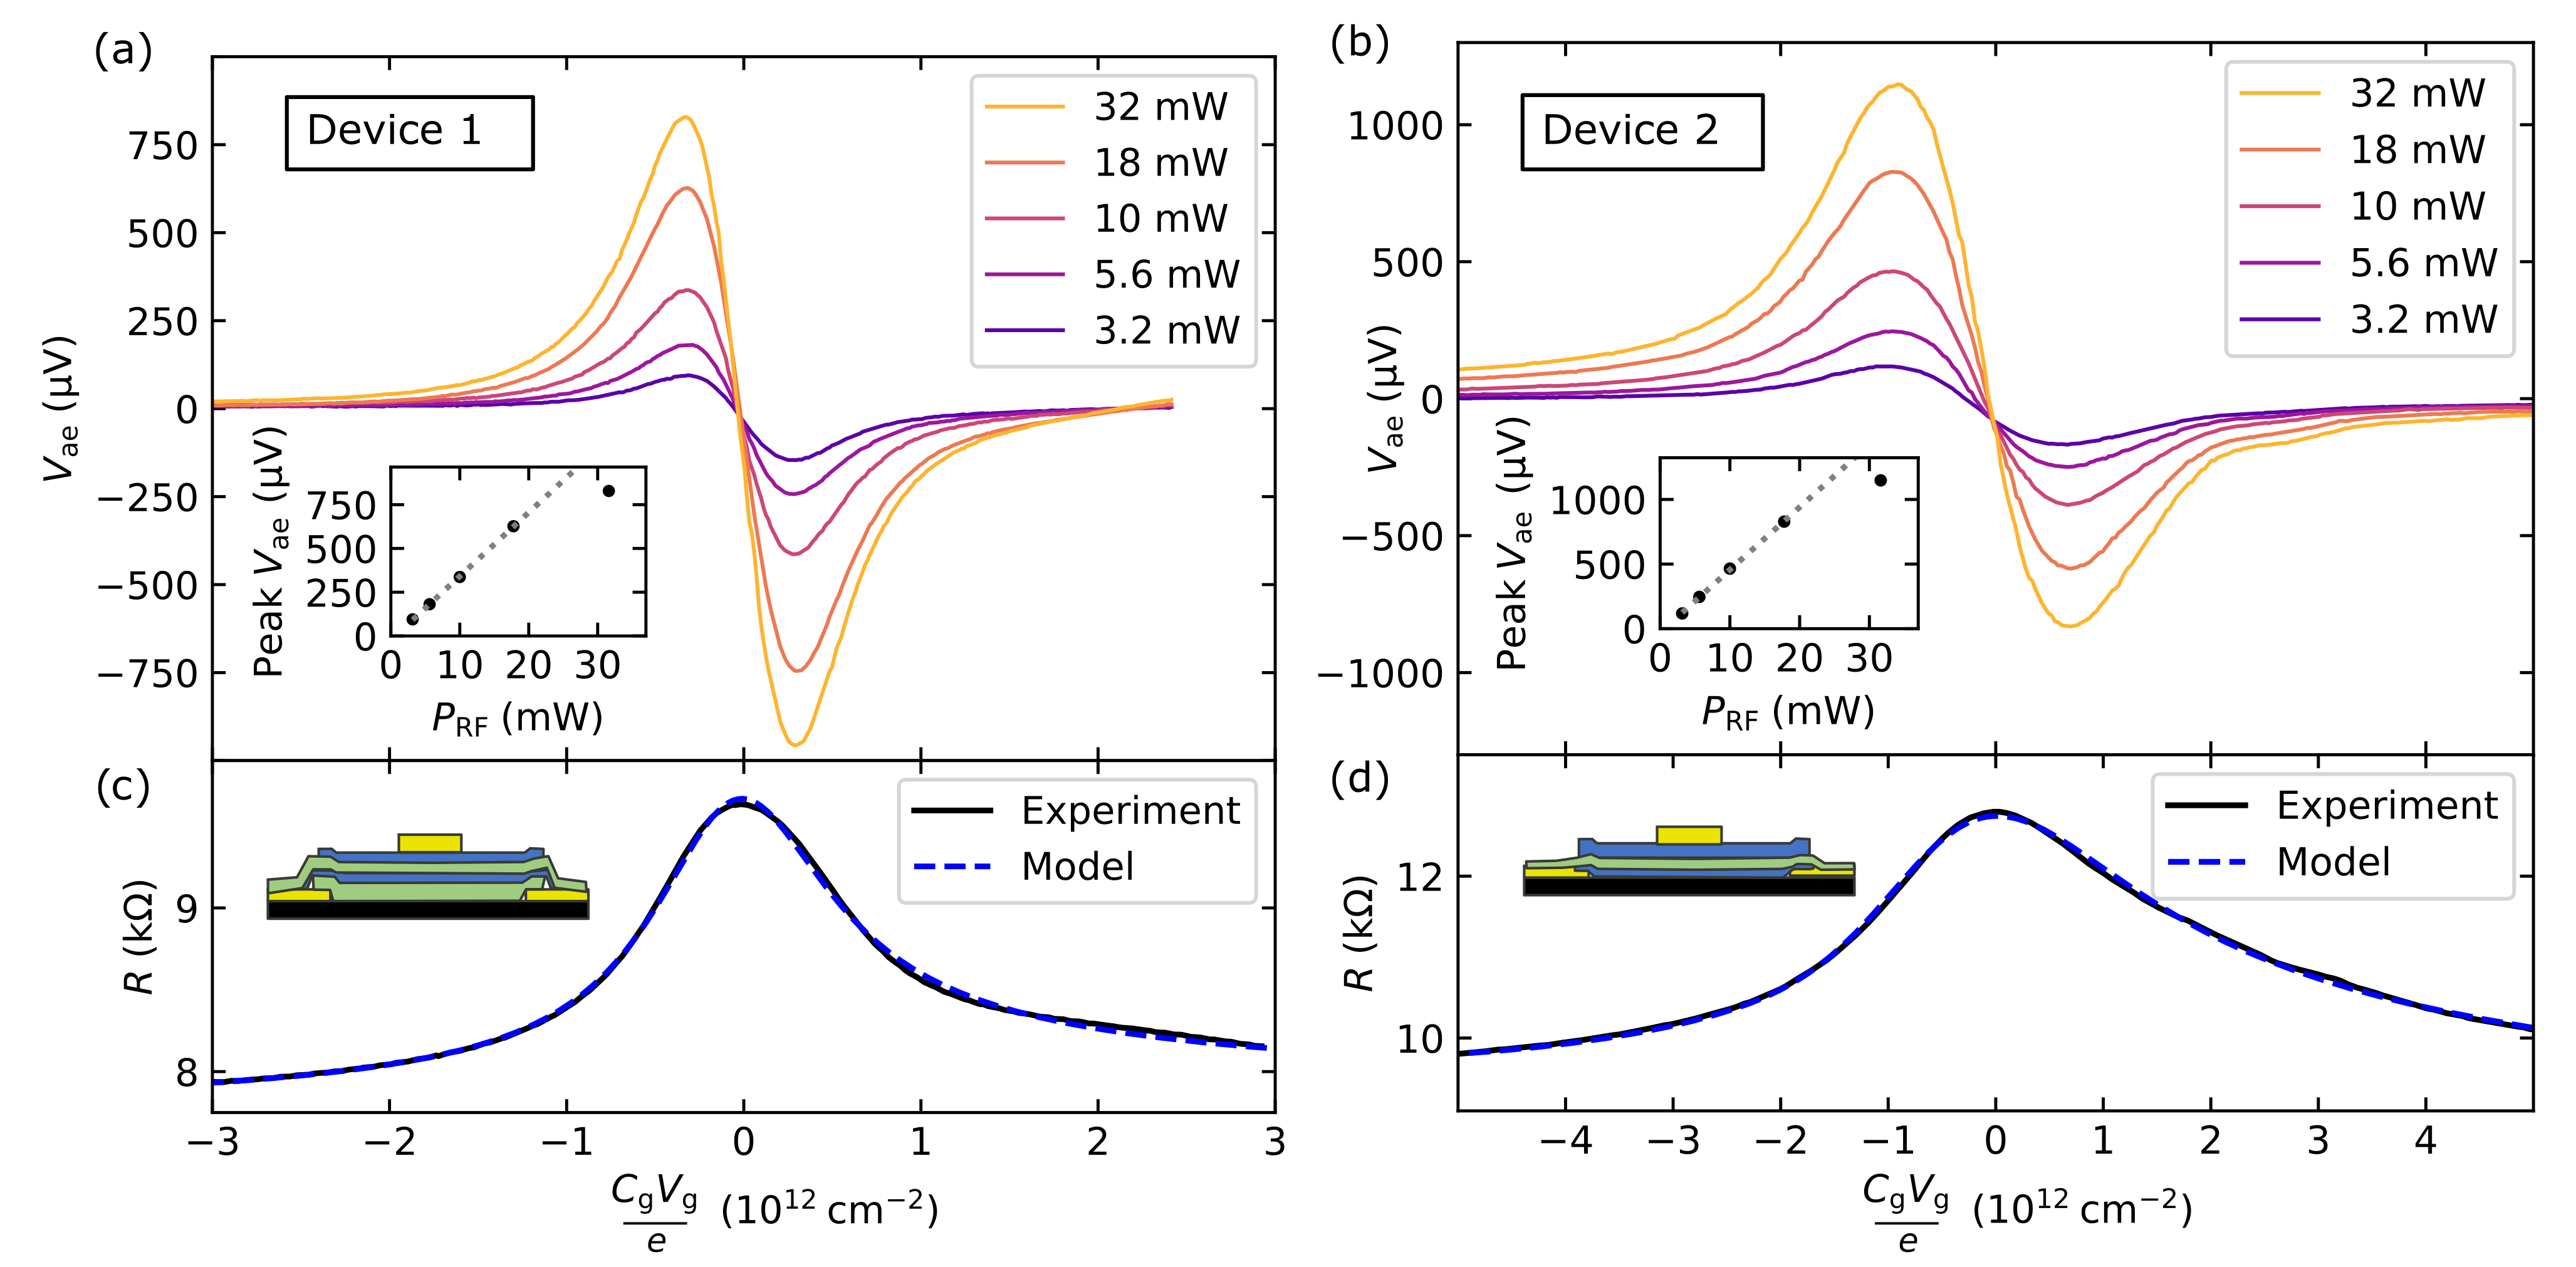
\includegraphics[width = 1\textwidth]{Figure 2, both devices AE and DC transport data.png}
    \caption{Room-temperature transport characteristics of device 1 (fully encapsulated) and device 2. (a)-(b) Acoustoelectric voltage ($V_{\mathrm{ae}}$) as a function of the carrier concentration in the graphene channel, for various levels of applied RF power $P_{\mathrm{RF}}$. $C_g$ is the gate capacitance per unit area (see Sec.\ \ref{charge pumping paper experiment design}). The inset shows the maximum $V_{\mathrm{ae}}$ as a function of $P_{\mathrm{RF}}$, with the gray dotted line as a guide for the eye. (c)-(d) Device resistance measured by setting $P_{\mathrm{RF}} = 0$ and $V_{SD} = \SI{100}{\milli\volt}$. The blue dashed line shows a fit to the experimental data. The insets show the device structures. Colors indicate LiNbO\textsubscript{3} (black), Pd (yellow), few-layer graphene (blue), and h-BN (green).}
    \label{AECP Figure 2}
\end{figure}

Figure \ref{AECP Figure 2} (c) and (d) show DC transport in devices 1 and 2, where $R = R_{\mathrm{ch}} + R_{\mathrm{C1}} + R_{\mathrm{C2}}$. With the SAW power turned off, we applied a source-drain bias $V_{SD} = \SI{100}{\milli\volt}$ and measured the DC current using a Stanford SR570 current preamplifier while sweeping $V_g$. As expected, the device resistance is largest at the CNP, where the number of free carriers is minimized. The device resistance asymptotically approaches a finite value at large $V_g$. We associate this finite resistance with a contact resistance of $R_{\mathrm{C1}} + R_{\mathrm{C2}} \approx \SI{8}{\kilo\ohm}$ for device 1 and $R_{\mathrm{C1}} + R_{\mathrm{C2}} \approx \SI{10}{\kilo\ohm}$ for device 2. Using this estimated contact resistance, we can estimate $R_{\mathrm{ch}}$ for device 1 using the equation $R_{\mathrm{ch}} \approx R - \SI{8}{\kilo\ohm}$. Similarly, $R_{\mathrm{ch}}$ for device 2 can be estimated using $R_{\mathrm{ch}} \approx R - \SI{10}{\kilo\ohm}$.

The insets of Figure \ref{AECP Figure 2} (a) and (b) show the maximum value of $V_{\mathrm{ae}}$ versus applied SAW power $P_{\mathrm{RF}}$. In both devices, we observe a linear relationship between $P_{\mathrm{RF}}$ and $V_{\mathrm{ae}}$ up to \SI{18}{\milli\watt}, which is consistent with Eq. \ref{AECP Equation 2} and has been observed in previous acoustoelectric graphene devices \cite{bandhu_macroscopic_2013}. However, at $P_{\mathrm{RF}}=\SI{32}{\milli\watt}$, the acoustoelectric voltage is smaller than expected, suggesting a nonlinear relationship between $P_{\mathrm{RF}}$ and $V_{\mathrm{ae}}$. Non-linear behavior has been observed previously in GaAs acoustoelectric devices at high SAW powers \cite{rotter_nonlinear_1999}, and suggests that the perturbation of carrier density due to the SAW is comparable in magnitude to the average carrier density in the graphene. More work is needed to understand the origin of this nonlinear relationship in acoustoelectric graphene devices. Therefore, for the analysis below, we will use the $P_{\mathrm{RF}} = \SI{18}{\milli\watt}$ data to ensure that the linear model is applicable. 

Of principal interest to this work is the shape of the peak in $V_{\mathrm{ae}}$ seen in Fig. \ref{AECP Figure 2} (a) and (b). The single-carrier, classical relaxation theory (Eqs. \ref{AECP Equation 1} and \ref{AECP Equation 2}) predicts that the acoustoelectric signal should reach a maximum when the channel conductivity $\sigma$ is equal to the characteristic conductivity of the piezoelectric substrate. For LiNbO\textsubscript{3}, this characteristic conductivity is $\sigma_c \approx (\SI{1}{\mega\ohm})^{-1}$ \cite{wixforth_surface_1989,rotter_giant_1998}. However, as can be seen in Figure \ref{AECP Figure 2} (a), the peak in $V_{\mathrm{ae}}$ occurs when $R_{\mathrm{ch}} \approx \SI{2}{\kilo\ohm}$, which corresponds to $\sigma_c \approx (\SI{2}{\kilo\ohm})^{-1}$. Prior authors noted similar discrepancies between the single-carrier theory and graphene measurements, but no quantitative description for the peak has been previously reported in literature. The peak shape can be accurately described using the mixed-carrier model outlined below.

\section{Discussion} \label{AE paper discussion}
First, we compare the magnitude of the acoustoelectric signal measured in our h-BN-encapsulated graphene device to the results of prior graphene-based acoustoelectric experiments. For device 1, $w = \SI{15}{\micro\meter}$, $R_{\mathrm{ch}} \approx \SI{2}{\kilo\ohm}$, and maximum  $V_{\mathrm{ae}} = \SI{0.98}{\milli\volt}$. If the channel was measured in a short-circuit configuration (assuming we decreased the contact resistance, such that $R_{\mathrm{C1}} + R_{\mathrm{C2}} \ll R_{\mathrm{ch}}$), we would expect $j_{\mathrm{ae}} = \SI{33}{\milli \ampere/meter}$. This current density is nearly ten times higher than previous measurements of acoustoelectric current in graphene devices \cite{bandhu_controlling_2016,okuda_acoustic_2016,tang_ultra-low_2017,okuda_graphene_2018}. For device 2, we infer $j_{\mathrm{ae}} = \SI{18}{\milli \ampere/\meter}$. The higher current density obtainable in the fully encapsulated graphene is evidence that lowering electrostatic disorder boosts acoustoelectric signals. We further quantify this insight with the model presented below.

To understand the gate-voltage dependence of $V_{\mathrm{ae}}$ in graphene devices, we consider the co-existence of electrons and holes at the CNP. In electrostatically gated graphene that has no disorder and no thermally activated charge carriers, we expect the electron and hole concentrations to be $n = C_g V_g$ for $V_g >$ 0, and $p = C_g |V_g|$ for $V_g < 0$, where $C_g$ is the gate capacitance per unit area (illustrated in Fig. \ref{AECP Figure 3} (c)). In a real graphene sample, there are thermally activated carriers and spatial fluctuations in electrostatic potential that modify the electron and hole concentrations. Figure \ref{AECP Figure 3} (a) illustrates the spatial inhomogeneity of carrier concentration in graphene \cite{martin_observation_2008}. To model this, we assume a position-dependent gate voltage offset $V_{\mathrm{offset}}(x,y)$ which has an average value 0 and standard deviation $\delta V$. We assume that the distribution of $V_{\mathrm{offset}}$ values follow a normal distribution. A similar disorder model has been used to describe the gate-dependent Hall effect in graphene \cite{brown_hall_2019}. From the function $V_{\mathrm{offset}}(x,y)$, we obtain integral forms for the spatially averaged carrier concentrations in the graphene sample (see the supplementary material) which can be solved analytically, giving

% n(V_g, \delta V) = \frac{C_g}{e}\left[\frac{V_g}{2}(1+\mathrm{erf}(\frac{V_g}{\sqrt{2}\delta V})+\frac{\delta V}{\sqrt{2\pi}}\mathrm{e}^{-\frac{V_g^2}{2\delta V^2}})\right]

\begin{equation}
    n(V_g, \delta V) = \frac{C_g}{e}\left[\frac{V_g}{2}\left(1+\mathrm{erf}\left(\frac{V_g}{\sqrt{2}\delta V}\right)\right)+\frac{\delta V}{\sqrt{2\pi}}\mathrm{exp}\left(-\frac{V_g^2}{2\delta V^2}\right)\right]
    \label{AECP Equation 3}
\end{equation}

\begin{equation}
    p(V_g, \delta V) = -\frac{C_g}{e}\left[\frac{V_g}{2}\left(1-\mathrm{erf}\left(\frac{V_g}{\sqrt{2}\delta V}\right)\right)-\frac{\delta V}{\sqrt{2\pi}}\mathrm{exp}\left(-\frac{V_g^2}{2\delta V^2}\right)\right]
    \label{AECP Equation 4}
\end{equation}
where erf is the error function, and $e$ is the electron charge. Equations \ref{AECP Equation 3} and \ref{AECP Equation 4} are plotted in Fig. \ref{AECP Figure 3} (c). In this model, the minimum carrier concentration in the graphene (the sum of $n$ and $p$ at $V_g = 0$) is 

\begin{equation}
    (n_0 + p_0) = \sqrt{\frac{2}{\pi}}\frac{C_g \delta V}{e}
    \label{AECP Equation 5}
\end{equation}

The mixed-carrier model (Eqs. 3 and 4) yields an accurate fit to the DC transport data, shown in Figure \ref{AECP Figure 2} (c) and (d). The dashed lines in Fig. 2(c) and (d) are constructed by assuming $\sigma = e\mu(n + p)$, and $R_{\mathrm{ch}} = l/(w\sigma)$, where $l$ is the length of the graphene channel (\SI{20}{\micro\meter} for both devices). For device 1 we find $\mu = \SI{7150}{\centi\meter^2/\volt\second}$ and $(n_0+p_0) =  \SI{0.38e12}{\centi\meter^{-2}}$. The minimum carrier concentration in device 1 is approaching the room-temperature limit ($\approx \SI{0.16e12}{\centi\meter^{-2}}$) which corresponds to the concentration of thermally activated charge carriers in ultraclean charge-neutral graphene \cite{xin_giant_2023}.  For device 2 we find $\mu = \SI{3500}{\centi\meter^2/\volt\second}$ and $(n_0+p_0) =\SI{0.97e12}{\centi\meter^{-2}}$. The fully encapsulated device (device 1) has higher mobility and significantly reduced charge disorder compared to device 2. 

To describe acoustoelectric voltage, we combine the mixed-carrier model (Equations. \ref{AECP Equation 3} and \ref{AECP Equation 4}) with the classical relaxation model (Eqs. \ref{AECP Equation 1} and \ref{AECP Equation 2}). The SAW pushes both electrons and holes in the same direction (Fig. \ref{AECP Figure 3}(b)). The fraction of these moving carriers which are uncompensated (carriers which do not have a partner of opposite sign) is given by $(p-n)/(p+n)$.  Using this fraction, we modify Eqs. \ref{AECP Equation 1} and \ref{AECP Equation 2}, finding the net current density from electrons and holes to be

\begin{equation}
    j_{\mathrm{ae}} = \pm \frac{\mu I}{v_{\mathrm{SAW}}}K^2\frac{\pi}{\lambda}\left[\frac{(e\mu(n+p)/\sigma_c)}{1+ (e\mu(n+p)/\sigma_c)^2}\right]\left(\frac{p-n}{p+n}\right)
    \label{AECP Equation 6}
\end{equation}
In our experiment, $e\mu(n + p) \geq \sigma_c$ at all gate voltages, therefore Eq. \ref{AECP Equation 6} simplifies to 

\begin{equation}
    j_{\mathrm{ae}} \approx \pm \frac{I \sigma_c}{e v_{\mathrm{SAW}}}K^2\frac{\pi}{\lambda}\left(\frac{p-n}{(p+n)^2}\right)
    \label{AECP Equation 7}
\end{equation}

At large $V_g$, where $n \gg p$ (or $p \gg n$), the model predicts $j_{\mathrm{ae}} \propto 1/V_g$, consistent with the single carrier model (Eq. \ref{AECP Equation 2}). Equation \ref{AECP Equation 7} can be extended to acoustoelectric voltage using the relationship $V_{\mathrm{ae}} = j_{\mathrm{ae}} w R_{\mathrm{ch}}$. At large $V_g$, the model predicts $V_{\mathrm{ae}} \propto 1/V_g^2$. Unlike the single carrier model, Eq. \ref{AECP Equation 7} is also valid at small $V_g$ where electrons and holes coexist. 

\begin{figure}
    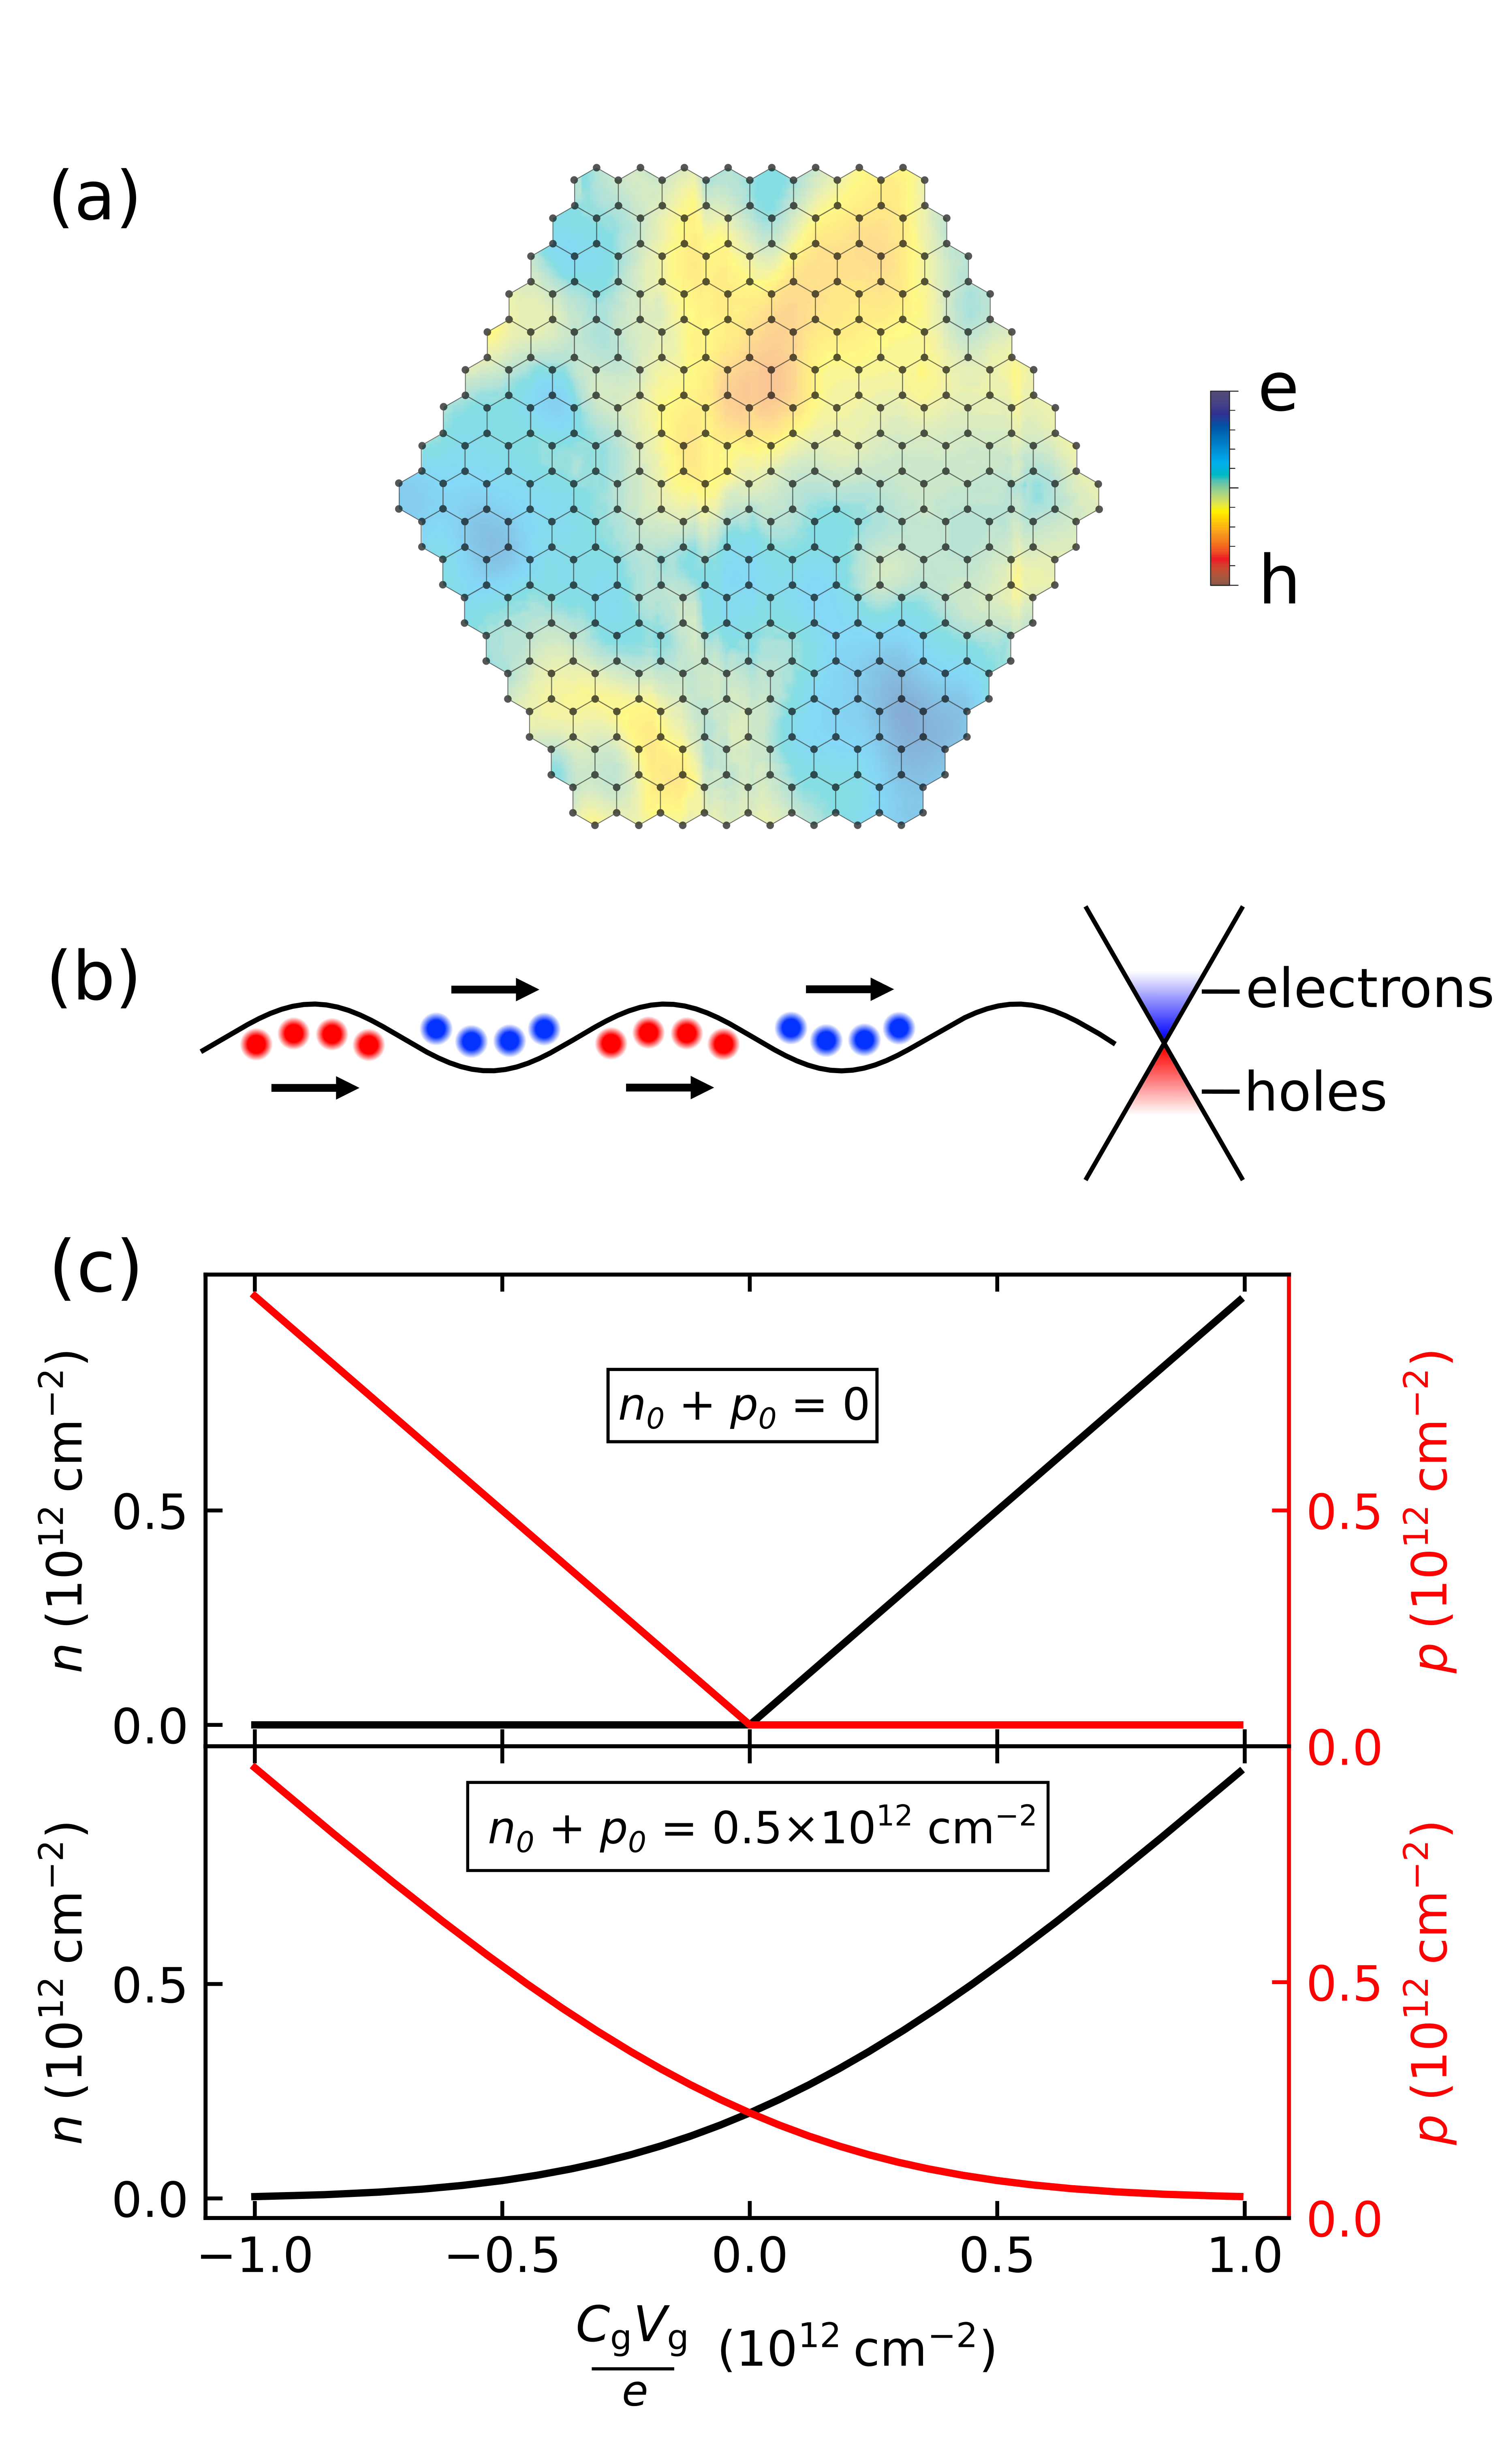
\includegraphics[width =  0.6\textwidth]{Figure 3 n and p_corrected.png}
    \caption{(a) A spatial map of electron and hole inhomogeneity in graphene. Adapted with permission from Nat. Phys. \textbf{4} 144 (2008) [27]. Copyright 2008 Springer Nature. (b) At the CNP, there are equal populations of electrons and holes. Electrons and holes are pushed in the same direction by the SAW, so there is no net acoustoelectric current. (c) Top: The electron concentration (black) and hole concentration (red) in a graphene device with no thermally activated charge carriers and no spatial fluctuation in electrostatic potential. Bottom: The electron and hole concentrations when there is a spatial fluctuation in electrostatic potential.}
    \label{AECP Figure 3}
\end{figure}

Figure \ref{AECP Figure 4} shows the excellent fit between our mixed-carrier model prediction and the measured $V_{\mathrm{ae}}$ curves. The key fitting parameter, $\delta V$, controls the width of the $V_{\mathrm{ae}}$ peaks.  For device 1 (fully encapsulated), the best fit yields $\delta V = \SI{0.65}{\volt}$, which is equivalent to $(n_0+p_0) = \SI{0.35e12}{\centi\meter^{-2}}$. For device 2, the disorder parameter is more than doubled, $(n_0+p_0) = \SI{0.88e12}{\centi\meter^{-2}}$.

\begin{figure}
    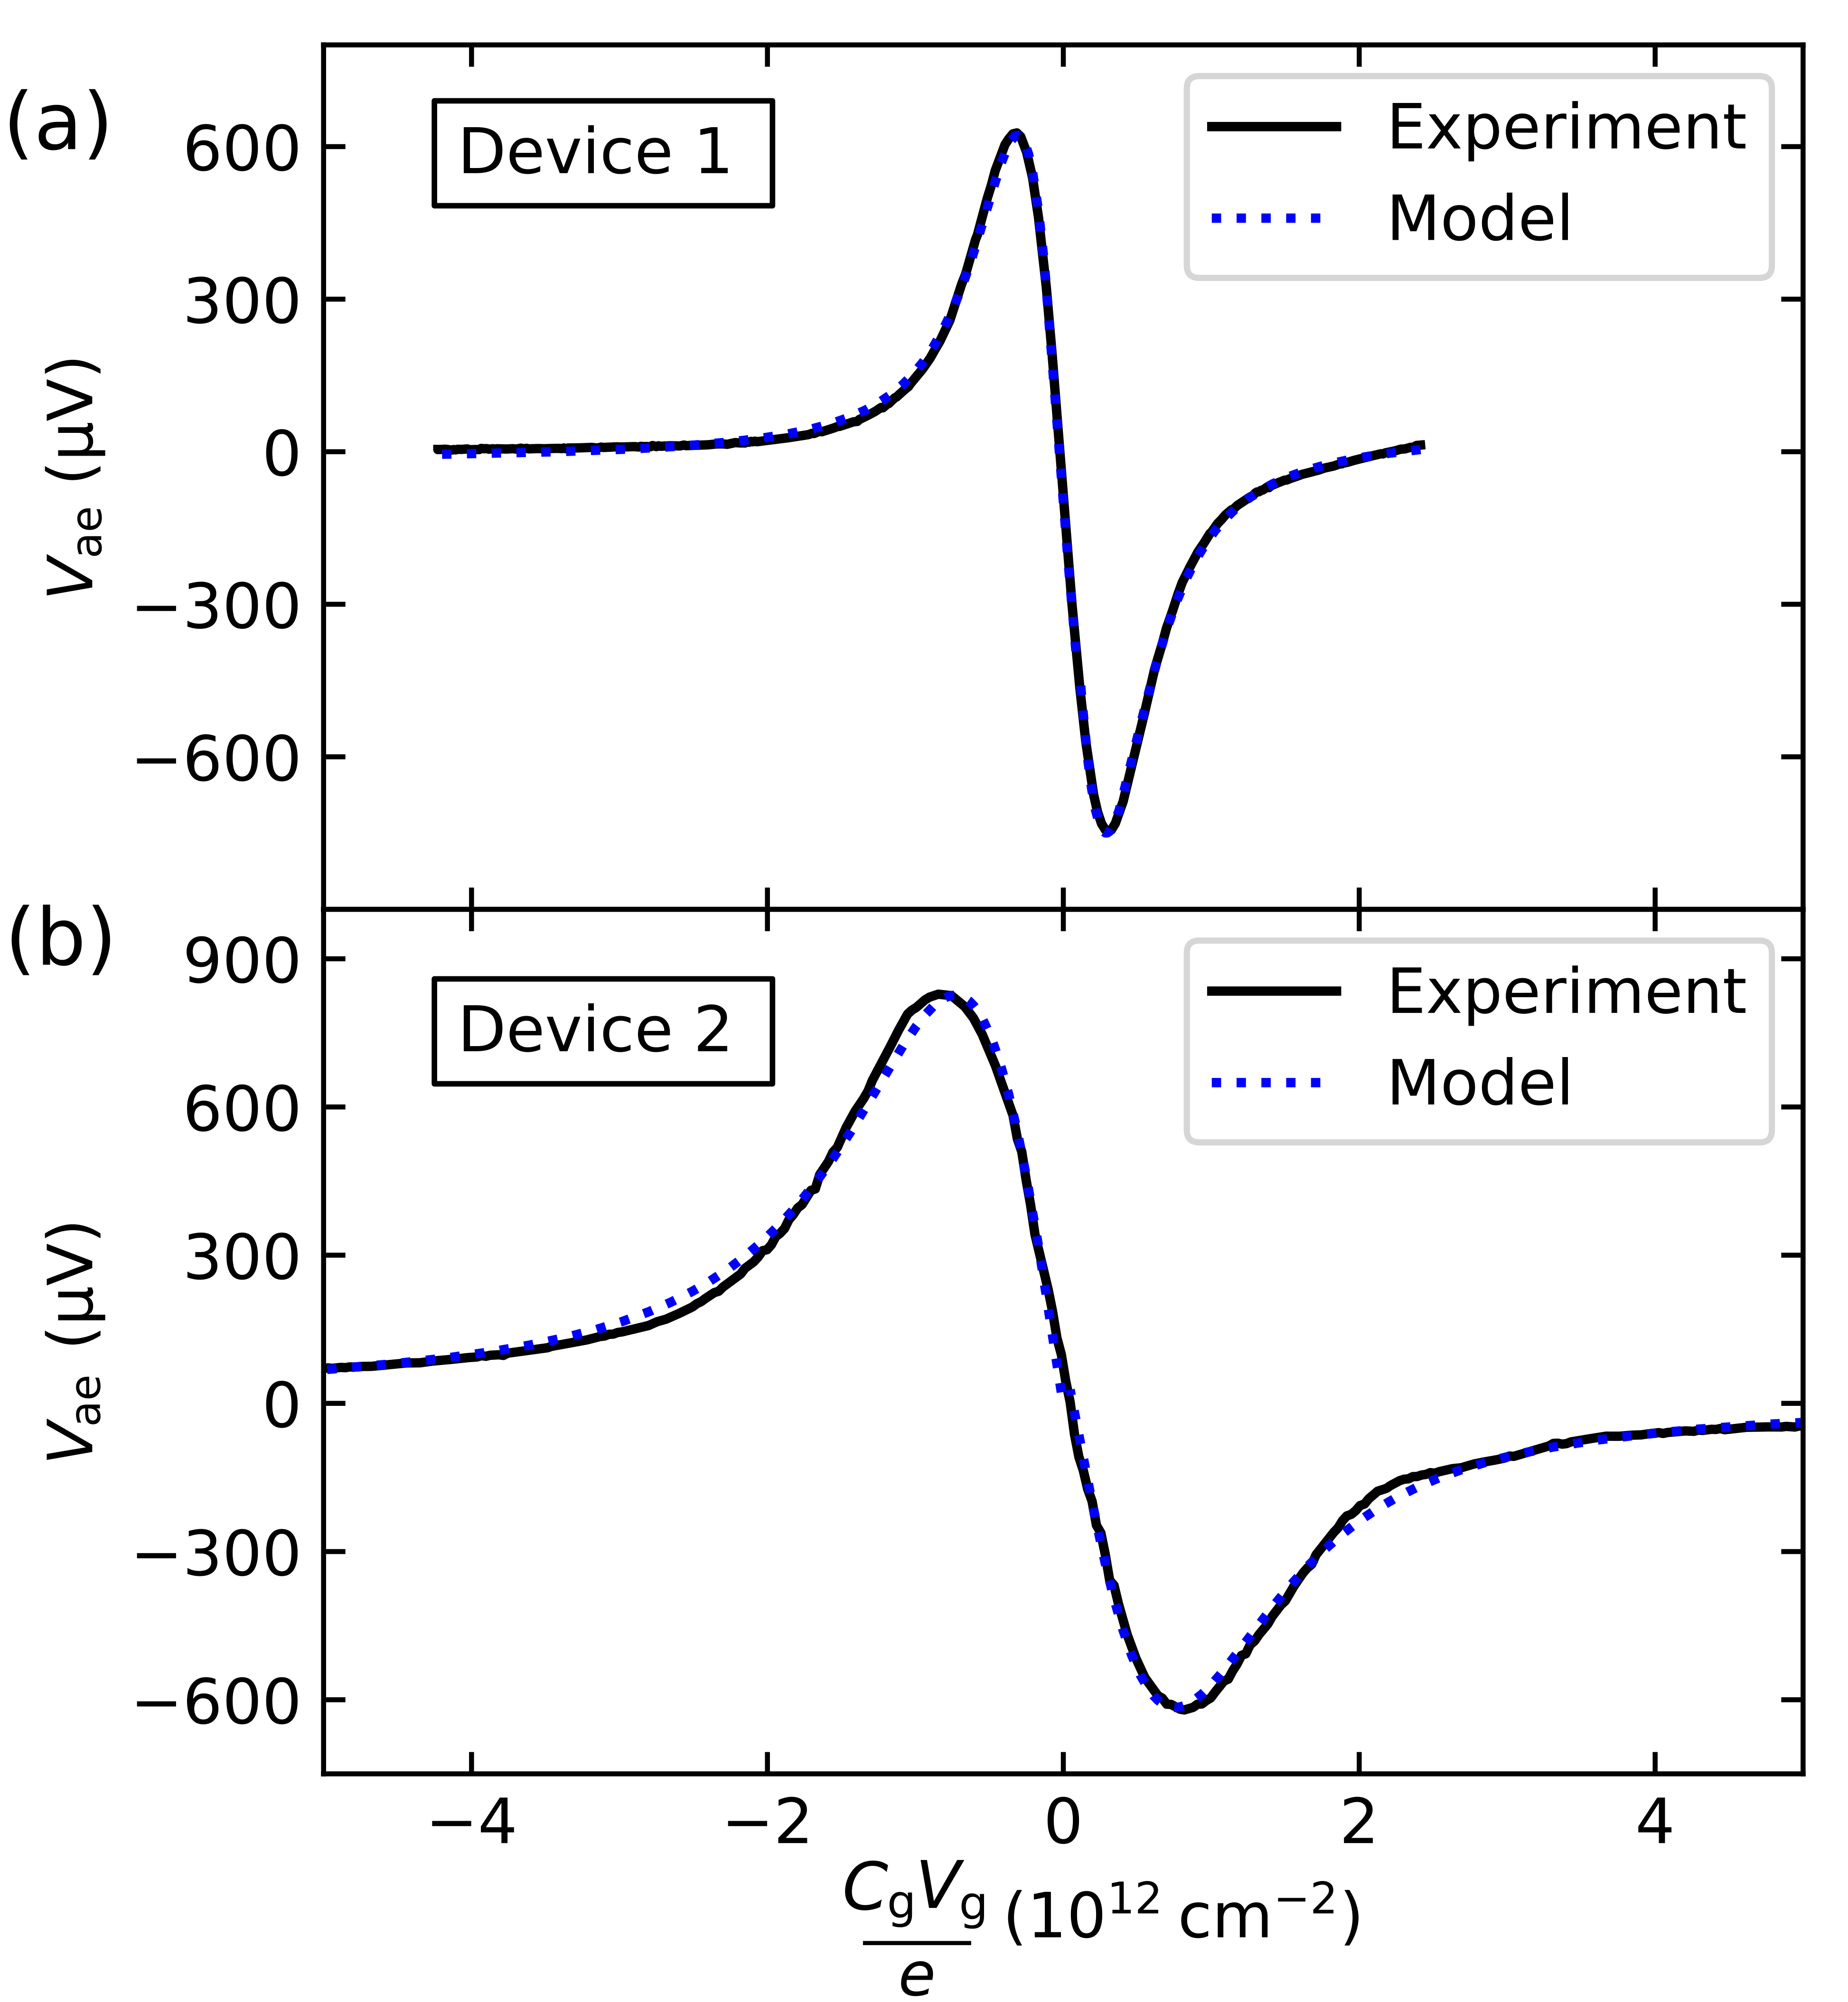
\includegraphics[width = 0.6\textwidth]{Figure 4, Both devices Fit_corrected.png}
    \caption{Mixed-carrier model (Eq. \ref{AECP Equation 7}) fit to acoustoelectric transport in the fully encapsulated (a) and half-encapsulated (b) graphene devices. This data is taken with $P_{\mathrm{RF}} = \SI{18}{\milli\watt}$.}
    \label{AECP Figure 4}
\end{figure}

The height of the $V_{\mathrm{ae}}$ peak for electron-doping differs slightly from the height of the $V_{\mathrm{ae}}$ peak for hole-doping. Therefore, we used separate fitting parameters for peak height on either side of $V_g = 0$. A similar asymmetry is found in gate-dependent Hall-effect measurements of graphene and the mechanism has been discussed extensively in literature \cite{das_sarma_electronic_2011,thiele_modeling_2010,wehrfritz_hall_2014}. Using our three-parameter fit ($\delta V$ plus two peak height parameters) we achieve excellent quantitative agreement with the experimental data.

Our mixed-carrier model (Eq. \ref{AECP Equation 6}) gives a satisfying explanation for why $\sigma \neq \sigma_c$ when $V_{\mathrm{ae}}$ is maximized in a graphene device. To maximize $V_{\mathrm{ae}}$, the gate voltage must be tuned away from $V_g = 0$ to avoid the cancellation of electron current by hole current. Conversely, if $V_g$ is too large, then $V_{\mathrm{ae}}$ decays as $1/V_g^2$. Thus, there is a sweet spot in gate voltage where most carriers have the same polarity, but carrier concentration is still small. The position of this sweet spot is determined by the disorder parameter $\delta V$. Reducing $\delta V$ will increase the height of the $V_{\mathrm{ae}}$ peak. 

The high sensitivity of $V_{\mathrm{ae}}$ with respect to $V_g$ at the CNP ($V_g = 0$) suggests that charge pumping in ultraclean graphene may be useful for sensing applications. For example, adsorption of gas molecules onto a graphene surface can modulate $\sigma$ by modulating the concentration of charge carriers in the graphene. Prior work has confirmed that changes in $\sigma$ can be used to detect adsorbed gas (reviewed in Ref.\ \cite{yang_gas_2017}). However, the $\sigma$-based transduction mechanism does not work at the CNP where $\pdv*{\sigma}{V_g} = 0$. In contrast, the acoustoelectric voltage, $V_{\mathrm{ae}}$, is most sensitive to changes in n and p when the device is operated at the CNP ($\pdv*{V_{\mathrm{ae}}}{V_g} = 0$ is maximal). Working at the CNP, gas detection events would correspond to an increase or decrease in $V_{\mathrm{ae}}$ from zero (a small signal on top of zero background), which is preferable to detecting a small change in $\sigma$ on top of a large background. Additionally, open-circuit voltage measurements circumvent unwanted noise that is generated by fluctuating contact resistance \cite{schaefer_improved_2020}. Further work in this direction could be pursued by modifying the architecture of device 1: the top side of graphene could be exposed to the environment, while the bottom side of graphene would rest on h-BN, which in turn would rest on LiNbO\textsubscript{3}.


\section{Conclusion}
We have demonstrated that the acoustoelectric signals in graphene (voltage and current) can be significantly increased by minimizing charge disorder in the graphene. h-BN-encapsulated graphene allows us to reach lower carrier concentration (close to the thermal limit) so that channel resistance better matches the optimal value to absorb SAW power. Our measurements demonstrate that room-temperature acoustoelectric current density in graphene can reach at least \SI{33}{\milli\ampere/\meter} (nearly ten times larger than previous reports). We have presented a quantitative model for the gate-dependent acoustoelectric signals that describes the coexistence regime where both electrons and holes are present. This quantitative framework will aid future SAW-based experiments designed to probe new phenomena in graphene and other 2D materials.


\section{Author contributions}

Dublin M. Nichols: Conceptualization (equal); Data curation (equal); Formal analysis (equal); Investigation (lead); Methodology (equal); Software (lead); Validation (equal); Visualization (lead); Writing \textemdash original draft (lead); Writing \textemdash review \& editing (equal). 

\noindent
Jameson G. Berg: Conceptualization (supporting); Methodology (supporting); Writing \textemdash review \& editing (supporting). 

\noindent
Takashi Taniguchi: Resources (supporting). 

\noindent
Kenji Watanabe: Resources (supporting). 

\noindent
Pallavi Dhagat: Resources (equal); Writing \textemdash review \& editing (supporting). 

\noindent
Vikram V. Deshpande: Conceptualization (supporting); Funding acquisition (equal); Methodology (supporting); Writing \textemdash review \& editing (supporting). 

\noindent
Albrecht Jander: Methodology (supporting); Resources (equal); Writing \textemdash review \& editing (supporting). 

\noindent
Ethan D. Minot: Conceptualization (equal); Formal analysis (equal); Funding acquisition (equal); Investigation (supporting); Methodology (equal); Project administration (equal); Resources (equal); Software (supporting); Supervision (lead); Visualization (supporting); Writing \textemdash original draft (supporting);Writing \textemdash review \& editing (equal)

\section{Acknowledgements}
This work was supported by the National Science Foundation under Grant No. 2004968. Part of this research was conducted at the Northwest Nanotechnology Infrastructure, a National Nanotechnology Coordinated Infrastructure site at Oregon State University which is supported in part by the National Science Foundation (grant NNCI-2025489) and Oregon State University.
K.W. and T.T. acknowledge support from the JSPS KAKENHI (Grant Numbers 21H05233 and 23H02052) and World Premier International Research Center Initiative (WPI), MEXT, Japan. 
VVD and JGB acknowledge support from the National Science Foundation under Grant No. 2005182.

\noindent\rule{\textwidth}{1pt}

\begin{center}
    This ends the peer-reviewed portion of the manuscript.
\end{center}

\noindent\rule{\textwidth}{1pt}

\clearpage
\section{Supplementary Material}

\subsection{Device images}
Figure \ref{AECP Figure S1} shows optical microscope images of device 1 (fully encapsulated) and device 2. Using tapping-mode atomic force microscopy (AFM), we measured the thickness of the channel graphene flakes to be \SI{1.2}{\nano\meter} for device 1 and \SI{1.5}{\nano\meter} for device 2.

\begin{figure}
    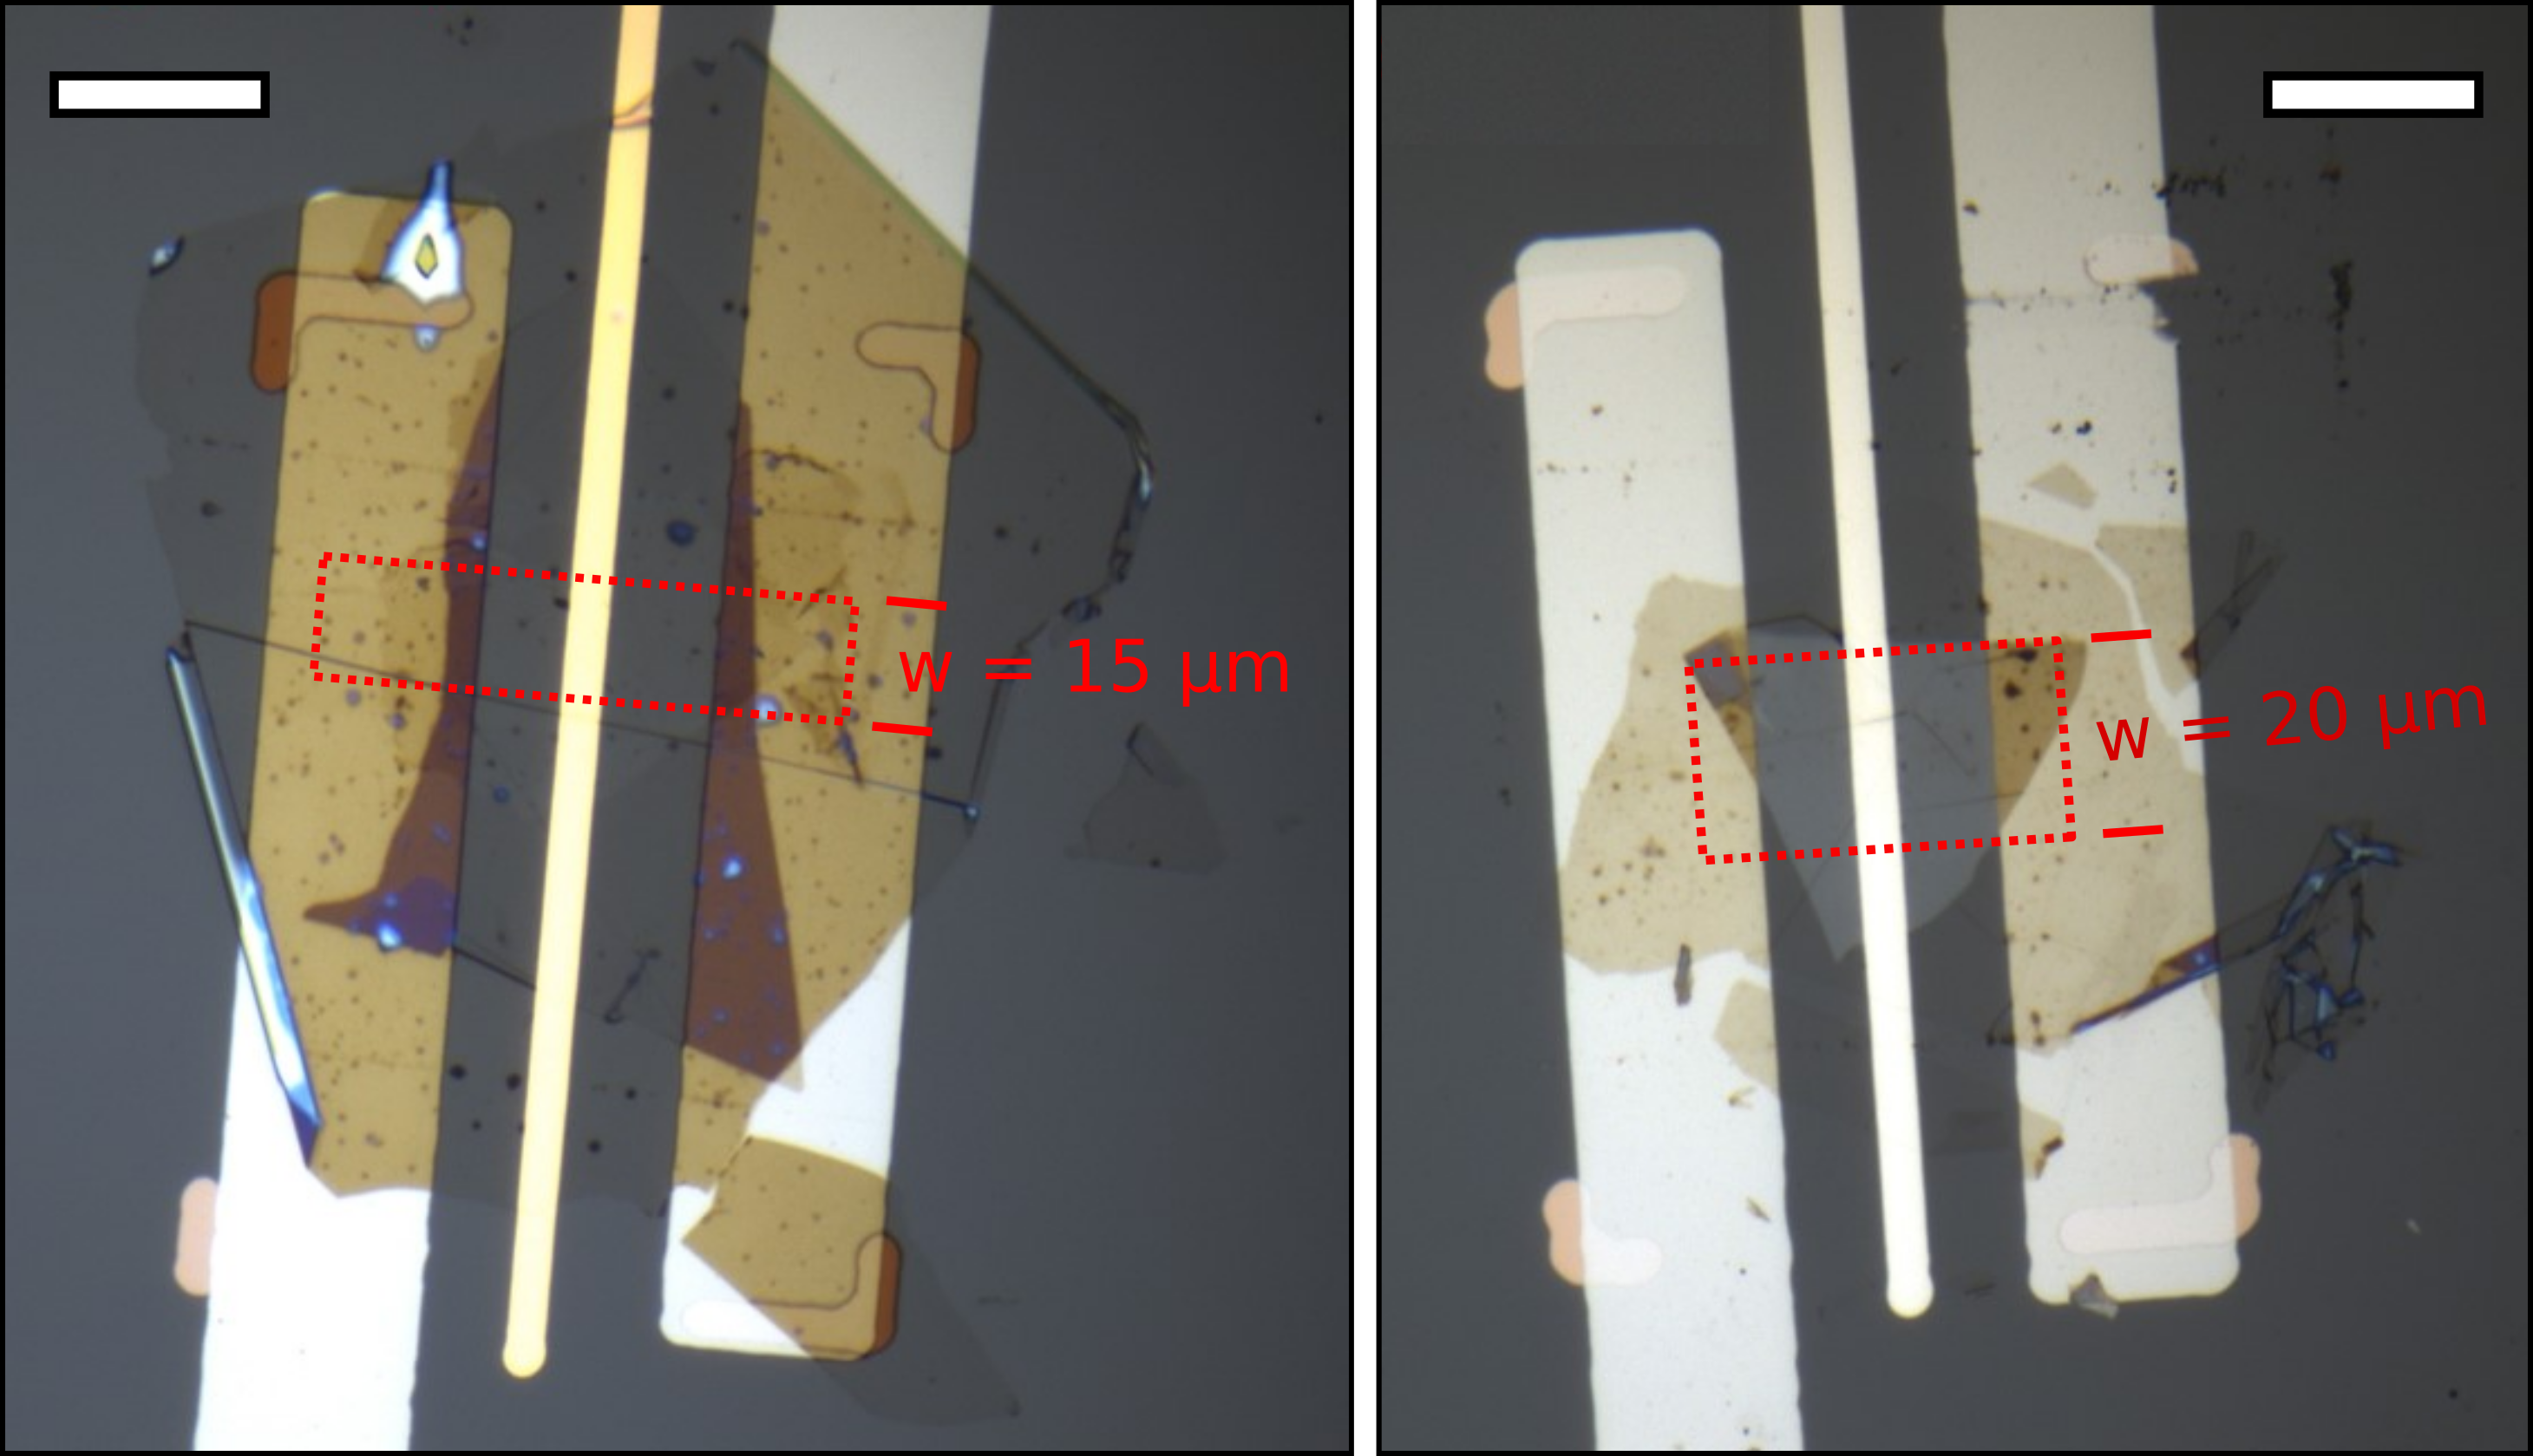
\includegraphics[width = 1\textwidth]{Figure S1, device images.png}
    \caption{Optical images of device 1 (left) and device 2 (right). Due to poor contrast of graphene on LiNbO\textsubscript{3}, we determined the approximate final location of the graphene channels from optical images taken during the transfer process. The approximate location and shape of the graphene channels are indicated with a red dotted line. Scale bar = \SI{20}{\micro\meter}.}
    \label{AECP Figure S1}
\end{figure}

\subsection{Spatially averaged carrier concentrations}
The probability of an x-y position in the graphene channel having a voltage offset
$V_{\mathrm{offset}}(x,y)$ is given by the probability distribution function

\begin{equation}
    P(V_{\mathrm{offset}}, \delta V) = \frac{1}{\sqrt{2 \pi}\delta V}\mathrm{exp}\left(-\frac{V_{\mathrm{offset}}^2}{2\delta V^2}\right)
    \label{AECP Equation S1}
\end{equation}

Using this probability distribution function, we calculate the spatially averaged carrier concentrations in the graphene channel when the global gate is set to $V_g$ to be


\begin{equation}
    n(V_g) = \frac{C_g}{e}\int_{-V_g}^{\infty}P(V_{\mathrm{offset}}, \delta V)(V_g + V_{\mathrm{offset}})dV_{\mathrm{offset}}
    \label{AECP Equation S2}
\end{equation}

\begin{equation}
    p(V_g) = \abs{\frac{C_g}{e}\int_{-\infty}^{-V_g}P(V_{\mathrm{offset}}, \delta V)(V_g + V_{\mathrm{offset}})dV_{\mathrm{offset}}}
    \label{AECP Equation S3}
\end{equation}
where $C_g$ is the gate capacitance per unit area. The lower limit of integration in Eq. \ref{AECP Equation S2} corresponds to the lowest value of $V_{\mathrm{offset}}$ that still gives electron doping (see Fig. \ref{AECP Figure S2}). Similarly, the upper limit of integration in Eq. \ref{AECP Equation S3} corresponds to the highest value of $V_{\mathrm{offset}}$ that still gives hole doping.

\begin{figure}
    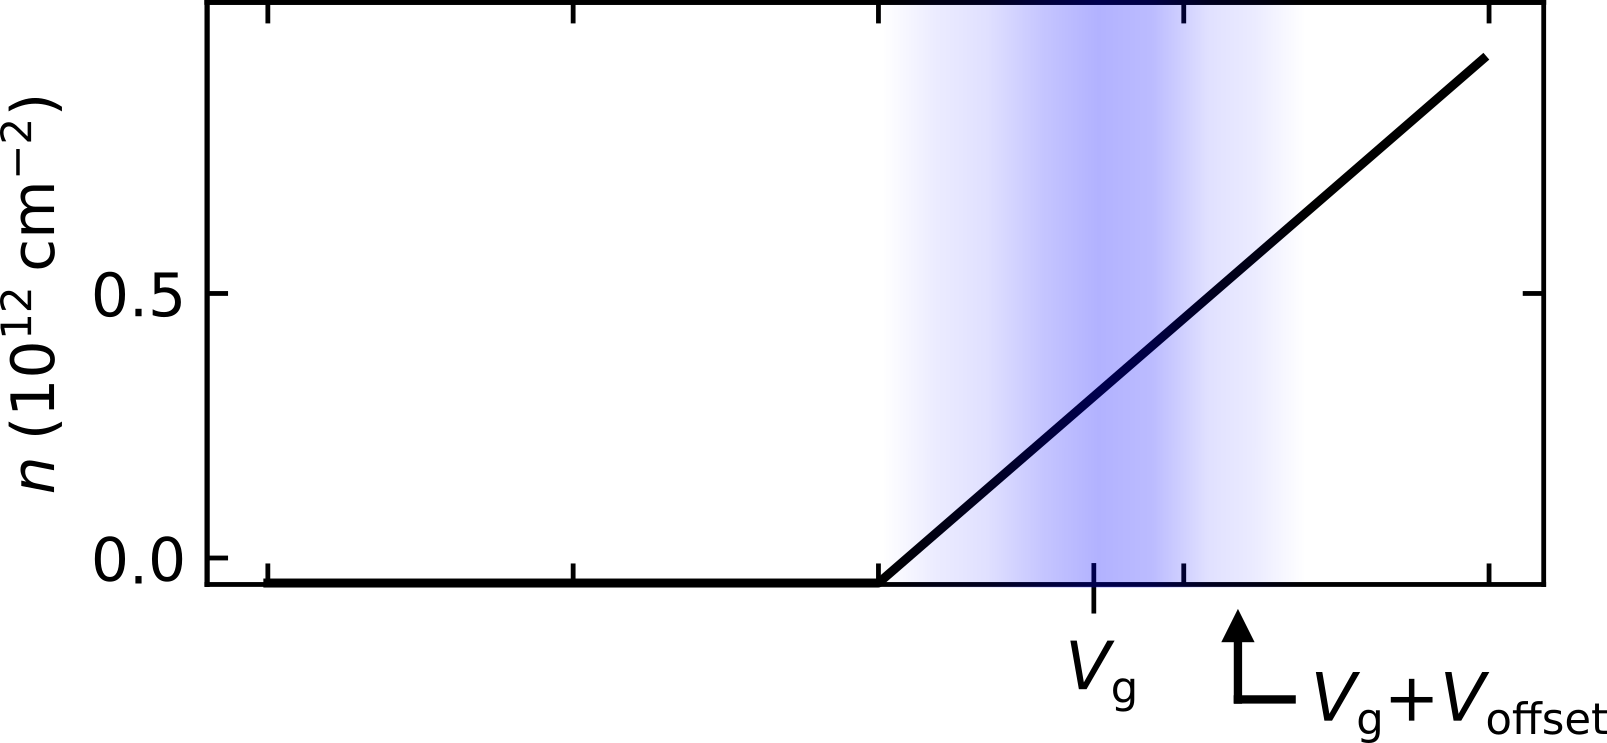
\includegraphics[width = 0.5\textwidth]{Figure S2, V_offset.png}
    \caption{Calculating the spatially averaged electron concentration. The average gate voltage is $V_g$, and the local gate voltage is $V_g + V_{\mathrm{offset}}$. The distribution of local gate voltages (depicted with blue shading) has a standard deviation $\delta V$. When $V_g + V_{\mathrm{offset}} < 0$, the location does not contribute to electron concentration.}
    \label{AECP Figure S2}
\end{figure}

\subsection{SAW device characterization; measurement of acoustoelectric current} 
Figure \ref{AECP Figure S3} shows acoustoelectric current ($I_{ae}$) and reflected SAW power $S_{11}$ as a function of frequency in device 2, measured using an Agilent E5071C-280 vector network analyzer. We observe a SAW resonance in $S_{11}$ at \SI{170}{\mega\hertz}, close to our designed frequency of \SI{170}{\mega\hertz}.  $I_{ae}$ closely follows the drop in $S_{11}$, confirming the dependence of our measured acoustoelectric signals ($I_{ae}$ and $V_{\mathrm{ae}}$) on transmitted SAW power. The interdigitated transducers in device 1 and device 2 are identical.

\begin{figure}
    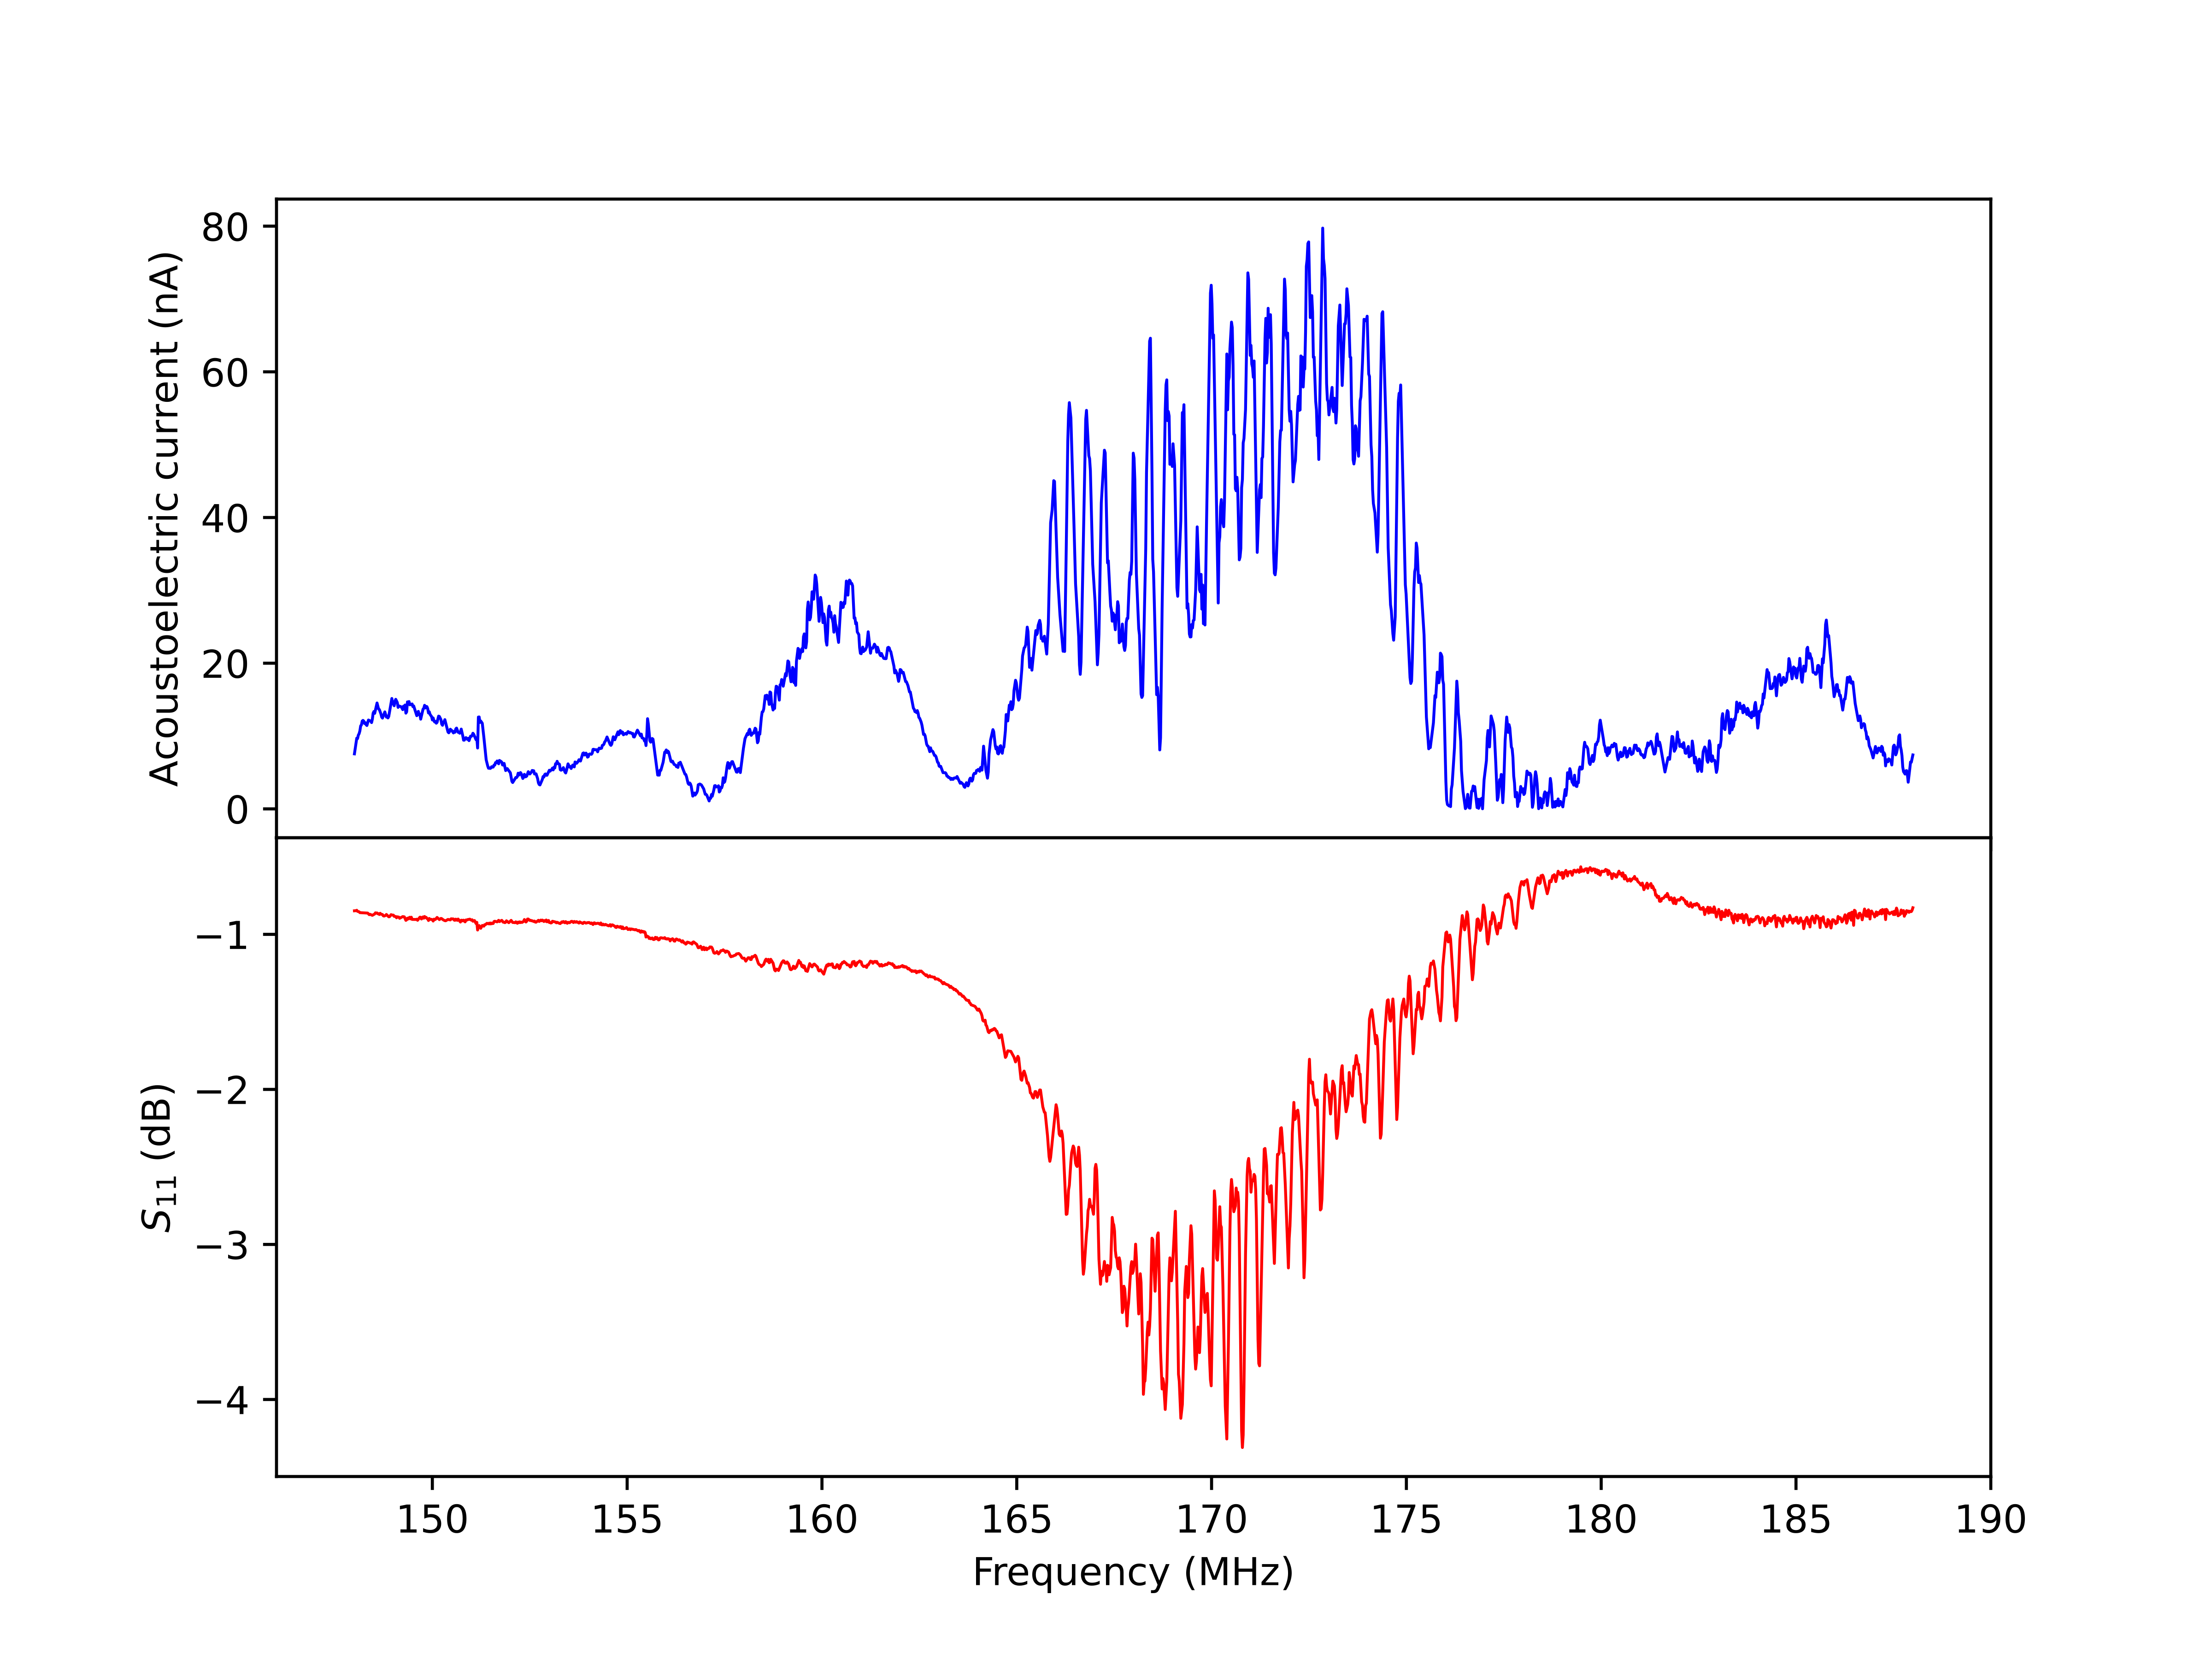
\includegraphics[width = 1\textwidth]{Figure S3, AEC vs S11.png}
    \caption{Acoustoelectric current (top) and $S_{11}$ (bottom) as a function of frequency in device 2.}
    \label{AECP Figure S3}
\end{figure}

\subsection{Comparing pumped current density of prior acoustoelectric graphene devices}

Ref.\ \cite{okuda_graphene_2018}: $I_{ae} = \SI{17}{\micro \ampere}, w = \SI{5}{\milli\meter}: \SI{3.4}{\milli \ampere/\meter}$

\noindent
Ref.\ \cite{okuda_acoustic_2016}: $I_{ae} = \SI{5}{\micro \ampere}, w = \SI{5}{\milli\meter}: \SI{1}{\milli \ampere/\meter}$

\noindent
Ref.\ \cite{tang_ultra-low_2017}: $I_{ae} = \SI{0.1}{\micro \ampere}, w = \SI{80}{\micro\meter}: \SI{1.25}{\milli \ampere/\meter}$

\noindent
Ref.\ \cite{bandhu_controlling_2016}: $I_{ae} = \SI{10}{\nano \ampere}, w = \SI{3}{\milli\meter}: \SI{0.0033}{\milli \ampere/\meter}$


\section{Nonlinear acoustoelectric effect in graphene} \label{nonlinear acoustoelectric effect}

In this work, we found that, above $P_{\mathrm{RF}} = \SI{18}{\milli\watt}$, the relationship between peak $V_{\mathrm{ae}}$ and $P_{\mathrm{RF}}$ becomes sublinear. This has been observed before in charge pumping experiments in GaAs/AlGaAs quantum wells \cite{rotter_charge_1999,rotter_nonlinear_1999}. In those experiments, the nonlinearity at large SAW powers was attributed to the local perturbation of carrier density by the SAW being larger than the local carrier concentration (see Sec.\ \ref{classical relaxtion model}). In this nonlinear regime, the charge carriers are completely trapped in the SAW potential and flow as stripes moving at the speed of sound.

To further investigate the nonlinear acoustoelectric charge pumping in graphene, we took measurements of acoustoelectric voltage $V_{\mathrm{ae}}$ versus gate voltage $V_g$ at finer steps of $P_{\mathrm{RF}}$. Using a Stanford SG382 function generator, we drove the interdigitated transducer of device 1 (fully encapsulated) with a $\SI{170}{\mega\hertz}$ signal pulsed at $\SI{100}{\hertz}$. We measured the generated acoustoelectric voltage $V_{\mathrm{ae}}$ using an SR830 lock-in amplifier. The $\SI{100}{\hertz}$ pulse signal is applied by the SR830, allowing us to lock in to the $V_{\mathrm{ae}}$ signal. Figure \ref{AEV nonlinear series} shows $V_{\mathrm{ae}}$ versus carrier density $V_g$ for device 1.

\begin{figure}
    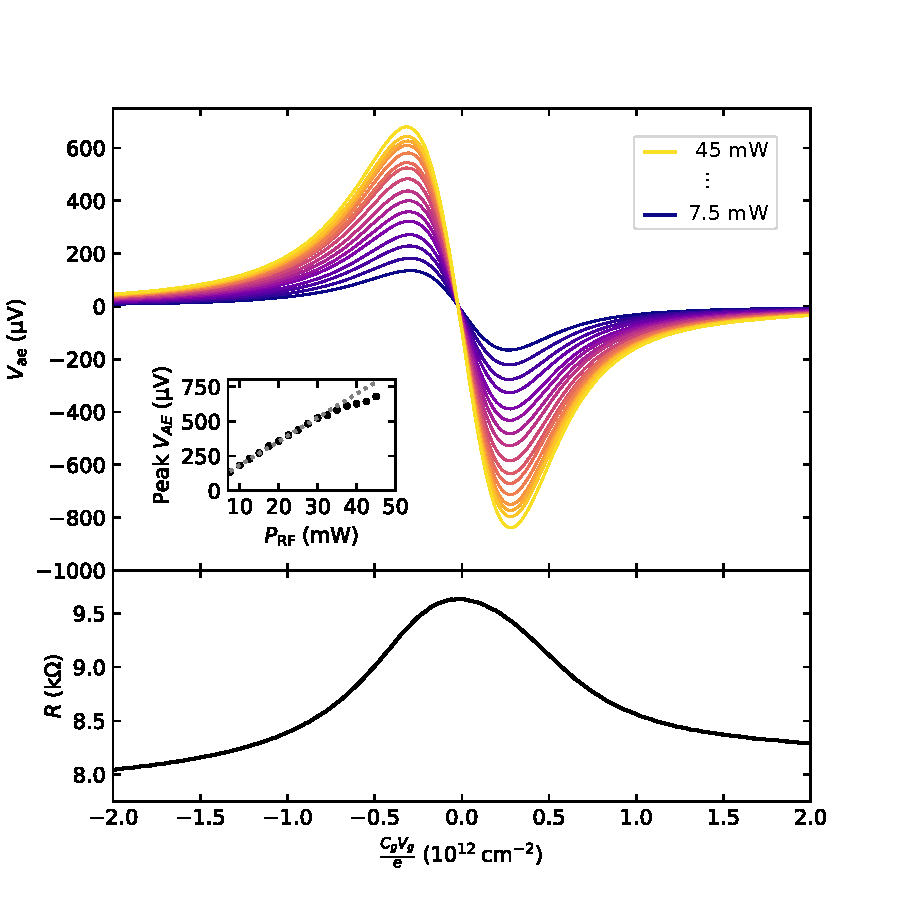
\includegraphics{AEV V3 power series plot_output.pdf}
    \caption{Room-temperature transport characteristics of device 1 (fully encapsulated). (a) Acoustoelectric voltage ($V_{\mathrm{ae}}$) as a function of carrier density in the graphene channel, for various levels of applied RF power $P_{\mathrm{RF}}$ (b) Resistance of device 1 versus gate voltage $V_g$ measured by setting $P_{\mathrm{RF}} = 0$ and $V_{SD} = \SI{100}{\milli\volt}$.}
    \label{AEV nonlinear series}
\end{figure}
The measured peak in $V_{\mathrm{ae}}$ continues to be sublinear up to $P_{\mathrm{RF}} = \SI{45}{\milli\watt}$ (the maximum that we can achieve with the SG382 function generator). Unfortunately, in our experiment, the range of $P_{\mathrm{RF}}$ that we can achieve does not extend far enough into the nonlinear regime to compare to the model presented in Ref.\ \cite{rotter_nonlinear_1999}. In future experiments, there are multiple methods that could be used to achieve higher SAW power and reach further into the nonlinear regime. The encapsulated graphene could be put closer to the interdigitated transducer to increase the SAW intensity at the graphene. The impedance of the IDT could be better matched to the function generator to convert more $P_{\mathrm{RF}}$ into SAW power. Or, a function generator with a higher power limit could be used.

The threshold for the nonlinear regime occurs when the local perturbation of carrier density by the SAW is larger than the local carrier concentration. Therefore, the $P_{\mathrm{RF}}$ at which $V_{\mathrm{ae}}$ versus $P_{\mathrm{RF}}$ becomes sublinear should change with changing carrier concentration. Figure \ref{vae vs prf at different vg} shows $V_{\mathrm{ae}}$ versus $P_{\mathrm{RF}}$ for different values of $V_g$. 
\begin{figure}
    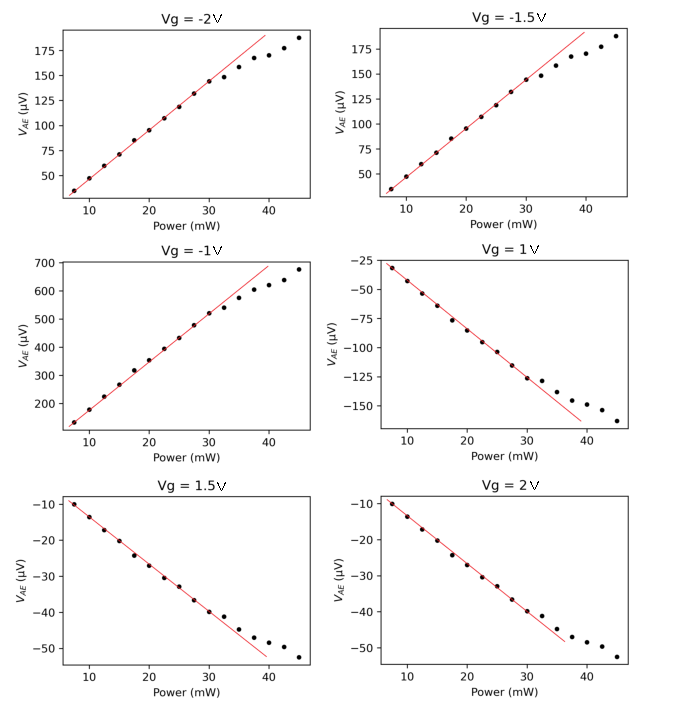
\includegraphics[width = 1\textwidth]{vae prf nonlinear at different vg.pdf}
    \caption{Cross-sections of $V_{\mathrm{ae}}$ versus $P_{\mathrm{RF}}$ at various values of $V_g$. The red lines serve as a guide for the eye.}
    \label{vae vs prf at different vg}
\end{figure}
Though we achieve a $4\times$ change in carrier concentration ($0.5$ to $\SI{2.0E12}{\centi\meter^{-2}}$), we do not observe a difference in the $P_{\mathrm{RF}}$ nonlinear threshold as carrier concentration is varied. One possible explanation is that, since we have few-layer graphene (likely bilayer from AFM thickness measurement), the static gate tunes the carrier density in the top graphene layer more strongly, and the SAW tunes the carrier density in the bottom graphene layer more strongly. Future experiments on charge pumping in monolayer graphene would help improve our understanding of how multiple graphene layers plays a role in the nonlinear acoustoelectric effect.

Reference \cite{rotter_nonlinear_1999} observed in their experiment on nonlinear acoustoelectric charge pumping in GaAs/AlGaAs quantum wells that the electron concentration at which $V_{\mathrm{ae}}$ is maximized increases at increasing $P_{\mathrm{RF}}$. Figure \ref{Vg at which vae is max or min} illustrates the location of the maximum/minimum in $V_{\mathrm{ae}}$ at varying $P_{\mathrm{RF}}$. I fit each peak/trough in $V_{\mathrm{ae}}$ to a polynomial to find the precise location of the maximum/minimum in $V_{\mathrm{ae}}$. As $P_{\mathrm{RF}}$ increases, we do observe an increase in the value of $|V_g|$ at which $V_{\mathrm{ae}}$ is maximized or minimized.

\begin{figure}
    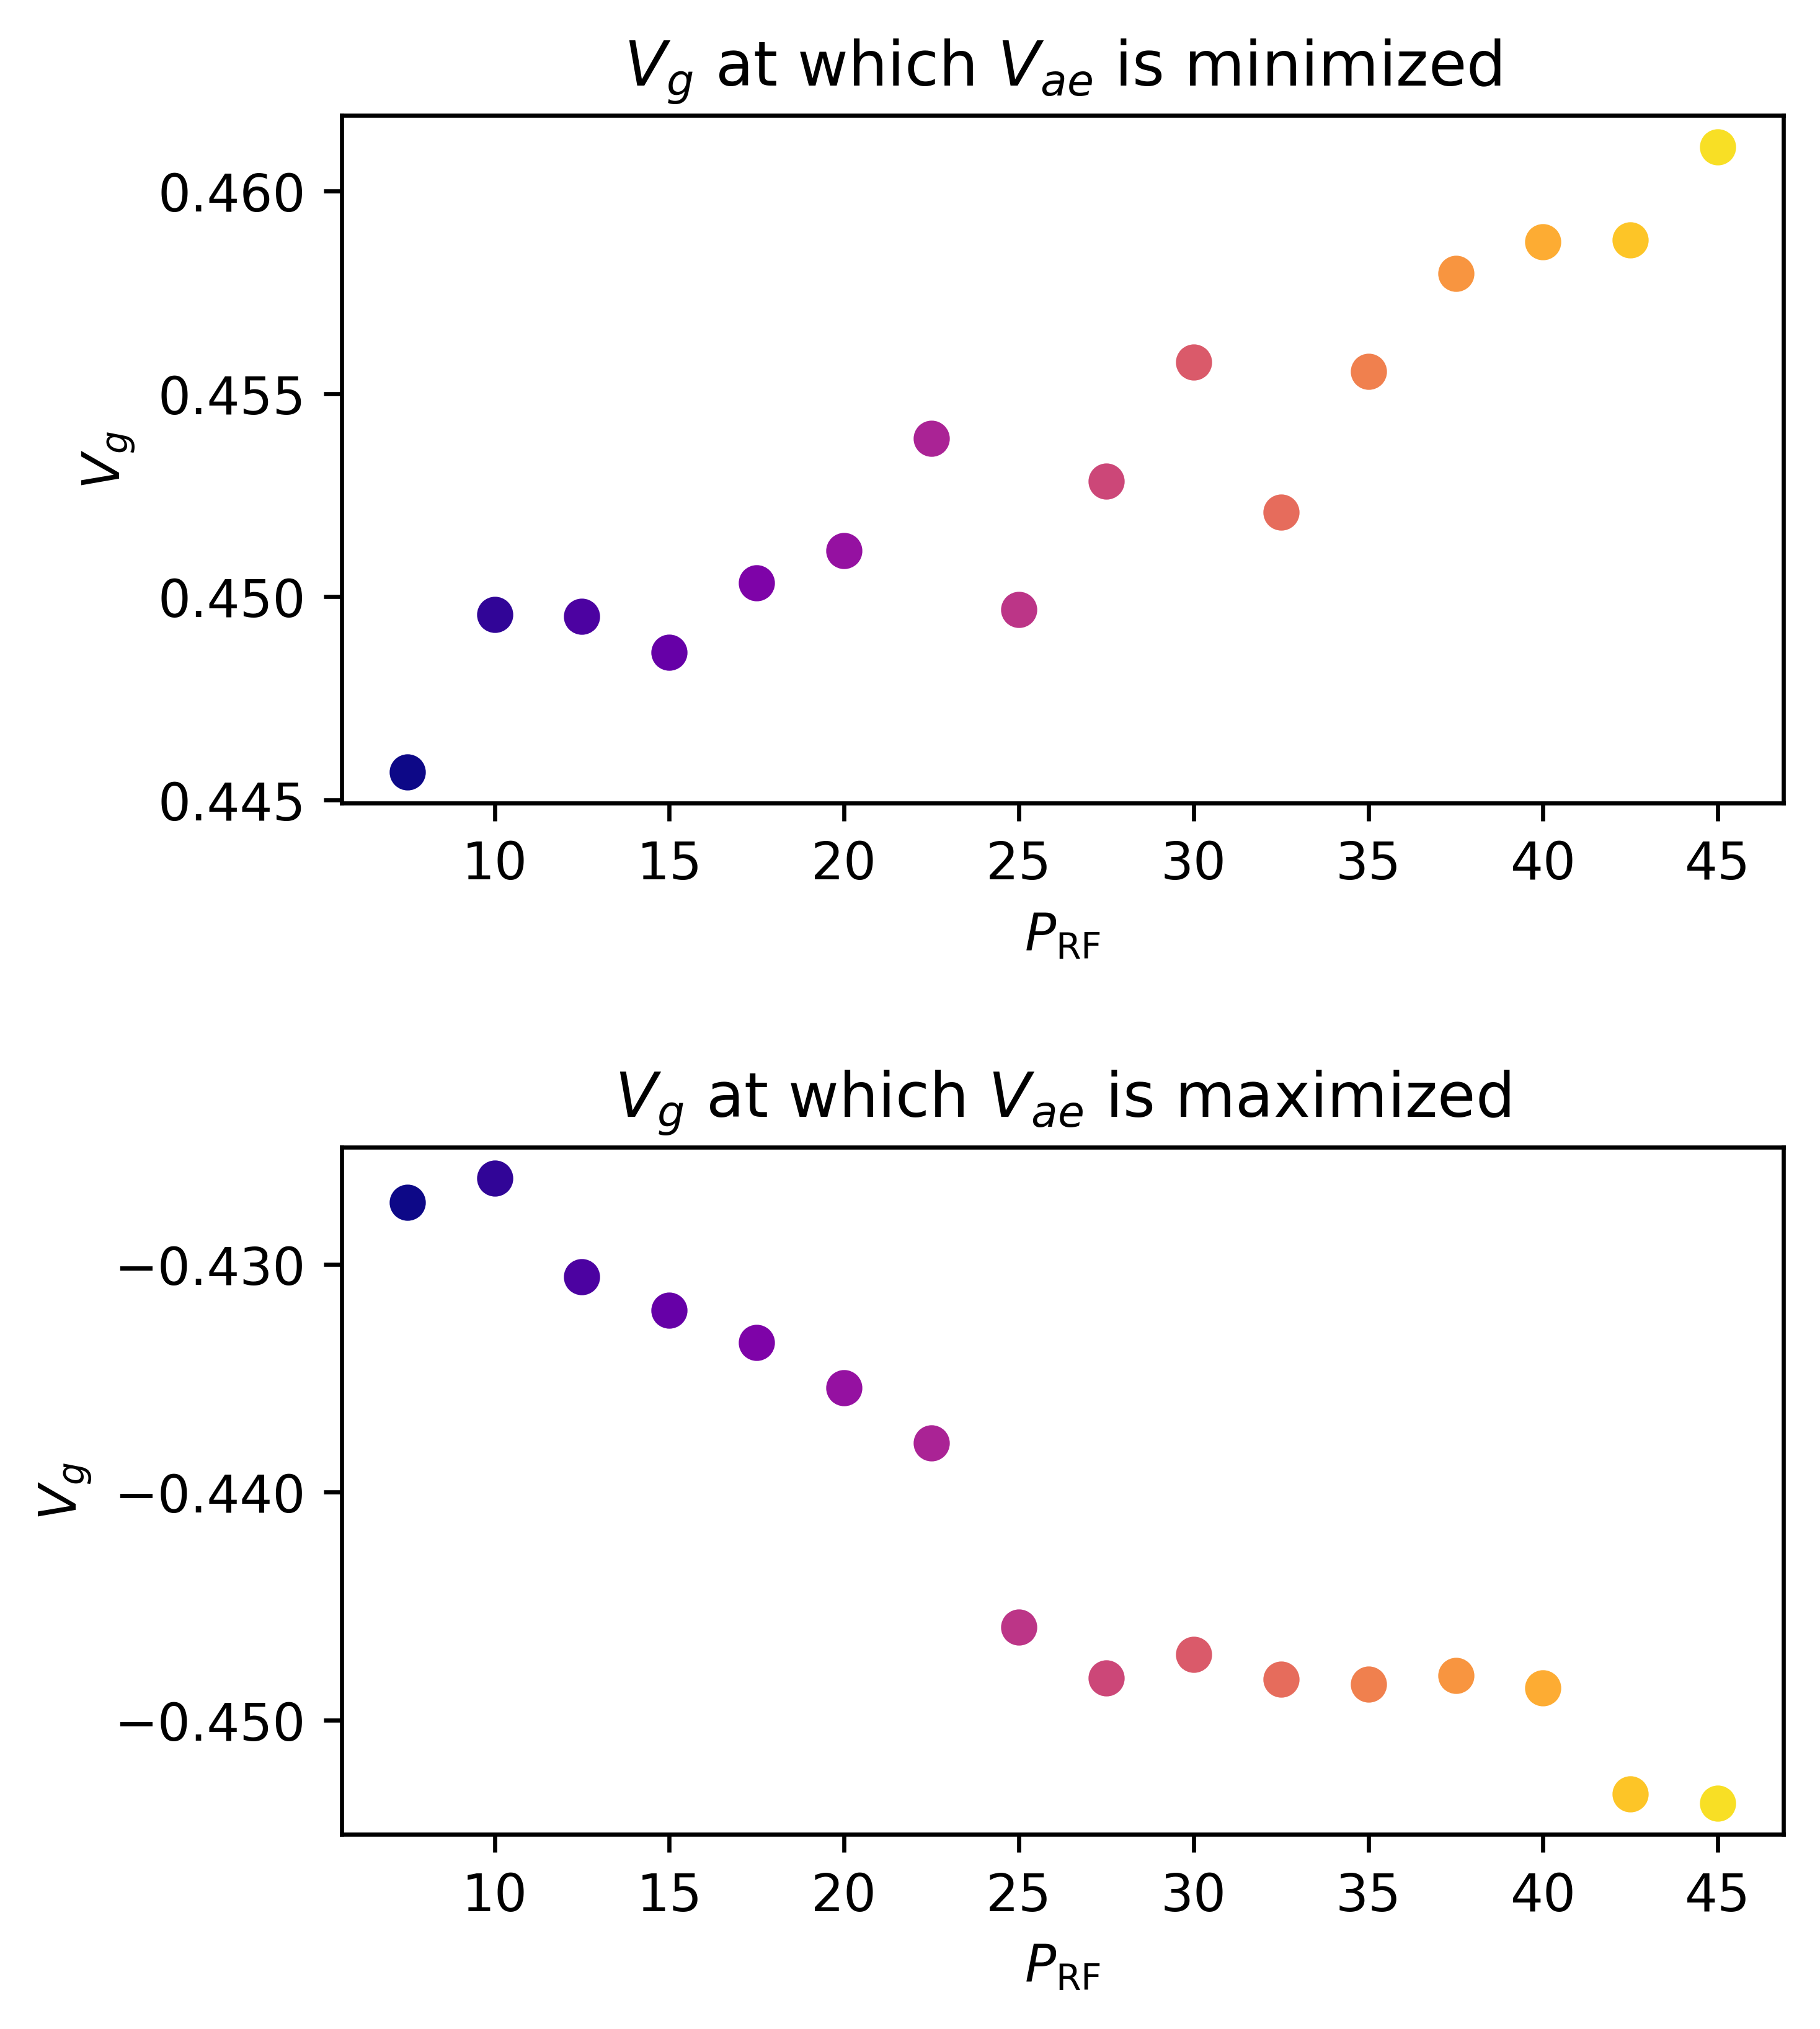
\includegraphics{Vg at which vae is max or min.png}
    \caption{Gate voltage $V_g$ for which $V_{\mathrm{ae}}$ is maximized (top, hole transport) or minimized (bottom, electron transport). The location of the peak $V_{\mathrm{ae}}$ moves to higher $|V_g|$ (higher carrier concentration) as $P_{\mathrm{RF}}$ increases. The data has been shifted on the $V_g$-axis to align the CNP with $V_g$ = 0.}
    \label{Vg at which vae is max or min}
\end{figure}


These preliminary results on nonlinear charge pumping in graphene suggest that we achieve a perturbation in carrier density by the SAW which is larger than the local carrier density in the graphene. This bodes well for future experiments towards topological charge pumping in carbon nanotubes, which require electrons to be completely trapped in the SAW potential. However, more work is needed to form a complete picture of the nonlinear acoustoelectric effect in graphene. Future experiments which measure at higher $P_{\mathrm{RF}}$ would allow us to directly fit the model presented by Ref.\ \cite{rotter_nonlinear_1999}. Also, measurements of charge pumping in monolayer graphene would allow us to assess the role that multiple graphene layers plays in acoustoelectric charge pumping. 

This nonlinear charge pumping regime, in which electrons are trapped in the SAW potential wells, and holes in the SAW potential peaks, is reminiscent of the charge and spin density waves observed in other quantum materials \cite{rahnejat_charge_2011,pasztor_multiband_2021}. These stripe phases are predicted to give rise to further exotic electronic states, such as liquid crystal states \cite{fradkin_liquid-crystal_1999}. In future experiments, charge pumping in the nonlinear regime could be used to create a dynamic, tunable charge density wave, realizing acoustically-induced exotic ordered electron phases, similarly to the acoustically-induced Hall effect observed previously in graphene \cite{zhao_acoustically_2022}. 


% ~~~~~~~~~Flip-chip chapter~~~~~~~~~~
\chapter{Flip-chip design for coupling surface acoustic waves to quantum materials} \label{flip-chip chapter}

\section{Introduction}

For some quantum materials, there are unique requirements for device fabrication that make it challenging to integrate surface acoustic waves (SAWs) into the device. For example, carbon nanotube (CNT) growth requires temperatures in excess of \SI{800}{\celsius}, which will damage the delicate interdigitated fingers of a SAW device. Figure \ref{IDT damaged} shows an IDT with $\lambda = \SI{240}{\nano\meter}$ (metallized with 3/\SI{17}{\nano\meter} Cr/Pt) before and after a CNT growth. Just 5 minutes at \SI{800}{\celsius} destroyed the thin interdigitated fingers, even though the melting point of Pt is over \SI{1700}{\celsius}. This could be avoided by growing CNTs on a separate substrate, encapsulating the CNT in hexagonal boron nitride (h-BN), and transferring the CNT next to a SAW device. However, CNTs are invisible in an optical microscope, making encapsulation challenging. Furthermore, the CNTs would pick up contamination from the growth substrate, which would subsequently be trapped between the h-BN layers. Therefore, I desire to investigate alternative methods of interfacing a CNT with a SAW.

\begin{figure}
    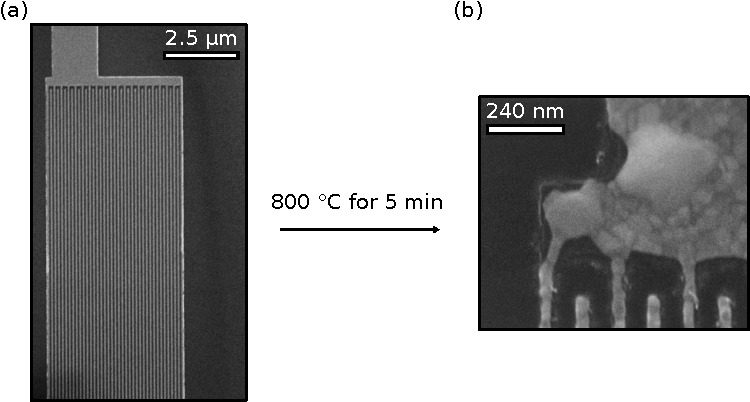
\includegraphics{IDT damaged.pdf}
    \caption{IDTs with $\lambda = \SI{240}{\nano\meter}$ before (a) and after (b) an \SI{800}{\celsius} bake for 5 minutes. These test IDT structures were fabricated by UCSB nanofab.} 
    \label{IDT damaged}
\end{figure}

To fulfil the need of interfacing two disparate devices with competing fabrication requirements, the technique of “flip-chip gating” has emerged in recent years \cite{beukman_noninvasive_2015, chu_creation_2018, satzinger_quantum_2018, robertson_non-invasive_2020}. Similar to the “flip-chip packaging” technique used in commercial semiconductor device processing, flip-chip gating involves flipping one chip onto another, while keeping the two chips separated by an air gap. For example, Refs. \cite{chu_creation_2018} and \cite{satzinger_quantum_2018} used flip-chip gating to couple a superconducting qubit to an acoustic resonator, enabling long-lived quantum states of mechanical motion. Flip-chip gating allowed the authors to optimize the design of the acoustic resonator and the qubit separately, greatly improving the coherence time of their acoustic-electromagnetic hybrid quantum systems and enabling new insights into quantum control of macroscale mechanical objects. Thus, flip-chip construction is a promising tool for interfacing SAW devices with quantum materials.

Figure \ref{flip-chip intro figure} shows a possible design for interfacing a CNT with a SAW using flip-chip construction, to create a topologically-protected quantum pump (see Sec.\ \ref{Thouless pump intro chapter} for further discussion on this system). A SAW device fabricated on LiNbO\textsubscript{3} (as in Sec.\ \ref{IDT methods}) would be flipped onto a suspended CNT (as in \cite{senger_universal_2018}). Etched spacers created with deep-reactive ion etching (RIE) would separate the two chips. For this proposed design, the air gap between the SAW chip and CNT is of paramount importance, as most of the energy of a SAW is contained within one SAW wavelength of the surface \cite{wixforth_surface_1989}. However, prior flip-chip designs do not allow for precise measurement of the flip-chip air gap.

Though prior works had success with flip-chip designs, most prior works do not directly measure their flip-chip’s spacing, nor ensure parallel mounting \cite{chu_creation_2018,satzinger_quantum_2018, bennaceur_mechanical_2015}, with one work estimating their air gap using capacitance \cite{beukman_noninvasive_2015}. In this chapter, I present a flip-chip platform that does not rely on external mounting pressure, and allows for characterization of the flip-chip air gap in multiple areas to determine parallel mounting. Instead of springs or tension arms, my design uses hard-cured varnish and etched Si spacers to hold a precise air gap, enabling a more compact flip-chip. I benchmark this platform by building a flip-chip capacitor using photolithography, deep reactive ion etching (RIE), and a homebuilt flip-chip assembly station. I verify the spacing between the two chips with two independent methods — capacitance, and reflectance spectroscopy — and evaluate the feasibility of a flip-chip without external mounting pressure.

\begin{figure}
    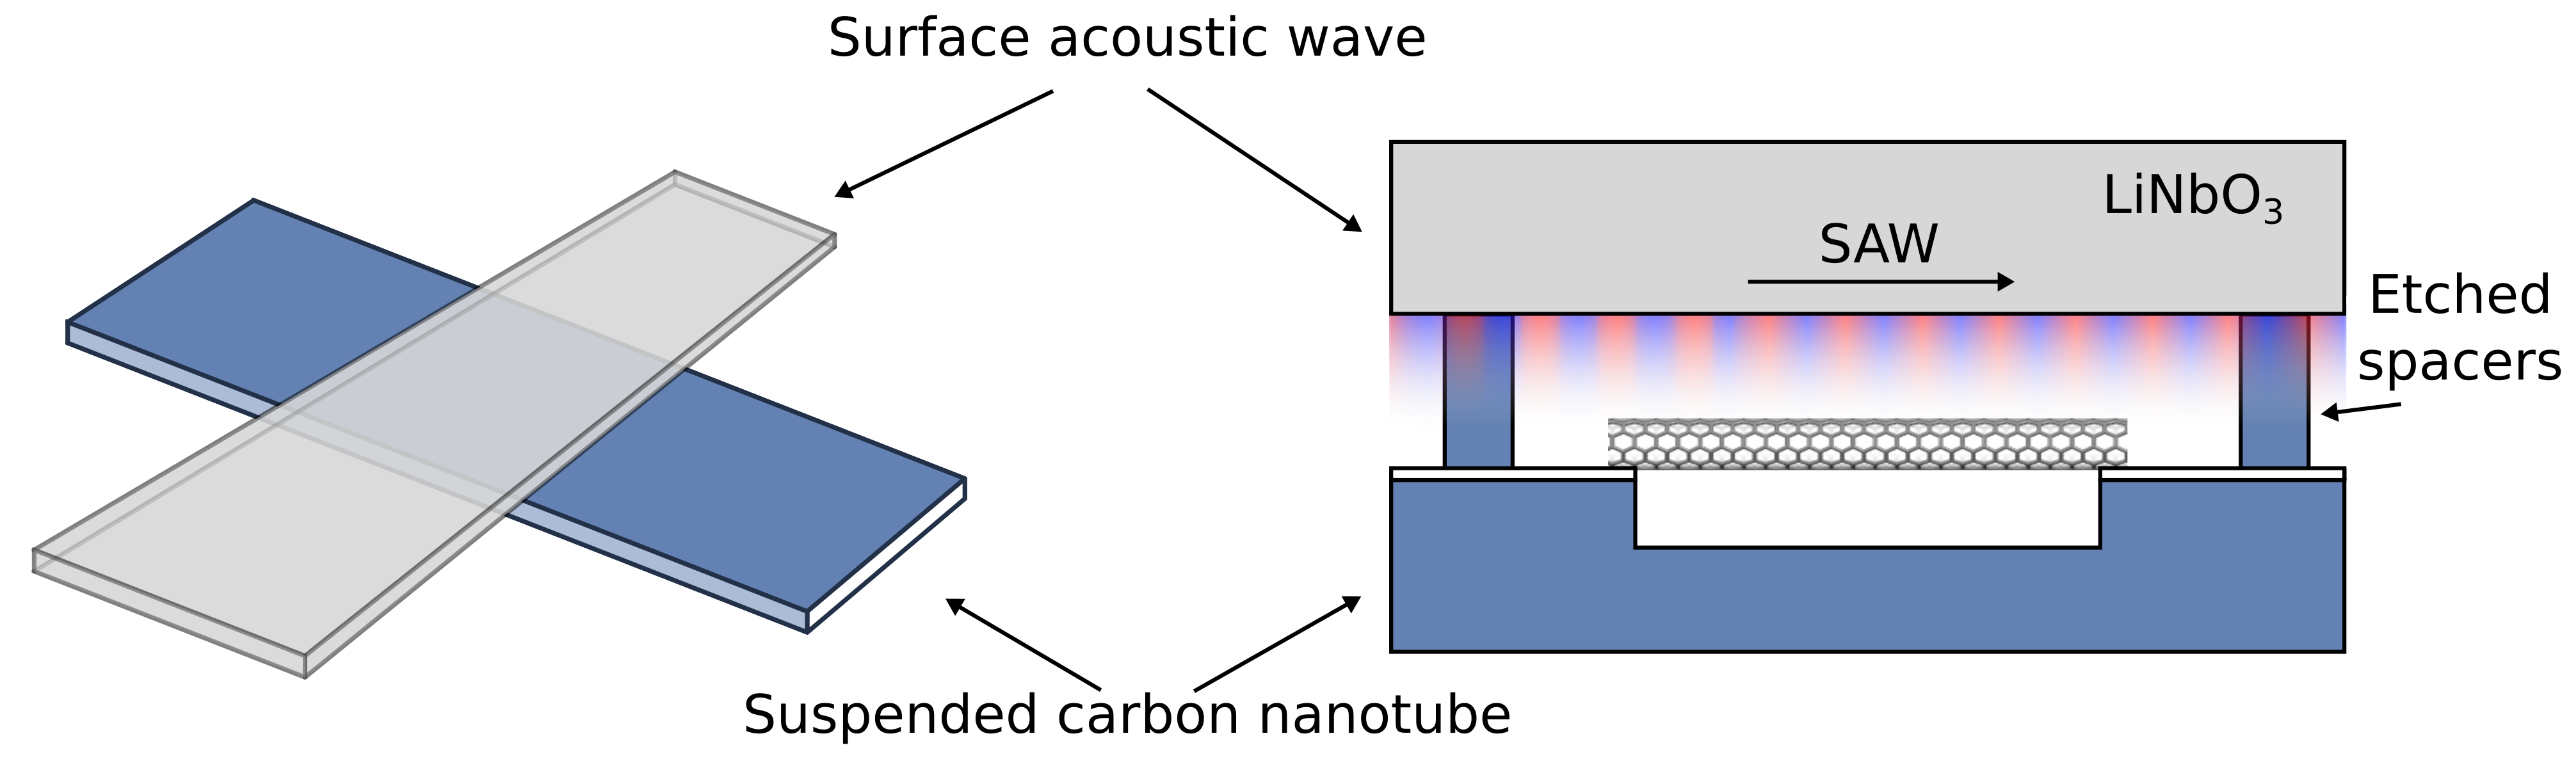
\includegraphics[width=1\textwidth]{Flip-chip intro figure.png}
    \caption{Proposed CNT-SAW flip-chip design, in which a SAW chip and CNT chip are "flipped" onto each other. Etched Si spacers, as described in this chapter, would define the air gap.}
    \label{flip-chip intro figure}
\end{figure}

\section{Measuring flip-chip spacing using interference spectroscopy}

The first method I use to measure the air gap between two chips is interference spectroscopy. Using a laser with a spot size $<$ \SI{1}{\milli\meter}, I can not only measure the central air gap, but probe various spots on the flip-chip to determine if the two chips are parallel. Figure \ref{InterfSpec} shows the optical setup used in the interference spectroscopy measurement.


\begin{figure}
    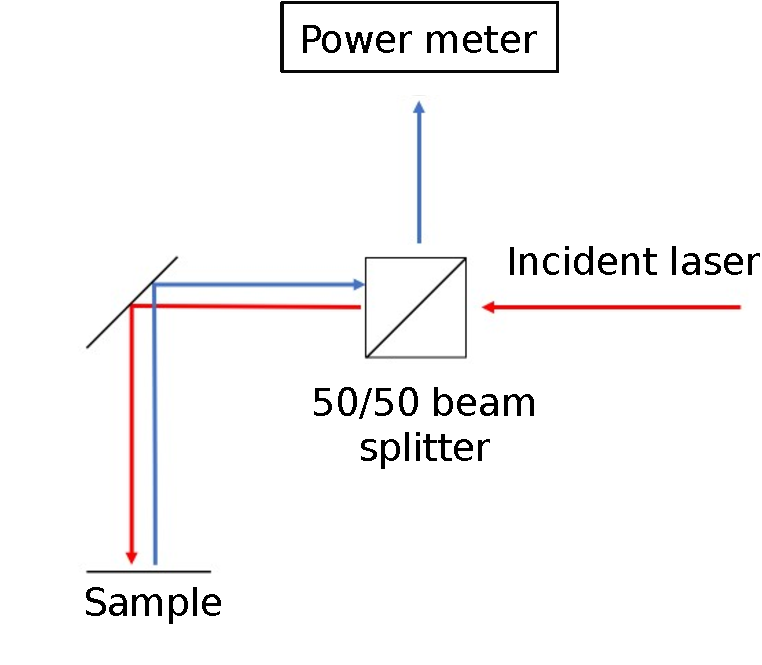
\includegraphics[width = 0.5\textwidth]{Interference spectroscopy.pdf}
    \caption{The interferometer setup used to measure the reflectance of a sample. Incident wavelength is scanned using a Labview-controlled monochromator and plotted against measured reflected power. The colors indicate incident light (red) and reflected light (blue).}
    \label{InterfSpec}
\end{figure}
To correct the reflectance spectrum for wavelength-dependent power fluctuations and substrate effects, I measure a reference spectrum using a bare Si substrate, then subtract this reference spectrum from the measured interference spectrum. Then, I determine the flip-chip air gap by hand-fitting to a model spectrum calculated with Filmetrics’s online thin-film modelling calculator. 

As a first test, I spun a PMMA 495 A11 solution on a Si chip at 2500 RPM for 60 seconds. According to the manufacturer's spin curves, the PMMA layer should be $\approx \SI{1000}{\nano\meter}$ thick. Then, I used the process described in \ref{FCfab} to glue a quartz chip on top to create the Si-PMMA-quartz stack shown in the inset of Fig.\ \ref{PMMAqzspec}. Figure \ref{PMMAqzspec} shows the corrected reflectance spectrum of this Si-PMMA-quartz stack versus the reflectance calculated with the Filmetrics model.


\begin{figure}
    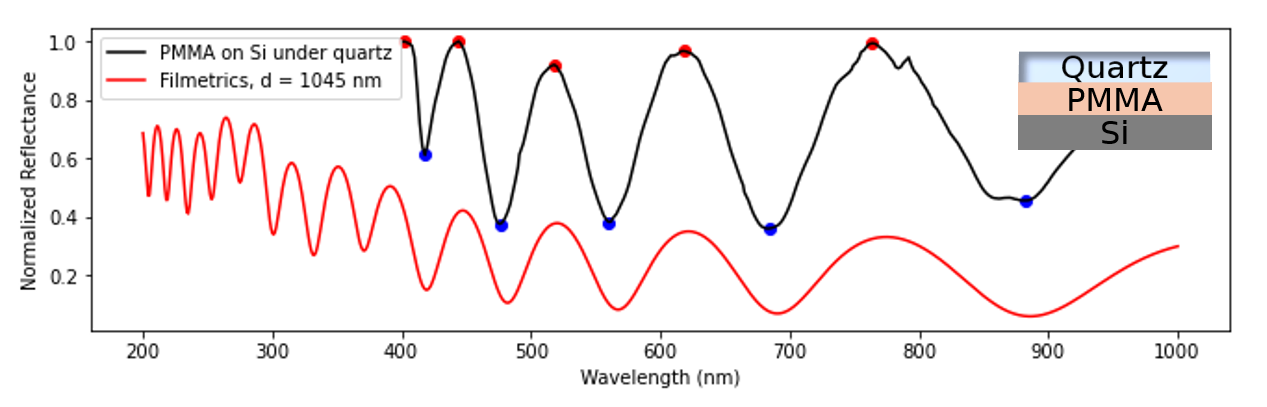
\includegraphics[width=1\textwidth]{qzPMMAsi stack spec.PNG}
    \caption{Corrected measured reflectance of a Si-PMMA-quartz stack compared to the Filmetrics reflectance calculation with \SI{1045}{\nano\meter}-thick PMMA.}
    \label{PMMAqzspec}
\end{figure}
The peaks and troughs of the measured reflectance spectrum are consistent with a PMMA thickness of \SI{1045}{\nano\meter}, close to the predicted spun PMMA thickness, which varifies the validity of this method.

\section{Flip-chip fabrication process} \label{FCfab}
Figure \ref{flip-chip diagram} (a) shows a diagram of my homebuilt flip-chip assembly station. I designed the holder arm with a "tuning fork" structure (Fig.\ \ref{flip-chip diagram} (b)) which allows me to look through the quartz chip to align structures on the top and bottom chips. The tuning fork arm opening is \SI{7}{\milli\meter}, which matches the length of the short side of the bottom chip. This ensures that pressure is applied above the edges of the bottom chip, preventing the quartz chip from bowing outward. 

For all the flip-chips described in this chapter, I used the following assembly process: To create the top and bottom chips, I coated fused quartz and bare p-doped Si wafers (University Wafer) with S1813 photoresist to protect them during the dicing process, then diced the Si into \SI{7}{\milli\meter} $\times$ \SI{12}{\milli\meter} rectangles and the quartz into \SI{4.5}{\milli\meter} $\times$ \SI{12}{\milli\meter} rectangles using a DISCO DAD 3220 wafer dicing saw. Immediately prior to gluing the chips together, I removed the photoresist by soaking in a \SI{60}{\celsius} Remover PG bath for 15 minutes, followed by spraying with acetone and isopropyl alcohol and drying with dry N\textsubscript{2}. Then, I cleaned both chips by submerging them in acetone and rubbing for 20 seconds with a Rubystick T-21 swab to remove any dust \cite{lane_integrating_2021}. Next, using PDMS strips, (Gel-Pak), I mounted them to the homebuilt flip-chip mounting station as shown in Fig.\ \ref{flip-chip diagram} (b). 

\begin{figure}
    \includegraphics{Flip-chip diagram.pdf}
    \caption{(a) A diagram of the homebuilt flip-chip assembly station. (b) Quartz chip mounted to the "tuning fork" arm with gel-pak strips (scale bar = \SI{12}{\milli\meter}). (c) A photograph (scale bar = \SI{12}{\milli\meter}) and (d) optical microscope image (scale bar = \SI{350}{\micro\meter}) of a flip-chip during alignment.}
    \label{flip-chip diagram}
\end{figure}

Figure \ref{flip-chip diagram} (c) shows a photograph of a flip-chip during alignment, and Fig.\ \ref{flip-chip diagram} (d) shows an optical microscope image of the same. First, I rotate the edges of the top and bottom chip to ensure they are perpendicular. Then, I slowly lower the z-stage to bring the chips into contact, watching for interference fringes. As the flip-chip spacing becomes smaller, the interference fringes change. Once the top chip contacts the bottom chip, the spacing will not change as I lower the z-stage, so the interference fringes will remain static. This is how I determine that the two chips are in contact. Once the top and bottom chips are in contact, I glue the two chips together by putting two small beads of GE 7031 varnish at the edges. I hard-cure the varnish using a heat gun at 200 C for 5 minutes, holding the heat gun 20 cm from the chip. I also attempted to use photoresist to glue the chips together, as in Ref.\ \cite{beukman_noninvasive_2015}, but it was difficult to avoid photoresist flowing between the sandwich due to the capillary effect (see Appx.\ \ref{additional flip-chip tests}).

As a first check, a flip-chip's cleanliness can be assessed by viewing the interference fringes (Newton's rings) visible through its quartz top. Figure \ref{newtonsrings} illustrates the pattern of interference fringes expected from different surface topographies. If the two surfaces are parallel, the interference fringes will form parallel bands (Fig.\ \ref{newtonsrings} (A)). Conversely, if a large piece of dust comes between the two surfaces, a point with many small concentric fringes will be visible, encircling the dust particle (Fig.\ \ref{newtonsrings} (B)). This method was used in \cite{bennaceur_mechanical_2015} to confirm that no large dust particles settled between the two sides of their flip-chip.

%TODO: Caption and fix ref
\begin{figure}
    \includegraphics[width=1\textwidth]{newtonsrings.png}
    \caption{Interference patterns formed by a flat surface in contact with (A) A flat surface, (B-C) Convex surface with contact point indicated by $X$, and (D) Irregular surface with contact points $X_1$ and $X_2$.  From \cite{noauthor_newtons_nodate}.}
    \label{newtonsrings}
\end{figure}



\subsection{Smallest achievable air gap} \label{smallest achievable air gap}
Before attempting to control the air gap between two chips, I first need to determine the smallest air gap that I can achieve between two clean chips with no spacers between them. Figure \ref{interference sandwich} (a) shows a flip-chip constructed from pristine quartz and Si chips using the method described in Sec.\ \ref{FCfab}. I performed three interference spectroscopy measurements on this chip with no spacers — one in the center, and one on each edge — to determine if the chips are mounted parallel to each other.


\begin{figure}
    \includegraphics[width=1\textwidth]{interference sandwich image and spectrum.pdf}
    \caption{(a) A flip-chip with no spacers made from quartz and Si. The three circles indicate the spots at which I directed the laser for interference spectroscopy air gap measurement. (b) The reflectance spectrum from the central spot compared to the Filmetrics model with a \SI{3.2}{\micro\meter} air gap.}
    \label{interference sandwich}
\end{figure}

The air gap measurement confirms that the air gap on one side of the flip-chip is $\approx \SI{1}{\micro\meter}$ larger than the air gap on the other side. I constructed two other flip-chips with no spacers, and the smallest spacing I could achieve was the \SI{2.4}{\micro\meter} side of the flip-chip shown in Fig.\ \ref{interference sandwich}. When I observed visible dust between the chips, I uncoupled the flip-chip and cleaned the Si and quartz chips. No visible dust is present between the flip-chip shown in Fig.\ \ref{interference sandwich}. However, unseen dust of size $\approx \SI{2.4}{\micro\meter}$ could be present, as the flip-chips described in this chapter were not fabricated in a clean room. The air gap limit could also arise from thickness variation over the surface of the quartz and Si wafers. Ref.\ \cite{bennaceur_mechanical_2015} attributes their minimum achievable flip-chip spacing (fabricated in a class-100 clean room) of 50 to \SI{200}{\nano\meter} to the top and bottom chips not being perfectly flat across the contact area. We did not buy special $< \SI{1}{\micro\meter}$ total thickness variation Si wafers from University Wafer; furthermore, they do not quote the thickness variation of their fused quartz wafers. From these flip-chips with no spacers, I determine \SI{2.4}{\micro\meter} to be the lower bound for the air gap that I can reasonably achieve with etched Si spacers, and use this to inform my flip-chip design in the next section.


\section{Flip-chip capacitor with deep reactive ion-etched silicon spacers} \label{FC SIspacer}
In the previous section, I determined that the smallest spacing that I can reasonably achieve between two pristine chips is \SI{2.4}{\micro\meter}. However, this does not exclude the possibility of achieving a tighter air gap in a small area of the flip-chip while leaving most of the flip-chip spaced by $\geq$ \SI{2.4}{\micro\meter}. A two-tier etch has previously been used to achieve a narrow central spacing of $<$ \SI{1}{\micro\meter} while leaving a larger air gap between most of the area of the flip-chip \cite{beukman_noninvasive_2015}. This reduces the likelihood of dust becoming sandwiched in-between the chips and preventing close spacing. 

Figure \ref{twotier} shows the two-tier deep reactive ion etch (RIE) process that I use to create pillars that define the flip-chip spacing. I first print 50 $\times$ \SI{50}{\micro\meter} Cr squares with center spacing \SI{360}{\micro\meter} and thickness \SI{150}{\nano\meter} on a p-doped Si substrate using photolithography (Fig.\ \ref{twotier} (a) (1)). This Cr serves as an etch mask for the deep RIE. Then, I use the SI etch recipe described in \ref{Si RIE recipe} and an Oxford Plasmalab 100 plasma etch system to etch \SI{460}{\nano\meter} into the Si (Fig.\ \ref{twotier} (a) (2)). This first etch defines the center spacing of the flip-chip. Next, I print the capacitor structure using photolithography and metallization of \SI{150}{\nano\meter} Cr, consisting of a 750 $\times$ \SI{750}{\micro\meter} square center pad and \SI{50}{\micro\meter} wires that extend to the edges of the chip (Fig. \ref{twotier} (a) (3)). I fabricated this same capacitor structure on both the Si and quartz chips (Fig.\ \ref{twotier} (b)). The long wires allow me to make electrical contact to the central pad of the capacitor when the two chips are sandwiched together Then, I etched the final \SI{5}{\micro\meter} into the Si (Fig.\ \ref{twotier} (a) (4)). For both Si etches, I determined the exact etch depth using AFM. I assembled the flip-chip capacitor using the process described in Sec.\ \ref{FCfab}. 
 

% \begin{figure}
%     \includegraphics[width = 0.5\textwidth]{FCCap during alignment.pdf}
%     \caption{View through the microscope camera during initial alignment of the flip-chip capacitor (the top and bottom chips are still far from each other, so no Newton's rings are visible).}
%     \label{FCcap during alignment}
% \end{figure}

%TODO: fix text sizes on this one and size of image
\begin{figure}
    \includegraphics[width=1\textwidth]{Two-tier etch.pdf}
    \caption{(a) Two-tier etch process for defining the center gap and post height of the flip-chip. The denoted measurements are estimated from known Cr deposition rates and known Cr and Si etch rates (see Appendix \ref{Si RIE recipe}). (b) The completed top and bottom sides of the flip-chip capacitor, before assembly.}
    \label{twotier}
\end{figure}

Figure \ref{FCCap Ref Summ} (a) shows the measured reflectance spectra for the left and right side of the flip-chip capacitor. The left side best-matches \SI{5.00(5)}{\micro\meter}, while the right side best-matches \SI{6.50(5)}{\micro\meter}. The error denotes the smallest step for which the best hand-fit was obvious. For example, during the fitting process, it was clear that, for the left side, \SI{5.00}{\micro\meter} was a better fit than \SI{4.95}{\micro\meter} or \SI{5.05}{\micro\meter}. Figure \ref{FCCap Ref Summ} (b) shows the schematic of the completed flip-chip capacitor.

\begin{figure}
    \includegraphics[width = 1\textwidth]{Flip-chip capacitor reflectance summary.pdf}
    \caption{(a) Reflectance spectrum versus Filmetrics model for the left (left) and right (right) sides of the flip-chip capacitor. From these spectra, I determined the air gap to be \SI{5.00(5)}{\micro\meter} on the left side, and \SI{6.50(5)}{\micro\meter} on the right side. (b) Schematic of the flip-chip capacitor. AFM measurements of the chip geometry are indicated near the center of the schematic.}
    \label{FCCap Ref Summ}
\end{figure}

AFM measurements of the Cr thickness (\SI{48}{\nano\meter}), central mesa (\SI{4.37}{\micro\meter}), and spacers (\SI{4.98}{\micro\meter}) are indicated on the diagram.

\begin{table}
    \centering
    \begin{tabular}{|c|c|}
        \hline
        Cr metal on top chip & \SI{48(1)}{\nano\meter} \\
        \hline
        Etched spacers & \SI{4.980(5)}{\micro\meter} \\
        \hline
        Central mesa & \SI{4.370(5)}{\micro\meter} \\
        \hline
        \hline
        Designed center gap & \SI{0.563(10)}{\micro\meter} \\
        \hline
    \end{tabular}
    \caption{AFM measurements of the chip geometry. The designed center gap is derived from the height difference between the etched spacers and central mesa, and the thickness of the evaporated metal on the top quartz chip.}
    \label{flip-chip AFM table}
\end{table}

Figure \ref{FCCap Ref Summ} illustrates that I did not achieve parallel mounting. The left air gap agrees precisely with the etched post height of \SI{4.950(5)}{\micro\meter}; however, the right air gap sits \SI{1.50(5)}{\micro\meter} taller. The designed center gap is \SI{0.563(5)}{\micro\meter}, from AFM measurements of the posts and central mesa (Table \ref{flip-chip AFM table}). Therefore, I estimate my flip-chip capacitor spacing to be \SI{1.313(55)}{\micro\meter} (\SI{0.563(5)}{\micro\meter} + \SI{1.50(5)}{\micro\meter}/2). Though I did not achieve parallel mounting, this emphasizes the strength of determining the air gap with optical methods. Before mounting the chip, wire bonding, and taking electrical measurements, the air gap of a flip-chip can be estimated, and parallel mounting can be verified. If the estimated air gap is not suitable, or the top and bottom chips are not parallel, the flip-chip can be deconstructed, cleaned, and re-mounted (7031 varnish readily dissolves in a solution of 99\% ethanol). Then, once a suitable estimated air gap is achieved, a more precise air gap measurement can be made using capacitance.


\section{Flip-chip air gap measurement with capacitance}
The total impedance of my flip-chip capacitor is the sum of the capacitor impedance and series resistance
\begin{equation}
    Z = R_s + Z_C = R_s + \frac{1}{i\omega C}.
\end{equation}
Assume an AC signal $V = V_0 \mathrm{exp}(i\omega t)$ is applied to the flip-chip. Then, the AC current $I$ through the capacitor is 

\begin{equation} \label{current full}
    I = \frac{V}{Z} = \frac{V}{R_s + 1/i\omega C.} = V \frac{i\omega C}{1 + i\omega C R}\approx V i\omega C (1 - i\omega C R) = V(R C^2 \omega ^2 + i\omega C),
\end{equation}
where $C = \epsilon_0 A / d$ is the capacitance of the flip-chip, and I assume that the resistance is small, so $\omega C R \ll 1$. The measured current is then the real part of Eq.\ \ref{current full}, 

\begin{equation}
    I = V_0\omega^2 R C \mathrm{cos}(\omega t) + V_0 C \omega \mathrm{sin}(\omega t).
\end{equation}
Therefore, by applying an AC signal to the flip-chip capacitor and measuring the sine component of the resultant current, the distance between the flip-chip capacitor plates can be determined using $d = 2\pi f \epsilon_0 A V_0 / I$. 

Figure \ref{flipping chips} shows a schematic and photograph of the completed flip-chip capacitor, and Fig. \ref{FC cap measurement} (a) shows the experimental setup that I use to measure its capacitance of my flip-chip. I use a Stanford SR830 lock-in amplifier to apply an AC signal of $V_0 = $ \SI{100}{\milli\volt} at $f = $ \SI{200}{\hertz} and measure the sine component of the resultant current. 

\begin{figure}
    \includegraphics[width=0.5\textwidth]{flipping chips.pdf}
    \caption{(a) Schematic of the completed flip-chip capacitor. (b) Optical image of the completed flip-chip capacitor. Wires are seen soldered to the silver paint, making electrical contact to the top and bottom chips.}
    \label{flipping chips}
\end{figure}

\begin{figure}
    \includegraphics[width = 0.5\textwidth]{FC capacitance measurement.pdf}
    \caption{(a) schematic of the capacitance measurement. (b) Dependence of central air gap modulation with respect to location of applied mounting pressure. The edge force was applied onto the quartz chip, above the etched spacers closest to the edge of the Si chip. The central force was applied directly above the capacitor pads.}
    \label{FC cap measurement}
\end{figure}



Figure \ref{FC cap measurement} shows the results of the capacitance central air gap measurement. To determine the effect of mounting pressure, I measured the capacitance in three scenarios: applying no force, applying force on either edge of the flip-chip, and applying force in the center of the flip-chip (directly on the capacitor plates). With no mounting pressure, I determined the central air gap to be \SI{1.33(1)}{\micro\meter}, which is in very good agreement with the estimated central air gap from reflectance spectroscopy of \SI{1.36(6)}{\micro\meter} determined in Sec.\ \ref{FC SIspacer}. When applying edge force to simulate mechanical mounting pressure, the air gap closed to  \SI{0.688(10)}{\micro\meter}, which is close to the designed air gap defined by the etched posts (measured with AFM to be \SI{0.563(10)}{\micro\meter}). Applying a strong enough central force short-circuits the capacitor plates. 

Figure \ref{quartz bending} shows the geometry of the bent quartz chip when applying a central force to the flip-chip capacitor, short-circuiting the top and bottom chips. The bend is greatly exaggerated. Assuming that the quartz chip bends directly at the Si posts, it bends by \SI{0.563(10)}{\micro\meter} over \SI{1}{\milli\meter}, corresponding to a bending radius of \SI{0.22}{\meter} (assuming the bend forms an arc). Therefore, the strain in the quartz is \SI{0.85}{\nano\meter} / \SI{1}{\milli\meter} = $8.5 \times 10^{-5} \% $.


\begin{figure}
    \includegraphics[width = 0.75\textwidth]{quartz bending.pdf}
    \caption{Geometry of the bent quartz chip with a centrally-applied force that short-circuits the top and bottom capacitor pads.}
    \label{quartz bending}
\end{figure}


\section{Conclusion}
In this section, I built a flip-chip capacitor by sandwiching patterned quartz and etched Si chips together with hard-cured varnish. I used two independent methods to characterize the gap between the two chips — interference spectroscopy (which I refer to as the "optical method") and capacitance. Combining both methods allows for a complete characterization of the flip-chip air gap at multiple locations, and a precise measurement between the gate chip and quantum material to be gated. The optical air gap measurement is useful for quick determination of the air gap before spending time wire bonding the chip and mounting it in a cryostat. Measuring the flip-chip air gap using interference spectroscopy is a novel method — prior reports of flip-chip devices did not use optical methods to measure their flip-chip spacing \cite{beukman_noninvasive_2015, chu_creation_2018,satzinger_quantum_2018,bennaceur_mechanical_2015}. Using this optical method, I found that I was not able to achieve parallel mounting without external mounting pressure. This is likely due to the arm of my homebuilt assembly station not being perfectly level, leading to uneven mounting pressure. This is in agreement with the Si-quartz sandwiches that I created without patterned spacers (Sec.\ \ref{smallest achievable air gap}), in which I noticed that one side was always $\approx \SI{1}{\micro\meter}$ higher than the other, as measured using interference spectroscopy. Conversely to the optical method, the capacitance air gap measurement requires electrical contact to the chip, but can measure the air gap more precisely. The central spacing that I measured with capacitance (Fig.\ \ref{FC cap measurement}) in the cases of no mounting pressure and edge mounting pressure are in good agreement with the flip-chip geometry determined by AFM and optical measurement (Fig.\ \ref{FCCap Ref Summ}). When I applied mounting pressure to the central capacitor pads, I was able to bend the quartz chip by \SI{0.563(10)}{\micro\meter} and short-circuit the capacitor pads. This suggests the possibility of measuring the air gap of a flip-chip inside a cryostat and tuning the air gap in-situ. Future flip-chip devices which interface a CNT with a SAW could be designed with a capacitive pad in multiple locations on top and bottom chips. Then, A motorized stage inside the cryostat, such as in \cite{inbar_quantum_2023}, could be used to apply mounting pressure to the flip-chip while measuring the capacitor array to minimize the air gap and maximize the strength of coupling between the SAW gate and CNT. 


\chapter{Conclusions} \label{conclusions chapter}

\section{Summary}
In this dissertation, I explore methods for interfacing 2D and 1D quantum materials with surface acoustic waves (SAWs). Chapter \ref{methods chapter} Sections \ref{fabricating 2D devices} through \ref{AFM cleaning main section} describe the methods that I use to make 2D devices. I outline the tricks that I have learned for exfoliating graphene and h-BN. Then, I describe the hot pickup technique for stacking 2D materials in detail, putting particular emphasis on how the viscoelastic stamps are constructed. I continue by describing a method of using a highly-adhesive polymer to remove unwanted 2D flakes from the surface. This is particularly important for interfacing 2D materials with SAWs, as a SAW device can be rendered inoperable by unwanted graphene flakes shorting its interdigitated electrodes. I finish my discussion on 2D devices by describing how I fabricate metal contacts and clean them with contact-mode AFM before transferring a 2D heterostructure onto them. Finally, Chapter \ref{methods chapter} ends with a discussion on fabricating SAW devices (Sec.\ \ref{IDT methods}), in which I outline design rules for fabricating SAW devices and methods for measuring their frequency response to verify their performance.

In Chapter \ref{AE charge pumping paper}, we report the first measurements of charge pumping in h-BN-encapsulated graphene in literature. I fabricated two top-gated graphene devices for this study: One which is fully encapsulated in h-BN, and one which is capped with h-BN but sits directly on the LiNbO\textsubscript{3} substrate. The LiNbO\textsubscript{3} induces electrostatic disorder in the half-encapsulated device, allowing us to study the effect of disorder on the acoustoelectric signal. In prior studies of charge pumping in lower-quality graphene samples, authors noted qualitative discrepancies between their experimental data and the single-carrier classical relaxation model (I describe the single-carrier classical relaxation model in Sec.\ \ref{classical relaxtion model}). We extend this classical relaxation model to describe mixed-carrier transport near the charge neutrality point (the region in which both electrons and holes are present — see Sec.\ \ref{AE paper discussion}). The mixed-carrier model is an excellent fit to our experimental data for both devices. The quantitative framework outlined in this study will assist future SAW-based probes of quantum phenomena in graphene and other 2D materials.

In Chapter \ref{flip-chip chapter}, I introduce a novel design for interfacing pristine quantum materials with SAWs using a flip-chip construction. Using a homebuilt flip-chip assembly station, I achieve a gap of \SI{0.688(10)}{\micro\meter} between sandwiched quartz and Si layers without external mounting hardware to apply pressure to the flip-chip. This design improves on previous flip-chip designs by allowing precise measurement of the air gap between the top and bottom sides of the flip-chip using two independent methods. The first method is reflectance spectroscopy, which I use to measure the air gap and assess the parallelism of the two chips prior to making electrical contact. This optical method is complemented by a capacitance method, which offers more precise measurement of the air gap and can be used while the flip-chip is mounted in a cryostat to verify the air gap at cryogenic temperatures. While further work is required to ensure even mounting force and improve the parallelism of the mounting, this flip-chip design could be used in future studies into SAW-gated quantum materials. For instance, suspended carbon nanotubes and SAW devices present competing fabrication requirements. This flip-chip design could be used to non-invasively couple SAWs to a pristine suspended carbon nanotube, in pursuit of topologically-protected charge pumping.





\section{Outlook and future work} \label{outlook and future work}
The results on acoustoelectric charge pumping in encapsulated graphene presented in Ch.\ \ref{AE charge pumping paper} give credence to future works seeking to probe and control phenomena in low-dimensional quantum materials. SAWs are a welcome, if currently underutilized addition to the toolbox of techniques which are currently used to tune the properties of 2D materials (static electric field, magnetic field, pressure, and strain). For example, interactions between SAWs and moiré heterostructures are scantly explored, but represent a particularly interesting direction for future work. 

Moiré heterostructures exhibit countless exotic states of matter which have proven to be widely tunable with current techniques. However, SAWs are a promising new tool for probing and controlling phenomena in moiré heterostructures. The periodicity of many moiré superlattices is on the order of achievable SAW wavelengths. This congruence begs for future studies exploring on SAW-driven tuning of quantum phenomena in moiré heterostructures. Furthermore, SAWs present the possibility of creating dynamic, tunable superlattices in 2D materials. Interest in engineered 2D superlattices has exploded in recent years, since the discovery of unconventional superconductivity in twisted bilayer graphene \cite{cao_unconventional_2018}. By tuning the twist angle between two sheets of graphene (and thus the periodicity of the moiré superlattice), bilayer graphene can not only exhibit superconductivity, but also correlation-induced insulating states, magnetism, quantized anomalous Hall states, and many more exotic phenomena \cite{andrei_graphene_2020}. In 2D semiconductors, which exhibit exciton dynamics that are of great interest for next-generation electronics, tuning the moiré superlattice provides more control over the spin and valley degrees of freedom \cite{ciarrocchi_excitonic_2022}. SAWs could be used similarly to tune the properties of moiré materials. 

Another promising direction for future work is contactless probing of 2D materials using SAWs. One work demonstrated SAW-based probing of quantum oscillations in graphene \cite{fang_quantum_2023}. However, the same technique could be a powerful tool for probing 2D semiconductors. Contactless probing using SAWs could circumvent the challenges of making quality electrical contact to 2D semiconductors for conventional transport measurements \cite{miao_recent_2022}. 

Of particular interest for controlling quantum phenomena in low-dimensional materials is the nonlinear charge pumping regime which we observed in graphene (Sec.\ \ref{nonlinear acoustoelectric effect}). In the nonlinear charge pumping regime, charge carriers are completely trapped in the SAW potential and flow as stripes moving at the speed of sound. Though more work is needed to understand the differences between nonlinear charge pumping in graphene and prior observations of the effect in GaAs/AlGaAs heterostructures, the ability to completely trap charge carriers in potential wells would be a powerful tool with which theoretical SAW-based quantum phenomena could be realized. For example, theoretical works have proposed that SAW-driven pumping could be used in 2D materials to pump heat without charge transfer \cite{andreev_electronic_2022}, or in a 1D system to transport spin-entangled electrons for quantum information applications \cite{giavaras_quantum_2006}. Charge pumping in the nonlinear regime is an exciting possiblity for experimentally realizing these theoretical designs.

SAW-based charge pumping is also a path to realizing novel topological phenomena in 2D materials. For example, the nontrivial topology of the $K$ and $K'$ valleys in MoS\textsubscript{2} is predicted to cause $K$ and $K'$ electrons to drift in opposite directions when pumped by a SAW (the "valley acoustoelectric effect") \cite{kalameitsev_valley_2019}. Such independent control over $K$ and $K'$ electrons would be a valuable tool for valleytronics devices.

Finally, using the methods presented in this dissertation, SAWs could be used to adiabatically pump charge through an encapsulated (or suspended) carbon nanotube, realizing a practical integer charge Thouless pump to help define a better standard for current \cite{pekola_single-electron_2013,scherer_singleelectron_2019}; or, to investigate fractional topological charge pumping arising from strongly-interacting  \cite{novikov_devils_2005}. Complete trapping of charge carriers in the periodic potential wells is a central requirement of Thouless's prediction. Thus, either using the flip-chip design presented in Ch.\ \ref{flip-chip chapter} to minimize the gap between a SAW and suspended nanotube and maximize the height of the periodic potential, or utilizing an h-BN-encapsulated nanotube which sits only tens of nanometers from the SAW, are both promising paths towards achieving topological charge pumping in carbon nanotubes.


\pagebreak

\bibliography{thesis}
\bibliographystyle{unsrturl}

\pagebreak

\appendix
\chapter{Fabrication recipes}

\section{Photolithography recipe} \label{photolithography recipe}

\begin{enumerate}
    \item Cleanly pipette enough LOR 3A photoresist to cover the substrate. Spin at 4000 RPM for 45 seconds.
    \item Bake at 180 C for 4 minutes
    \item Cleanly pipette enough S1813 photoresist to cover the substrate. Spin at 4000 RPM for 30 seconds.
    \item Bake at 120 C for 2 minutes
    \item Edge bead removal: The edges of the chip will have built-up photoresist that is many times thicker than the rest of the chip. Edge bead removal is particularly important for fine features on small substrates, as edge beads prevent the chip from fully contacting the mask. Try putting a tiny amount of Remover PG on the tip of a clean swab, such as a small square of cleanroom wipe, then swab your edges at a 45-degree angle to remove edge beads. 
    \item Expose chip for 12 seconds at \SI{6}{\milli\joule/\centi\meter^2}.
    \item Develop for 100 seconds in AZ-300 MIF developer
    \item Rinse with DI water and blow dry with N\textsubscript{2}.
\end{enumerate}

\section{Si reactive ion etch (RIE) recipe}\label{Si RIE recipe}

\begin{itemize}
    \item SF\textsubscript{6}: 14.0 sccm
    \item CHF\textsubscript{3}: 35.0 sccm
    \item 100 W RF power
    \item Chamber pressure = 10 torr
    \item Si Etch rate: \SI{40}{\nano\meter/\minute}
    \item Cr etch rate: \SI{0.8}{\nano\meter/\minute}

\end{itemize}


\section{Calibrating applied force with MFP-3D AFM} \label{force curve appendix}

The following began as an excerpt from the Minot Lab wiki. I later updated it for the modern version of the MFP-3D software.

Static force curves allow you make graphs of deflection versus tip height for single pushes onto a sample. There is a calibration process that is necessary to make these measurements accurate.

Start with the tip far away from the surface to measure virtual deflection. If you don't, the tip will crash into the surface because the trigger channel is set to “none” by default. Calibrating the measured deflection is a two part process: First, with the Trigger Channel left at "none" and all other options left at their default values, press the Single Force button near the bottom of the Master Panel. A new window should open with a noisy red and blue graph that looks linear. This line is the virtual deflection. In the "Cal" tab open the "Set Sens." dropdown list and click on "Virtual Defl Line". A black line will appear on the force vs displacement graph. The program automatically records these fit parameters in the virtual deflection box in the "Cal" tab. Virtual deflection is now calibrated.\footnote{"Virtual deflection" is a change in deflection as a function of height which is due to tiny changes in the optical path of the laser throughout the Z range. Virtual deflection should not be confused with "squeeze-film damping", which is a reduction in free-air amplitude as the tip is lowered toward a surface. Squeeze-film damping arises due to air that becomes "trapped" between the cantilever and the sample, thereby applying extra forces to the cantilever as it oscillates. Squeeze-film damping is observed only in the close vicinity of a sample, whereas virtual deflection can be observed in the absence of a sample.}
        
Next, you will engage the surface with the tip. In this step, you will calibrate the Deflection InvOLS, or Inverse Optical Lever Sensitivity. It is the sensitivity of the detector-cantilever combination, which lets you relate deflection to an actual force value. It's the inverse because the bigger the number, the less sensitive the detector is. 

In the Trigger Channel dropdown list choose "Deflection" and set the trigger point to \SI{20}{\nano\meter}. Press "Single Force". The first graph you see will have a lot of extraneous data as the tip finds the surface. After the tip has reached the deflection trigger point, it will disengage and retract a small distance from the surface. A clean tip should produce a deflection curve that looks like a backwards checkmark. The red and blue (engage/retract) lines should lie very near to one another. Figure \ref{force curve} shows a force curve for a dirty tip, where the engage/retract lines do not overlap.

\begin{figure}
    \includegraphics{force curve.pdf}
    \caption{A force curve for a dirty AFM tip, in which the engage and retract curves are wildly different. The colors indicate engaging (red) and retracting (blue) the AFM tip.}
    \label{force curve}
\end{figure}

Next, with the graph window selected, press CTRL+I to bring up the cursors. Place the cursors (circle and square objects that pop up at the bottom of the window) on the left part of the graph where the tip is pressing against the surface, selecting a representative portion of the line. (The line of interest is the far left linear line with a negative slope) Make sure the cursors are on the same line. Do this by pressing the left/right arrow keys. If the cursors are on the same line they will move in the same direction.

Select "Deflection InvOLS" from the "Set Sens." dropdown list. The program automatically records the offset in the “Defl InvOLS” box. Click "Withdraw". You are now done calibrating the Deflection.
   
To measure the AFM tip's spring constant: First, set the deflection to zero using the left-side thumb wheel on the AFM head. Click the Thermal button on the right side of the Master Panel and click the Capture button at the top left of the Thermal Graph window. This will bring up the thermal graph. Allow it to collect at least 100 samples.

There should be a spike in the graph that corresponds to your driving frequency. Ensure that this makes sense from your tuning parameters — lower-frequency peaks can appear as well. Use the mouse to drag a box around this peak and expand it through the right click menu. When the peak is well-defined press "Stop Thermal". Click the Fit button. A blue line will now fit to the peak. If the fit looks good, continue. The Spring Constant of the cantilever is now measured and updated in both the Thermal and Main tabs.

Now you can use the measured spring constant to convert between your desired force and deflection in nm. You can use the Force Curve dialog box to convert between deflection in nm and deflection in volts. This deflection voltage is your desired set point in contact mode.



% \section{Comparison between EBL and photolithography process on LiNbO\textsubscript{3}}
% \begin{itemize}
%     \item \textbf{EBL process for encapsulated graphene FET on LiNbO\textsubscript{3} with edge contacts:}
%     \begin{itemize}
%     \item Transfer encapsulated GR onto substrate
%     \item Spin EBL resist
%     \item Deposit charge dissipation layer (thin Al)
%     \item Exposure (edge contact etch)
%     \item Etch Al
%     \item Develop resist
%     \item RIE etch for edge contacts
%     \item Spin EBL resist
%     \item Deposit Al
%     \item Exposure (contact metal)
%     \item Etch Al
%     \item Deposit S/D contacts
%     \item Spin EBL resist
%     \item Deposit Al
%     \item Exposure (gate contact)
%     \item Etch Al
%     \item Deposit gate contact
%     \end{itemize}
%     \item \textbf{Photolithography process for graphene FET on LiNbO\textsubscript{3}:}
%     \begin{itemize}
%     \item Spin photoresist
%     \item Print S/D contacts
%     \item Deposit S/D contacts
%     \item Transfer encapsulated GR onto substrate
%     \item Spin photoresist
%     \item Print gate contact
%     \end{itemize}
%     \end{itemize}
    





% \chapter{Electron-beam lithography} \label{electron-beam lithography} 
% Electron-beam lithography uses the electron beam of a scanning electron microscope (SEM) to expose a polymer resist in a desired pattern. The electron beam breaks the bonds of the polymer, allowing it to be washed away with a chemical developer. 

\chapter{Additional flip-chip tests} \label{additional flip-chip tests}
I initially tried to use photoresist as spacers for flip-chip construction, following the work of \cite{bennaceur_mechanical_2015}. However, I found that the minimum spacing I could achieve was greater than a single layer of spun S1813 photoresist ($\approx \SI{1500}{\nano\meter})$, so I transitioned to using etched Si spacers. Also, the photoresist tended to flow between the flip-chips due to capillary action, so I found that GE 7031 varnish worked much better as glue. Figure \ref{PRFC} shows my attempts at photoresist-spaced and photoresist-glued flip-chips.


\begin{figure}
    \includegraphics[width = 1\textwidth]{photoresist flip-chips.png}
    \caption{(a) A flip-chip with sandwiched quartz and Si surfaces separated by a grid of \SI{50}{\micro\meter}-wide $\approx \SI{1.4}{\micro\meter}$ S1813 photoresist squares spaced by \SI{350}{\micro\meter}. (b) A flip-chip where the quartz and silicon are separated by $\approx$ \SI{1}{\micro\meter} micron of spin-coated PMMA. Photoresist can be seen to have flowed in-between the flip-chip due to capillary action. (c) The grid of photoresist squares under quartz during alignment. (d) A single \SI{50}{\micro\meter}-wide square.
    }
    \label{PRFC}
\end{figure}

% \chapter{Additional data}

% \section{Additional Surface acoustic wave device data}
% Al vs Au IDTs?

% \chapter{Transferred contacts for high-quality contact to 2D semiconductors}

% \chapter{Gate-tunable photoluminescence in h-BN-encapsulated MoS2}

% \begin{figure}
%     \includegraphics[width=1\textwidth]{PL before-after contact.pdf}
%     \caption{}
% \end{figure}

% \begin{figure}
%     \includegraphics[width=1\textwidth]{First Vg PL sweeps.pdf}
%     \caption{}
% \end{figure}

% \begin{figure}
%     \includegraphics[width=1\textwidth]{Second Vg sweep.pdf}
%     \caption{}
% \end{figure}

% \begin{figure}
%     \includegraphics[width=1\textwidth]{exciton dynamics summary.pdf}
%     \caption{}
% \end{figure}

\chapter{What makes a material "topological"?} \label{appendix on topology}

In this Appendix, I discuss topological phenomena in more detail, giving an overview of the origin of Berry phase and the Chern number. This is additional background to the Thouless pump system discussed in Sec.\ \ref{Thouless pump intro chapter}.

The quantity that underlies topological phenomena in quantum materials is the Berry phase (also known as geometric phase). Michael Berry studied the cyclic, adiabatic evolution of an eigenstate through momentum space and found that, though the beginning and ending state of the system are identical, the state gains a phase difference which depends on its path, but not the rate at which the path is traversed \cite{berry_quantal_1984}. Since then, researchers have realized that the Berry phase of a quantum system drastically affects many of its physical properties \cite{xiao_berry_2010}. The Berry phase gives rise to novel quantum phenomena such as the integer, anomalous, spin, and valley Hall effects, and many more phenomena which have been predicted but not yet realized experimentally, including topological SAW-driven phenomena. 

Here, I summarize the origin of Berry phase under an adiabatic evolution, which is central to the Thouless pump. This discussion follows that of Ch.\ 5 of Ref.\ \cite{sakurai_modern_1985}

The time evolution of a quantum system is described by the time-dependent Schrödinger equation, which is given by

\begin{equation}
    i \hbar \derivative{t}\ket{\Psi_n} = H(t)\ket{\Psi_n}. \label{Schrodinger eqn appx}
\end{equation}
The general solutions to the time-dependent Schrödinger equation take the form
\begin{equation}
    \ket{\Psi_n(t)} = \sum_n c_n(t) \mathrm{e}^{i \theta_n(t)} \ket{\psi_n(t)}, \label{Schr. time evolution appx}
\end{equation}
where $\ket{\psi_n(t)}$ is an eigenstate of $H(t)$ with associated eigenenergy $E_n(t)$, and 

\begin{equation}
    \theta_n(t) = \int_{0}^{t}E_n(t')dt'. \label{theta coefficient time evolution appx}
\end{equation}
To find the probability that the system will evolve from the state $\ket{\Psi_n(t)}$ to the state $\ket{\Psi_m(t)}$ at time $t$, we need the matrix element $\bra{\Psi_m(t)}H(t)\ket{\Psi_n(t)}$. To find this matrix element, we need the coefficient $c_m(t)$ corresponding to the time evolution of $\ket{\Psi_m(t)}$ (as in Eq.\ \ref{Schr. time evolution appx}). A differential equation for $c_m(t)$ can be found by substituting Eqs. \ref{Schr. time evolution appx} and \ref{theta coefficient time evolution appx} into Eq.\ \ref{Schrodinger eqn appx} and taking the inner product with $\bra{\Phi_m(t)}$, giving \cite[p.\ 347]{sakurai_modern_1985}

\begin{equation}
    \dot{c}_m(t) = - c_m(t) \bra{\Psi_m(t)}\pdv{t}\ket{\Psi_m(t)} - \sum_n c_n(t) \mathrm{e}^{i (\theta_n(t) - \theta_m(t))} \frac{\bra{\Psi_m(t)}\dot{H}(t)\ket{\Psi_n(t)}}{E_n - E_m}. \label{c-dot eqn appx}
\end{equation}
The second term of Eq.\ \ref{c-dot eqn appx} tells us that, in a system with a time-dependent Hamiltonian, states $\ket{\Psi_n}$ will evolve to states $\ket{\Psi_m}$ because of this time dependence, and that this transition will take place at a frequency $1/\tau$, defined as 

\begin{equation}
    \frac{1}{\tau} \equiv \frac{\bra{\Psi_m(t)}\dot{H}(t)\ket{\Psi_n(t)}}{E_n - E_m}.
\end{equation}
The adiabatic approximation assumes that the time-evolution of the Hamiltonian is slow compared to $\tau$. Mathematically, this means that
\begin{equation}
    \frac{\bra{\Psi_m(t)}\dot{H}(t)\ket{\Psi_n(t)}}{E_n - E_m} \ll - c_m(t) \bra{\Psi_m(t)}\pdv{t}\ket{\Psi_m(t)} ~ \frac{E_m}{\hbar}. \label{adiabatic approximation condition appx}
\end{equation}
In the Thouless pump system, Thouless reasoned that this adaibatic approximation holds if the system stays in a gap of the Hamiltonian during the entirety of the cycle.

Applying the adiabatic simplification to Eq.\ \ref{c-dot eqn appx} recovers a form for $c_n(t)$ given by

\begin{equation}
    c_n(t) = \mathrm{e}^{i \gamma_n(t)}c_n(0),
\end{equation}
where 

\begin{equation}
    \gamma_n = i \int_{0}^{t} \bra{\Psi_n(t')}\pdv{t'}\ket{\Psi_n(t')} dt'. \label{geometric phase}
\end{equation}
Thus, if the system starts in the state $\ket{\Psi_n}$ and undergoes an adiabatic evolution, it will stay in the state $\ket{\Psi_n}$ and acquire a phase factor $\mathrm{e}^{i \gamma_n(t)} \mathrm{e}^{i \theta_n(t)}$. The term $\gamma_n(t)$ is known as the "geometric phase" or "Berry phase". But, what is geometric about it? 

It can be shown that $\gamma_n(t)$ takes the form \cite[p.\ 349-351]{sakurai_modern_1985}
\begin{equation}
    \gamma_n = \int_{S} d\vectorbold{S}\dotproduct \vectorbold{\Omega},
\end{equation}
where $S$ is a closed path in the parameter space (for now, an abstract two-dimensional parameter space), and $\vectorbold{\Omega}$ is the Berry curvature. 

The Berry curvature is analogous to the Gaussian curvature $K$, which measures the local curvature of a surface. For a 2D closed surface with Gaussian curvature $K$, the integral of the Gaussian curvature defines a \textit{topological invariant} called the Euler characteristic ($\chi$). The Gauss-Bonnet theorem defines $\chi$ as

\begin{equation}
    \chi = \frac{1}{2\pi}\iint_S K dA,
\end{equation}
where $S$ is a closed surface. $\chi$ takes only integer values, and is a topological invariant because it is insensitive to deformations of the surface $S$. 

In the same way, the Berry curvature $\vectorbold{\Omega}$ defines a topological invariant called the Chern number. The Chern number of the band structure of a quantum material is invariant under perturbations such as local defects or electrostatic disorder, making topological protection of a quantum state promising for devices which harness these topological quantum phenomena. 

\end{document}